% textwidth in cm: 13.69804cm

%%%%%%%%%%%%%%%%%%%%%%%%%%%%%%%%%%%%%%%%%%%%%%%%%%%%%%%%%%%%%%%%%%%%%%%%%%%%%%%%
%
% Template license:
% CC BY-NC-SA 3.0 (http://creativecommons.org/licenses/by-nc-sa/3.0/)
%
%%%%%%%%%%%%%%%%%%%%%%%%%%%%%%%%%%%%%%%%%%%%%%%%%%%%%%%%%%%%%%%%%%%%%%%%%%%%%%%%

% cant hojas: media = 30 a 40

%----------------------------------------------------------------------------------------
%	PACKAGES AND OTHER DOCUMENT CONFIGURATIONS
%----------------------------------------------------------------------------------------

\documentclass[
11pt, % The default document font size, options: 10pt, 11pt, 12pt
%oneside, % Two side (alternating margins) for binding by default, uncomment to switch to one side
%chapterinoneline,% Have the chapter title next to the number in one single line
spanish,
singlespacing, % Single line spacing, alternatives: onehalfspacing or doublespacing
%draft, % Uncomment to enable draft mode (no pictures, no links, overfull hboxes indicated)
%nolistspacing, % If the document is onehalfspacing or doublespacing, uncomment this to set spacing in lists to single
%liststotoc, % Uncomment to add the list of figures/tables/etc to the table of contents
%toctotoc, % Uncomment to add the main table of contents to the table of contents
parskip, % Uncomment to add space between paragraphs
%codirector, % Uncomment to add a codirector to the title page
headsepline, % Uncomment to get a line under the header
]{MastersDoctoralThesis} % The class file specifying the document structure



%----------------------------------------------------------------------------------------
%	INFORMACIÓN DE LA MEMORIA
%----------------------------------------------------------------------------------------

%    Dispositivo de captura para la red TCN en formaciones ferroviarias de Trenes Argentinos
%    Diseño y captura de la red TCN en formaciones ferroviarias de Trenes Argentinos
%    Desarrollo de dispositivo de captura para red TCN en formaciones ferroviarias de Trenes Argentinos
%    Dispositivo de captura de red TCN para formaciones ferroviarias de Trenes Argentinos
%    Implementación de dispositivo de captura para la red TCN en formaciones ferroviarias de Trenes Argentinos
\thesistitle{Dispositivo de captura para una red TCN}

% Nombre del posgrado, se usa en la carátula y se puede usar el cualquier lugar del documento con el comando \degreename
\posgrado{Carrera de Especialización en Sistemas Embebidos} 
%\posgrado{Carrera de Especialización en Internet de las Cosas} 
%\posgrado{Carrera de Especialización en Intelegencia Artificial}
%\posgrado{Maestría en Sistemas Embebidos} 
%\posgrado{Maestría en Internet de las cosas}

\author{Ing. Diego Essaya} % Tu nombre, se usa en la carátula y se puede usar el cualquier lugar del documento con el comando \authorname

\director{Dr. Ing. Pablo Gomez (FIUBA)} % El nombre del director, se usa en la carátula y se puede usar el cualquier lugar del documento con el comando \dirname

\juradoUNO{Nombre del jurado 1 (pertenencia)} % Nombre y pertenencia del un jurado se usa en la carátula y se puede usar el cualquier lugar del documento con el comando \jur1name
\juradoDOS{Nombre del jurado 2 (pertenencia)} % Nombre y pertenencia del un jurado se usa en la carátula y se puede usar el cualquier lugar del documento con el comando \jur2name
\juradoTRES{Nombre del jurado 3 (pertenencia)} % Nombre y pertenencia del un jurado se usa en la carátula y se puede usar el cualquier lugar del documento con el comando \jur3name

\ciudad{Ciudad Autónoma de Buenos Aires}

\fechaINICIO{septiembre de 2019}
\fechaFINAL{marzo de 2023}


\keywords{Sistemas embebidos, FIUBA} % Keywords for your thesis, print it elsewhere with \keywordnames

\newcommand\todo[1]{\textcolor{red}{#1}}

\usepackage[T1]{fontenc}
\usepackage{inconsolata}

\lstset{
  basicstyle=\small\ttfamily,
  breaklines=true,
}

\begin{document}

\definecolor{light-gray}{gray}{0.95}

\frontmatter % Use roman page numbering style (i, ii, iii, iv...) for the pre-content pages

\pagestyle{plain} % Default to the plain heading style until the thesis style is called for the body content


%----------------------------------------------------------------------------------------
%	RESUMEN - ABSTRACT 
%----------------------------------------------------------------------------------------

\begin{abstract}
\addchaptertocentry{\abstractname} % Add the abstract to the table of contents
%
%The Thesis Abstract is written here (and usually kept to just this page). The page is kept centered vertically so can expand into the blank space above the title too\ldots
\centering

La presente memoria describe el diseño y desarrollo de un dispositivo que permite capturar la información que circula por la red interna de una formación ferroviaria. Este trabajo fue desarrollado como parte de la convocatoria de Proyectos de Desarrollo Estratégico 2020 de UBACyT, con Trenes Argentinos como entidad adoptante.

El dispositivo desarrollado permite que Trenes Argentinos pueda monitorear los diferentes subsistemas presentes en una formación ferroviaria, ya sea para visualizar su estado en tiempo real o para archivar. Esto cubre la falta de tecnología propia para operar y mantener las formaciones, ya que históricamente hubo que recurrir a empresas extranjeras que ofrecen productos cerrados y de difícil acceso. En el trabajo se aplicaron conocimientos de protocolos de comunicación, programación de microprocesadores y programación de alto nivel.

\end{abstract}

%----------------------------------------------------------------------------------------
%	CONTENIDO DE LA MEMORIA  - AGRADECIMIENTOS
%----------------------------------------------------------------------------------------

\begin{acknowledgements}
\addchaptertocentry{\acknowledgementname}
\vspace{1.5cm}

A Pablo Gomez por su invaluable ayuda en la elaboración de este trabajo.

A los organizadores de la Carrera de Especialización en Sistemas Embebidos por otorgarme una beca, y brindarme la oportunidad de participar en el GICSAFe.

Al personal de la Gerencia de Material Rodante Eléctrico y del Laboratorio de Electrónica de Castelar de Trenes Argentinos por su colaboración y paciencia en la realización de las mediciones, en particular a Sergio Dieleke y Bruno Pilato.

\end{acknowledgements}

%----------------------------------------------------------------------------------------
%	LISTA DE CONTENIDOS/FIGURAS/TABLAS
%----------------------------------------------------------------------------------------

\tableofcontents % Prints the main table of contents

\listoffigures % Prints the list of figures

% \listoftables % Prints the list of tables


%----------------------------------------------------------------------------------------
%	CONTENIDO DE LA MEMORIA  - CAPÍTULOS
%----------------------------------------------------------------------------------------

\mainmatter % Begin numeric (1,2,3...) page numbering

\pagestyle{thesis} % Return the page headers back to the "thesis" style

% Incluir los capítulos como archivos separados desde la carpeta Chapters

% Chapter 1

\chapter{Introducción general} % Main chapter title

\label{Chapter1} % For referencing the chapter elsewhere, use \ref{Chapter1} 
\label{IntroGeneral}

%----------------------------------------------------------------------------------------

% Define some commands to keep the formatting separated from the content 
\newcommand{\keyword}[1]{\textbf{#1}}
\newcommand{\tabhead}[1]{\textbf{#1}}
\newcommand{\code}[1]{\texttt{#1}}
\newcommand{\file}[1]{\texttt{\bfseries#1}}
\newcommand{\option}[1]{\texttt{\itshape#1}}
\newcommand{\grados}{$^{\circ}$}

%----------------------------------------------------------------------------------------

%\section{Introducción}

%----------------------------------------------------------------------------------------
\section{Aprendiendo \LaTeX{}}

\LaTeX{} no es \textsc{WYSIWYG} (What You See is What You Get), a diferencia de los procesadores de texto como Microsoft Word o Pages de Apple o incluso LibreOffice en el mundo open-source. En lugar de ello, un documento escrito para \LaTeX{} es en realidad un archivo de texto simple o llano que \emph{no contiene formato} . Nosotros le decimos a \LaTeX{} cómo deseamos que se aplique el formato en el documento final escribiendo comandos simples entre el texto, por ejemplo, si quiero usar texto en itálicas para dar énfasis, escribo \verb|\it{texto}| y pongo el texto que quiero en itálicas entre medio de las llaves. Esto significa que \LaTeX{} es un lenguaje del tipo \enquote{mark-up}, muy parecido a HTML.

\subsection{Una introducción (no tan corta) a \LaTeX{}}

Si sos nuevo en \LaTeX{}, hay un muy buen libro electrónico - disponible gratuitamente en Internet como un archivo PDF - llamado, \enquote{A (not so short) Introduction to \LaTeX{}}. El título del libro es generalmente acortado a simplemente \emph{lshort}. Puede descargar la versión más reciente en inglés (ya que se actualiza de vez en cuando) desde aquí:
\url{http://www.ctan.org/tex-archive/info/lshort/english/lshort.pdf}

Se puede encontrar la versión en español en la lista en esta página: \url{http://www.ctan.org/tex-archive/info/lshort/}

\subsubsection{Una subsubsección}

Acá tiene un ejemplo de una ``subsubsección'' que es el cuarto nivel de ordenamiento del texto, después de capítulo, sección y subsección.  Como se puede ver, las subsubsecciones no van numeradas en el cuerpo del documento ni en el índice.  El formato está definido por la plantilla y no debe ser modificado.

\subsection{Guía matemática rápida para \LaTeX{}}

Si estás escribiendo un documento con mucho contenido matemático, entonces es posible que desees leer el documento de la AMS (American Mathematical Society) llamado, \enquote{A Short Math Guide for \LaTeX{}}. Se puede encontrar en línea en el siguiente link: \url{http://www.ams.org/tex/amslatex.html} en la sección \enquote{Additional Documentation} hacia la parte inferior de la página.


%----------------------------------------------------------------------------------------

\section{Utilizando esta plantilla}

Si estás familiarizado con \LaTeX{}, entonces podés explorar la estructura de directorios de esta plantilla y proceder a personalizarla agregando tu información en el bloque \emph{INFORMACIÓN DE LA PORTADA} en el archivo \file{memoria.tex}.  

Se puede continuar luego modificando el resto de los archivos siguiendo los lineamientos que se describen en la sección \ref{sec:FillingFile} en la página \pageref{sec:FillingFile}.

Debés asegurarte de leer el capítulo \ref{Chapter2} acerca de las convenciones utilizadas para las Memoria de los Trabajos Finales de la \degreename.

Si sos nuevo en \LaTeX{}, se recomienda que continúes leyendo el documento ya que contiene información básica para aprovechar el potencial de esta herramienta.


%----------------------------------------------------------------------------------------

\section{Qué incluye esta plantilla}

\subsection{Carpetas}

Esta plantilla se distribuye como una único archivo .zip que se puede descomprimir en varios archivos y carpetas. Asimismo, se puede consultar el repositorio git para obtener la última versión de los archivos, \url{https://github.com/patriciobos/Plantilla-CESE.git}. Los nombres de las carpetas son, o pretender ser, auto-explicativos.

\keyword{Appendices} -- Esta es la carpeta donde se deben poner los apéndices. Cada apéndice debe ir en su propio archivo \file{.tex}. Se incluye un ejemplo y una plantilla en la carpeta.

\keyword{Chapters} -- Esta es la carpeta donde se deben poner los capítulos de la memoria. Cada capítulo debe ir un su propio archivo \file{.tex} por separado.  Se ofrece por defecto, la siguiente estructura de capítulos y se recomienda su utilización dentro de lo posible:

\begin{itemize}
\item Capítulo 1: Introducción general	
\item Capítulo 2: Introducción específica
\item Capítulo 3: Diseño e implementación
\item Capítulo 4: Ensayos y resultados
\item Capítulo 5: Conclusiones

\end{itemize}

Esta estructura de capítulos es la que se recomienda para las memorias de la especialización.

\keyword{Figures} -- Esta carpeta contiene todas las figuras de la memoria.  Estas son las versiones finales de las imágenes que van a ser incluidas en la memoria.  Pueden ser imágenes en formato \textit{raster}\footnote{\url{https://en.wikipedia.org/wiki/Raster_graphics}} como \file{.png}, \file{.jpg} o en formato vectoriales\footnote{\url{https://en.wikipedia.org/wiki/Vector_graphics}} como \file{.pdf}, \file{.ps}.  Se debe notar que utilizar imágenes vectoriales disminuye notablemente el peso del documento final y acelera el tiempo de compilación por lo que es recomendable su utilización siempre que sea posible.

\subsection{Archivos}

También están incluidos varios archivos, la mayoría de ellos son de texto plano y se puede ver su contenido en un editor de texto. Después de la compilación inicial, se verá que más archivos auxiliares son creados por \ LaTeX{} o BibTeX, pero son de uso interno y no es necesario hacer nada en particular con ellos.  Toda la información necesaria para compilar el documento se encuentra en los archivos \file{.tex}, \file{.bib}, \file{.cls} y en las imágenes de la carpeta Figures.

\keyword{referencias.bib} - este es un archivo importante que contiene toda la información de referencias bibliográficas que se utilizarán para las citas en la memoria en conjunto con BibTeX. Usted puede escribir las entradas bibliográficas en forma manual, aunque existen también programas de gestión de referencias que facilitan la creación y gestión de las referencias y permiten exportarlas en formato BibTeX.  También hay disponibles sitios web como \url{books.google.com} que permiten obtener toda la información necesaria para una cita en formato BibTeX. Ver sección \ref{sec:biblio}

\keyword{MastersDoctoralThesis.cls} -- este es un archivo importante. Es el archivos con la clase que le informa a \LaTeX{} cómo debe dar formato a la memoria. El usuario de la plantilla no debería necesitar modificar nada de este archivo.

\keyword{memoria.pdf} -- esta es su memoria con una tipografía bellamente compuesta (en formato de archivo PDF) creado por \LaTeX{}. Se distribuye con la plantilla y después de compilar por primera vez sin hacer ningún cambio se debería obtener una versión idéntica a este documento.

\keyword{memoria.tex} -- este es un archivo importante. Este es el archivo que tiene que compilar \LaTeX{} para producir la memoria como un archivo PDF. Contiene un marco de trabajo y estructuras que le indican a \LaTeX{} cómo diagramar la memoria.  Está altamente comentado para que se pueda entender qué es lo que realiza cada línea de código y por qué está incluida en ese lugar.  En este archivo se debe completar la información personalizada de las primeras sección según se indica en la sección \ref{sec:FillingFile}.

Archivos que \emph{no} forman parte de la distribución de la plantilla pero que son generados por \LaTeX{} como archivos auxiliares necesarios para la producción de la memoria.pdf son:

\keyword{memoria.aux} -- este es un archivo auxiliar generado por \LaTeX{}, si se borra \LaTeX{} simplemente lo regenera cuando se compila el archivo principal \file{memoria.tex}.

\keyword{memoria.bbl} -- este es un archivo auxiliar generado por BibTeX, si se borra BibTeX simplemente lo regenera cuando se compila el archivo principal \file{memoria.tex}. Mientras que el archivo \file{.bib} contiene todas las referencias que hay, este archivo \file{.bbl} contine sólo las referencias que han sido citadas y se utiliza para la construcción de la bibiografía.

\keyword{memoria.blg} -- este es un archivo auxiliar generado por BibTeX, si se borra BibTeX simplemente lo regenera cuando se compila el archivo principal \file{memoria.tex}.

\keyword{memoria.lof} -- este es un archivo auxiliar generado por \LaTeX{}, si se borra \LaTeX{} simplemente lo regenera cuando se compila el archivo principal \file{memoria.tex}.  Le indica a \LaTeX{} cómo construir la sección \emph{Lista de Figuras}.
 
\keyword{memoria.log} --  este es un archivo auxiliar generado por \LaTeX{}, si se borra \LaTeX{} simplemente lo regenera cuando se compila el archivo principal \file{memoria.tex}. Contiene mensajes de \LaTeX{}. Si se reciben errores o advertencias durante la compilación, se guardan en este archivo \file{.log}.

\keyword{memoria.lot} -- este es un archivo auxiliar generado por \LaTeX{}, si se borra \LaTeX{} simplemente lo regenera cuando se compila el archivo principal \file{memoria.tex}.  Le indica a \LaTeX{} cómo construir la sección \emph{Lista de Tablas}.

\keyword{memoria.out} -- este es un archivo auxiliar generado por \LaTeX{}, si se borra \LaTeX{} simplemente lo regenera cuando se compila el archivo principal \file{memoria.tex}.

De esta larga lista de archivos, sólo aquellos con la extensión \file{.bib}, \file{.cls} y \file{.tex} son importantes.  Los otros archivos auxiliares pueden ser ignorados o borrados ya que \LaTeX{} y BibTeX los regenerarán durante la compilación.

%----------------------------------------------------------------------------------------

\section{Entorno de trabajo}

Ante de comenzar a editar la plantilla debemos tener un editor \LaTeX{} instalado en nuestra computadora.  En forma análoga a lo que sucede en lenguaje C, que se puede crear y editar código con casi cualquier editor, existen ciertos entornos de trabajo que nos pueden simplificar mucho la tarea.  En este sentido, se recomienda, sobre todo para los principiantes en \LaTeX{} la utilización de TexMaker, un programa gratuito y multi-plantaforma que está disponible tanto para windows como para sistemas GNU/linux.

La versión más reciente de TexMaker es la 4.5 y se puede descargar del siguiente link: \url{http://www.xm1math.net/texmaker/download.html}. Se puede consultar el manual de usuario en el siguiente link: \url{http://www.xm1math.net/texmaker/doc.html}.
 

\subsection{Paquetes adicionales}

Si bien durante el proceso de instalación de TexMaker, o cualquier otro editor que se haya elegido, se instalarán en el sistema los paquetes básicos necesarios para trabajar con \LaTeX{}, la plantilla de los trabajos de Especialización y Maestría requieren de paquete adicionales.

Se indican a continuación los comandos que se deben introducir en la consola de Ubuntu (ctrl + alt + t) para instalarlos:

\begin{lstlisting}[language=bash]
  $ sudo apt install texlive-lang-spanish texlive-science 
  $ sudo apt install texlive-bibtex-extra biber
  $ sudo apt install texlive texlive-fonts-recommended
  $ sudo apt install texlive-latex-extra
\end{lstlisting}


\subsection{Configurando TexMaker}



Una vez instalado el programa y los paquetes adicionales se debe abrir el archivo memoria.tex con el editor para ver una pantalla similar a la que se puede apreciar en la figura \ref{fig:texmaker}. 
Una vez instalado el programa y los paquetes adicionales se debe abrir el archivo memoria.tex con el editor para ver una pantalla similar a la que se puede apreciar en la figura \ref{fig:texmaker}. 
Una vez instalado el programa y los paquetes adicionales se debe abrir el archivo memoria.tex con el editor para ver una pantalla similar a la que se puede apreciar en la figura \ref{fig:texmaker}. 
Una vez instalado el programa y los paquetes adicionales se debe abrir el archivo memoria.tex con el editor para ver una pantalla similar a la que se puede apreciar en la figura \ref{fig:texmaker}. 

\vspace{1cm}

\begin{figure}[htbp]
	\centering
	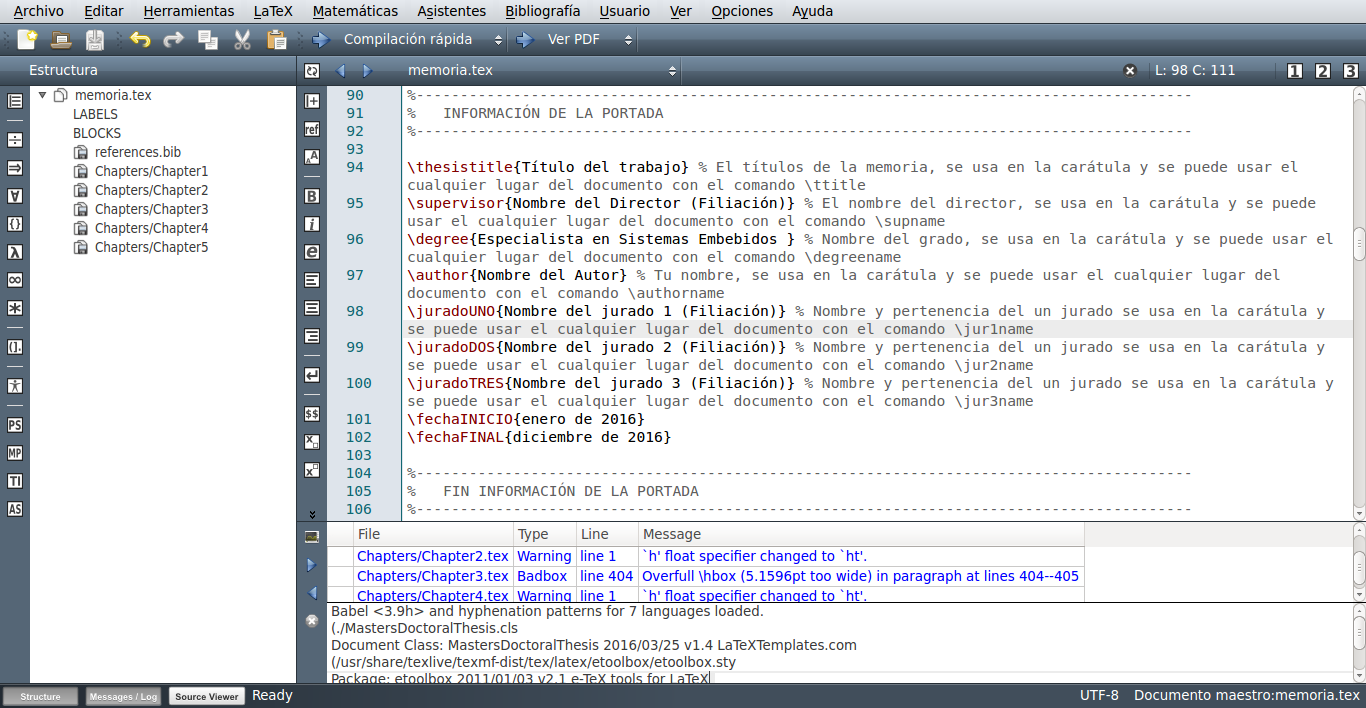
\includegraphics[width=.5\textwidth]{./Figures/texmaker.png}
	\caption{Entorno de trabajo de texMaker.}
	\label{fig:texmaker}
\end{figure}

\vspace{1cm}

Notar que existe una vista llamada Estructura a la izquierda de la interfaz que nos permite abrir desde dentro del programa los archivos individuales de los capítulos.  A la derecha se encuentra una vista con el archivo propiamente dicho para su edición. Hacia la parte inferior se encuentra una vista del log con información de los resultados de la compilación.  En esta última vista pueden aparecen advertencias o \textit{warning}, que normalmente pueden ser ignorados, y los errores que se indican en color rojo y deben resolverse para que se genere el PDF de salida.

Recordar que el archivo que se debe compilar con PDFLaTeX es \file{memoria.tex}, si se tratara de compilar alguno de los capítulos saldría un error.  Para salvar la molestia de tener que cambiar de archivo para compilar cada vez que se realice una modificación en un capítulo, se puede definir el archivo \file{memoria.tex} como ``documento maestro'' yendo al menú opciones -> ``definir documento actual como documento maestro'', lo que permite compilar con PDFLaTeX memoria.tex directamente desde cualquier archivo que se esté modificando . Se muestra esta opción en la figura \ref{fig:docMaestro}.

\begin{figure}[h]
	\centering
	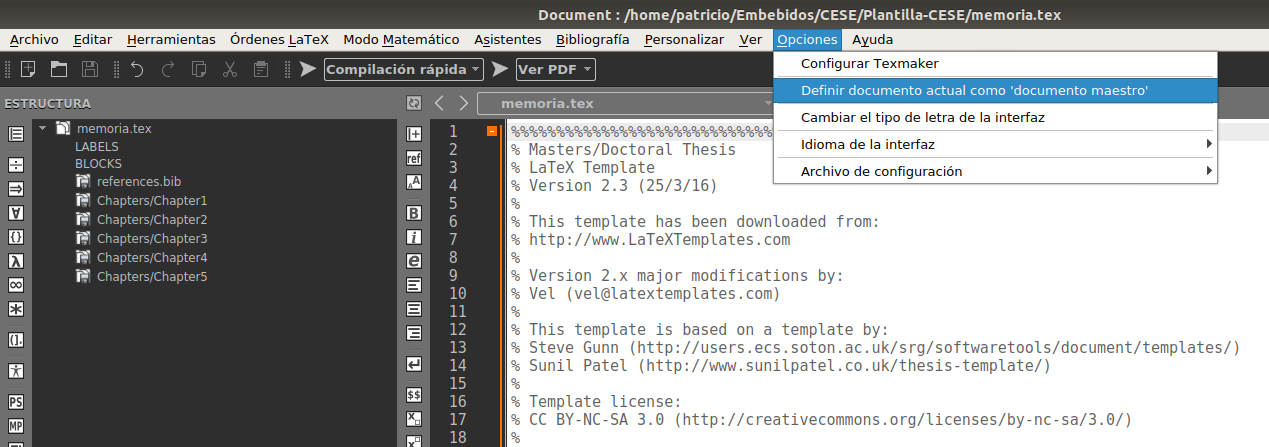
\includegraphics[width=\textwidth]{./Figures/docMaestro.png}
	\caption{Definir memoria.tex como documento maestro.}
	\label{fig:docMaestro}
\end{figure}

En el menú herramientas se encuentran las opciones de compilación.  Para producir un archivo PDF a partir de un archivo .tex se debe ejecutar PDFLaTeX (el shortcut es F6). Para incorporar nueva bibliografía se debe utilizar la opción BibTeX del mismo menú herramientas (el shortcut es F11).

Notar que para actualizar las tablas de contenidos se debe ejecutar PDFLaTeX dos veces.  Esto se debe a que es necesario actualizar algunos archivos auxiliares antes de obtener el resultado final.  En forma similar, para actualizar las referencias se debe ejecutar primero PDFLaTeX, después BibTeX y finalmente PDFLaTeX dos veces por idénticos motivos.

\section{Personalizando la plantilla, el archivo \file{memoria.tex}}
\label{sec:FillingFile}

Para personalizar la plantilla se debe incorporar la información propia en los distintos archivos \file{.tex}. 

Primero abrir \file{memoria.tex} con TexMaker (o el editor de su preferencia). Se debe ubicar dentro del archivo el bloque de código titulado \emph{INFORMACIÓN DE LA PORTADA} donde se deben incorporar los primeros datos personales con los que se construirá automáticamente la portada.


%----------------------------------------------------------------------------------------

\section{El código del archivo \file{memoria.tex} explicado}

El archivo \file{memoria.tex} contiene la estructura del documento y es el archivo de mayor jerarquía de la memoria.  Podría ser equiparable a la función \emph{main()} de un programa en C, o mejor dicho al archivo fuente .c donde se encuentra definida la función main().

La estructura básica de cualquier documento de \LaTeX{} comienza con la definición de clase del documento, es seguida por un preámbulo donde se pueden agregar funcionalidades con el uso de \texttt{paquetes} (equiparables a bibliotecas de C), y finalmente, termina con el cuerpo del documento, donde irá el contenido de la memoria.

\lstset{%
  basicstyle=\small\ttfamily,
  language=[LaTeX]{TeX}
}

\begin{lstlisting}
\documentclass{article}  <- Definicion de clase
\usepackage{listings}	 <- Preambulo

\begin{document}	 <- Comienzo del contenido propio 
	Hello world!
\end{document}
\end{lstlisting}


El archivo \file{memoria.tex} se encuentra densamente comentado para explicar qué páginas, secciones y elementos de formato está creando el código \LaTeX{} en cada línea. El código está dividido en bloques con nombres en mayúsculas para que resulte evidente qué es lo que hace esa porción de código en particular. Inicialmente puede parecer que hay mucho código \LaTeX{}, pero es principalmente código para dar formato a la memoria por lo que no requiere intervención del usuario de la plantilla.  Sí se deben personalizar con su información los bloques indicados como:

\begin{itemize}
	\item Informacion de la memoria
	\item Resumen
	\item Agradecimientos
	\item Dedicatoria
\end{itemize}

El índice de contenidos, las listas de figura de tablas se generan en forma automática y no requieren intervención ni edición manual por parte del usuario de la plantilla. 

En la parte final del documento se encuentran los capítulos y los apéndices.  Por defecto se incluyen los 5 capítulos propuestos que se encuentran en la carpeta /Chapters. Cada capítulo se debe escribir en un archivo .tex separado y se debe poner en la carpeta \emph{Chapters} con el nombre \file{Chapter1}, \file{Chapter2}, etc\ldots El código para incluir capítulos desde archivos externos se muestra a continuación.

\begin{verbatim}
	% Chapter 1

\chapter{Introducción general} % Main chapter title

\label{Chapter1} % For referencing the chapter elsewhere, use \ref{Chapter1} 
\label{IntroGeneral}

%----------------------------------------------------------------------------------------

% Define some commands to keep the formatting separated from the content 
\newcommand{\keyword}[1]{\textbf{#1}}
\newcommand{\tabhead}[1]{\textbf{#1}}
\newcommand{\code}[1]{\texttt{#1}}
\newcommand{\file}[1]{\texttt{\bfseries#1}}
\newcommand{\option}[1]{\texttt{\itshape#1}}
\newcommand{\grados}{$^{\circ}$}

%----------------------------------------------------------------------------------------

%\section{Introducción}

%----------------------------------------------------------------------------------------
\section{Aprendiendo \LaTeX{}}

\LaTeX{} no es \textsc{WYSIWYG} (What You See is What You Get), a diferencia de los procesadores de texto como Microsoft Word o Pages de Apple o incluso LibreOffice en el mundo open-source. En lugar de ello, un documento escrito para \LaTeX{} es en realidad un archivo de texto simple o llano que \emph{no contiene formato} . Nosotros le decimos a \LaTeX{} cómo deseamos que se aplique el formato en el documento final escribiendo comandos simples entre el texto, por ejemplo, si quiero usar texto en itálicas para dar énfasis, escribo \verb|\it{texto}| y pongo el texto que quiero en itálicas entre medio de las llaves. Esto significa que \LaTeX{} es un lenguaje del tipo \enquote{mark-up}, muy parecido a HTML.

\subsection{Una introducción (no tan corta) a \LaTeX{}}

Si sos nuevo en \LaTeX{}, hay un muy buen libro electrónico - disponible gratuitamente en Internet como un archivo PDF - llamado, \enquote{A (not so short) Introduction to \LaTeX{}}. El título del libro es generalmente acortado a simplemente \emph{lshort}. Puede descargar la versión más reciente en inglés (ya que se actualiza de vez en cuando) desde aquí:
\url{http://www.ctan.org/tex-archive/info/lshort/english/lshort.pdf}

Se puede encontrar la versión en español en la lista en esta página: \url{http://www.ctan.org/tex-archive/info/lshort/}

\subsubsection{Una subsubsección}

Acá tiene un ejemplo de una ``subsubsección'' que es el cuarto nivel de ordenamiento del texto, después de capítulo, sección y subsección.  Como se puede ver, las subsubsecciones no van numeradas en el cuerpo del documento ni en el índice.  El formato está definido por la plantilla y no debe ser modificado.

\subsection{Guía matemática rápida para \LaTeX{}}

Si estás escribiendo un documento con mucho contenido matemático, entonces es posible que desees leer el documento de la AMS (American Mathematical Society) llamado, \enquote{A Short Math Guide for \LaTeX{}}. Se puede encontrar en línea en el siguiente link: \url{http://www.ams.org/tex/amslatex.html} en la sección \enquote{Additional Documentation} hacia la parte inferior de la página.


%----------------------------------------------------------------------------------------

\section{Utilizando esta plantilla}

Si estás familiarizado con \LaTeX{}, entonces podés explorar la estructura de directorios de esta plantilla y proceder a personalizarla agregando tu información en el bloque \emph{INFORMACIÓN DE LA PORTADA} en el archivo \file{memoria.tex}.  

Se puede continuar luego modificando el resto de los archivos siguiendo los lineamientos que se describen en la sección \ref{sec:FillingFile} en la página \pageref{sec:FillingFile}.

Debés asegurarte de leer el capítulo \ref{Chapter2} acerca de las convenciones utilizadas para las Memoria de los Trabajos Finales de la \degreename.

Si sos nuevo en \LaTeX{}, se recomienda que continúes leyendo el documento ya que contiene información básica para aprovechar el potencial de esta herramienta.


%----------------------------------------------------------------------------------------

\section{Qué incluye esta plantilla}

\subsection{Carpetas}

Esta plantilla se distribuye como una único archivo .zip que se puede descomprimir en varios archivos y carpetas. Asimismo, se puede consultar el repositorio git para obtener la última versión de los archivos, \url{https://github.com/patriciobos/Plantilla-CESE.git}. Los nombres de las carpetas son, o pretender ser, auto-explicativos.

\keyword{Appendices} -- Esta es la carpeta donde se deben poner los apéndices. Cada apéndice debe ir en su propio archivo \file{.tex}. Se incluye un ejemplo y una plantilla en la carpeta.

\keyword{Chapters} -- Esta es la carpeta donde se deben poner los capítulos de la memoria. Cada capítulo debe ir un su propio archivo \file{.tex} por separado.  Se ofrece por defecto, la siguiente estructura de capítulos y se recomienda su utilización dentro de lo posible:

\begin{itemize}
\item Capítulo 1: Introducción general	
\item Capítulo 2: Introducción específica
\item Capítulo 3: Diseño e implementación
\item Capítulo 4: Ensayos y resultados
\item Capítulo 5: Conclusiones

\end{itemize}

Esta estructura de capítulos es la que se recomienda para las memorias de la especialización.

\keyword{Figures} -- Esta carpeta contiene todas las figuras de la memoria.  Estas son las versiones finales de las imágenes que van a ser incluidas en la memoria.  Pueden ser imágenes en formato \textit{raster}\footnote{\url{https://en.wikipedia.org/wiki/Raster_graphics}} como \file{.png}, \file{.jpg} o en formato vectoriales\footnote{\url{https://en.wikipedia.org/wiki/Vector_graphics}} como \file{.pdf}, \file{.ps}.  Se debe notar que utilizar imágenes vectoriales disminuye notablemente el peso del documento final y acelera el tiempo de compilación por lo que es recomendable su utilización siempre que sea posible.

\subsection{Archivos}

También están incluidos varios archivos, la mayoría de ellos son de texto plano y se puede ver su contenido en un editor de texto. Después de la compilación inicial, se verá que más archivos auxiliares son creados por \ LaTeX{} o BibTeX, pero son de uso interno y no es necesario hacer nada en particular con ellos.  Toda la información necesaria para compilar el documento se encuentra en los archivos \file{.tex}, \file{.bib}, \file{.cls} y en las imágenes de la carpeta Figures.

\keyword{referencias.bib} - este es un archivo importante que contiene toda la información de referencias bibliográficas que se utilizarán para las citas en la memoria en conjunto con BibTeX. Usted puede escribir las entradas bibliográficas en forma manual, aunque existen también programas de gestión de referencias que facilitan la creación y gestión de las referencias y permiten exportarlas en formato BibTeX.  También hay disponibles sitios web como \url{books.google.com} que permiten obtener toda la información necesaria para una cita en formato BibTeX. Ver sección \ref{sec:biblio}

\keyword{MastersDoctoralThesis.cls} -- este es un archivo importante. Es el archivos con la clase que le informa a \LaTeX{} cómo debe dar formato a la memoria. El usuario de la plantilla no debería necesitar modificar nada de este archivo.

\keyword{memoria.pdf} -- esta es su memoria con una tipografía bellamente compuesta (en formato de archivo PDF) creado por \LaTeX{}. Se distribuye con la plantilla y después de compilar por primera vez sin hacer ningún cambio se debería obtener una versión idéntica a este documento.

\keyword{memoria.tex} -- este es un archivo importante. Este es el archivo que tiene que compilar \LaTeX{} para producir la memoria como un archivo PDF. Contiene un marco de trabajo y estructuras que le indican a \LaTeX{} cómo diagramar la memoria.  Está altamente comentado para que se pueda entender qué es lo que realiza cada línea de código y por qué está incluida en ese lugar.  En este archivo se debe completar la información personalizada de las primeras sección según se indica en la sección \ref{sec:FillingFile}.

Archivos que \emph{no} forman parte de la distribución de la plantilla pero que son generados por \LaTeX{} como archivos auxiliares necesarios para la producción de la memoria.pdf son:

\keyword{memoria.aux} -- este es un archivo auxiliar generado por \LaTeX{}, si se borra \LaTeX{} simplemente lo regenera cuando se compila el archivo principal \file{memoria.tex}.

\keyword{memoria.bbl} -- este es un archivo auxiliar generado por BibTeX, si se borra BibTeX simplemente lo regenera cuando se compila el archivo principal \file{memoria.tex}. Mientras que el archivo \file{.bib} contiene todas las referencias que hay, este archivo \file{.bbl} contine sólo las referencias que han sido citadas y se utiliza para la construcción de la bibiografía.

\keyword{memoria.blg} -- este es un archivo auxiliar generado por BibTeX, si se borra BibTeX simplemente lo regenera cuando se compila el archivo principal \file{memoria.tex}.

\keyword{memoria.lof} -- este es un archivo auxiliar generado por \LaTeX{}, si se borra \LaTeX{} simplemente lo regenera cuando se compila el archivo principal \file{memoria.tex}.  Le indica a \LaTeX{} cómo construir la sección \emph{Lista de Figuras}.
 
\keyword{memoria.log} --  este es un archivo auxiliar generado por \LaTeX{}, si se borra \LaTeX{} simplemente lo regenera cuando se compila el archivo principal \file{memoria.tex}. Contiene mensajes de \LaTeX{}. Si se reciben errores o advertencias durante la compilación, se guardan en este archivo \file{.log}.

\keyword{memoria.lot} -- este es un archivo auxiliar generado por \LaTeX{}, si se borra \LaTeX{} simplemente lo regenera cuando se compila el archivo principal \file{memoria.tex}.  Le indica a \LaTeX{} cómo construir la sección \emph{Lista de Tablas}.

\keyword{memoria.out} -- este es un archivo auxiliar generado por \LaTeX{}, si se borra \LaTeX{} simplemente lo regenera cuando se compila el archivo principal \file{memoria.tex}.

De esta larga lista de archivos, sólo aquellos con la extensión \file{.bib}, \file{.cls} y \file{.tex} son importantes.  Los otros archivos auxiliares pueden ser ignorados o borrados ya que \LaTeX{} y BibTeX los regenerarán durante la compilación.

%----------------------------------------------------------------------------------------

\section{Entorno de trabajo}

Ante de comenzar a editar la plantilla debemos tener un editor \LaTeX{} instalado en nuestra computadora.  En forma análoga a lo que sucede en lenguaje C, que se puede crear y editar código con casi cualquier editor, existen ciertos entornos de trabajo que nos pueden simplificar mucho la tarea.  En este sentido, se recomienda, sobre todo para los principiantes en \LaTeX{} la utilización de TexMaker, un programa gratuito y multi-plantaforma que está disponible tanto para windows como para sistemas GNU/linux.

La versión más reciente de TexMaker es la 4.5 y se puede descargar del siguiente link: \url{http://www.xm1math.net/texmaker/download.html}. Se puede consultar el manual de usuario en el siguiente link: \url{http://www.xm1math.net/texmaker/doc.html}.
 

\subsection{Paquetes adicionales}

Si bien durante el proceso de instalación de TexMaker, o cualquier otro editor que se haya elegido, se instalarán en el sistema los paquetes básicos necesarios para trabajar con \LaTeX{}, la plantilla de los trabajos de Especialización y Maestría requieren de paquete adicionales.

Se indican a continuación los comandos que se deben introducir en la consola de Ubuntu (ctrl + alt + t) para instalarlos:

\begin{lstlisting}[language=bash]
  $ sudo apt install texlive-lang-spanish texlive-science 
  $ sudo apt install texlive-bibtex-extra biber
  $ sudo apt install texlive texlive-fonts-recommended
  $ sudo apt install texlive-latex-extra
\end{lstlisting}


\subsection{Configurando TexMaker}



Una vez instalado el programa y los paquetes adicionales se debe abrir el archivo memoria.tex con el editor para ver una pantalla similar a la que se puede apreciar en la figura \ref{fig:texmaker}. 
Una vez instalado el programa y los paquetes adicionales se debe abrir el archivo memoria.tex con el editor para ver una pantalla similar a la que se puede apreciar en la figura \ref{fig:texmaker}. 
Una vez instalado el programa y los paquetes adicionales se debe abrir el archivo memoria.tex con el editor para ver una pantalla similar a la que se puede apreciar en la figura \ref{fig:texmaker}. 
Una vez instalado el programa y los paquetes adicionales se debe abrir el archivo memoria.tex con el editor para ver una pantalla similar a la que se puede apreciar en la figura \ref{fig:texmaker}. 

\vspace{1cm}

\begin{figure}[htbp]
	\centering
	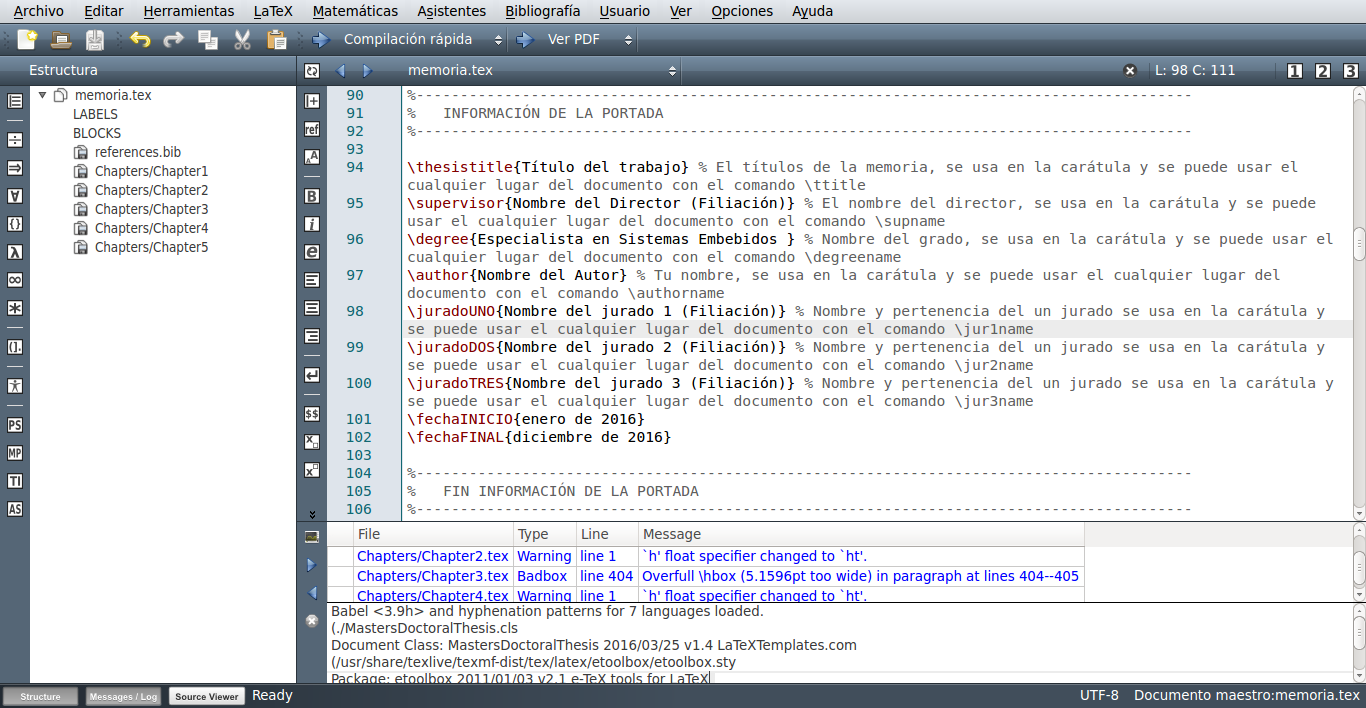
\includegraphics[width=.5\textwidth]{./Figures/texmaker.png}
	\caption{Entorno de trabajo de texMaker.}
	\label{fig:texmaker}
\end{figure}

\vspace{1cm}

Notar que existe una vista llamada Estructura a la izquierda de la interfaz que nos permite abrir desde dentro del programa los archivos individuales de los capítulos.  A la derecha se encuentra una vista con el archivo propiamente dicho para su edición. Hacia la parte inferior se encuentra una vista del log con información de los resultados de la compilación.  En esta última vista pueden aparecen advertencias o \textit{warning}, que normalmente pueden ser ignorados, y los errores que se indican en color rojo y deben resolverse para que se genere el PDF de salida.

Recordar que el archivo que se debe compilar con PDFLaTeX es \file{memoria.tex}, si se tratara de compilar alguno de los capítulos saldría un error.  Para salvar la molestia de tener que cambiar de archivo para compilar cada vez que se realice una modificación en un capítulo, se puede definir el archivo \file{memoria.tex} como ``documento maestro'' yendo al menú opciones -> ``definir documento actual como documento maestro'', lo que permite compilar con PDFLaTeX memoria.tex directamente desde cualquier archivo que se esté modificando . Se muestra esta opción en la figura \ref{fig:docMaestro}.

\begin{figure}[h]
	\centering
	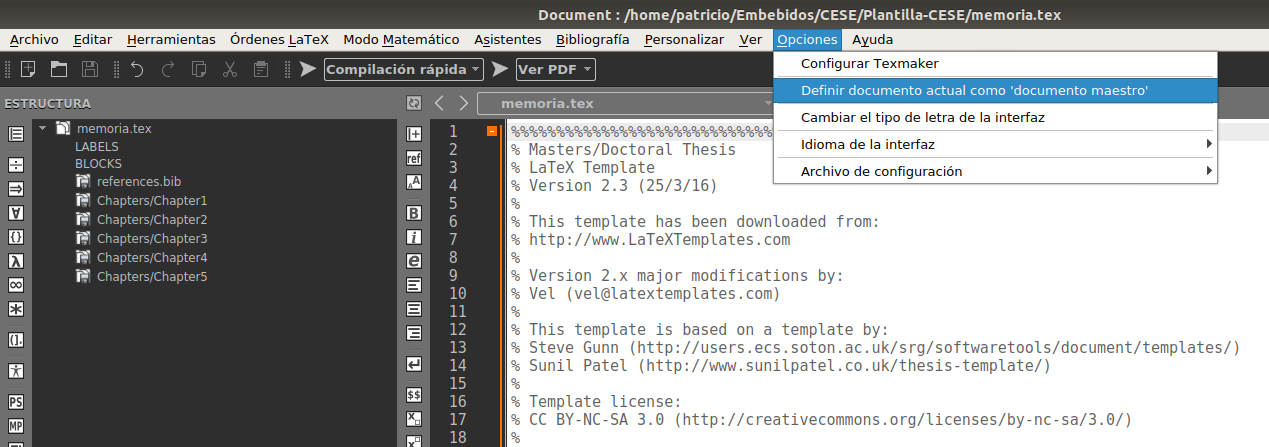
\includegraphics[width=\textwidth]{./Figures/docMaestro.png}
	\caption{Definir memoria.tex como documento maestro.}
	\label{fig:docMaestro}
\end{figure}

En el menú herramientas se encuentran las opciones de compilación.  Para producir un archivo PDF a partir de un archivo .tex se debe ejecutar PDFLaTeX (el shortcut es F6). Para incorporar nueva bibliografía se debe utilizar la opción BibTeX del mismo menú herramientas (el shortcut es F11).

Notar que para actualizar las tablas de contenidos se debe ejecutar PDFLaTeX dos veces.  Esto se debe a que es necesario actualizar algunos archivos auxiliares antes de obtener el resultado final.  En forma similar, para actualizar las referencias se debe ejecutar primero PDFLaTeX, después BibTeX y finalmente PDFLaTeX dos veces por idénticos motivos.

\section{Personalizando la plantilla, el archivo \file{memoria.tex}}
\label{sec:FillingFile}

Para personalizar la plantilla se debe incorporar la información propia en los distintos archivos \file{.tex}. 

Primero abrir \file{memoria.tex} con TexMaker (o el editor de su preferencia). Se debe ubicar dentro del archivo el bloque de código titulado \emph{INFORMACIÓN DE LA PORTADA} donde se deben incorporar los primeros datos personales con los que se construirá automáticamente la portada.


%----------------------------------------------------------------------------------------

\section{El código del archivo \file{memoria.tex} explicado}

El archivo \file{memoria.tex} contiene la estructura del documento y es el archivo de mayor jerarquía de la memoria.  Podría ser equiparable a la función \emph{main()} de un programa en C, o mejor dicho al archivo fuente .c donde se encuentra definida la función main().

La estructura básica de cualquier documento de \LaTeX{} comienza con la definición de clase del documento, es seguida por un preámbulo donde se pueden agregar funcionalidades con el uso de \texttt{paquetes} (equiparables a bibliotecas de C), y finalmente, termina con el cuerpo del documento, donde irá el contenido de la memoria.

\lstset{%
  basicstyle=\small\ttfamily,
  language=[LaTeX]{TeX}
}

\begin{lstlisting}
\documentclass{article}  <- Definicion de clase
\usepackage{listings}	 <- Preambulo

\begin{document}	 <- Comienzo del contenido propio 
	Hello world!
\end{document}
\end{lstlisting}


El archivo \file{memoria.tex} se encuentra densamente comentado para explicar qué páginas, secciones y elementos de formato está creando el código \LaTeX{} en cada línea. El código está dividido en bloques con nombres en mayúsculas para que resulte evidente qué es lo que hace esa porción de código en particular. Inicialmente puede parecer que hay mucho código \LaTeX{}, pero es principalmente código para dar formato a la memoria por lo que no requiere intervención del usuario de la plantilla.  Sí se deben personalizar con su información los bloques indicados como:

\begin{itemize}
	\item Informacion de la memoria
	\item Resumen
	\item Agradecimientos
	\item Dedicatoria
\end{itemize}

El índice de contenidos, las listas de figura de tablas se generan en forma automática y no requieren intervención ni edición manual por parte del usuario de la plantilla. 

En la parte final del documento se encuentran los capítulos y los apéndices.  Por defecto se incluyen los 5 capítulos propuestos que se encuentran en la carpeta /Chapters. Cada capítulo se debe escribir en un archivo .tex separado y se debe poner en la carpeta \emph{Chapters} con el nombre \file{Chapter1}, \file{Chapter2}, etc\ldots El código para incluir capítulos desde archivos externos se muestra a continuación.

\begin{verbatim}
	% Chapter 1

\chapter{Introducción general} % Main chapter title

\label{Chapter1} % For referencing the chapter elsewhere, use \ref{Chapter1} 
\label{IntroGeneral}

%----------------------------------------------------------------------------------------

% Define some commands to keep the formatting separated from the content 
\newcommand{\keyword}[1]{\textbf{#1}}
\newcommand{\tabhead}[1]{\textbf{#1}}
\newcommand{\code}[1]{\texttt{#1}}
\newcommand{\file}[1]{\texttt{\bfseries#1}}
\newcommand{\option}[1]{\texttt{\itshape#1}}
\newcommand{\grados}{$^{\circ}$}

%----------------------------------------------------------------------------------------

%\section{Introducción}

%----------------------------------------------------------------------------------------
\section{Aprendiendo \LaTeX{}}

\LaTeX{} no es \textsc{WYSIWYG} (What You See is What You Get), a diferencia de los procesadores de texto como Microsoft Word o Pages de Apple o incluso LibreOffice en el mundo open-source. En lugar de ello, un documento escrito para \LaTeX{} es en realidad un archivo de texto simple o llano que \emph{no contiene formato} . Nosotros le decimos a \LaTeX{} cómo deseamos que se aplique el formato en el documento final escribiendo comandos simples entre el texto, por ejemplo, si quiero usar texto en itálicas para dar énfasis, escribo \verb|\it{texto}| y pongo el texto que quiero en itálicas entre medio de las llaves. Esto significa que \LaTeX{} es un lenguaje del tipo \enquote{mark-up}, muy parecido a HTML.

\subsection{Una introducción (no tan corta) a \LaTeX{}}

Si sos nuevo en \LaTeX{}, hay un muy buen libro electrónico - disponible gratuitamente en Internet como un archivo PDF - llamado, \enquote{A (not so short) Introduction to \LaTeX{}}. El título del libro es generalmente acortado a simplemente \emph{lshort}. Puede descargar la versión más reciente en inglés (ya que se actualiza de vez en cuando) desde aquí:
\url{http://www.ctan.org/tex-archive/info/lshort/english/lshort.pdf}

Se puede encontrar la versión en español en la lista en esta página: \url{http://www.ctan.org/tex-archive/info/lshort/}

\subsubsection{Una subsubsección}

Acá tiene un ejemplo de una ``subsubsección'' que es el cuarto nivel de ordenamiento del texto, después de capítulo, sección y subsección.  Como se puede ver, las subsubsecciones no van numeradas en el cuerpo del documento ni en el índice.  El formato está definido por la plantilla y no debe ser modificado.

\subsection{Guía matemática rápida para \LaTeX{}}

Si estás escribiendo un documento con mucho contenido matemático, entonces es posible que desees leer el documento de la AMS (American Mathematical Society) llamado, \enquote{A Short Math Guide for \LaTeX{}}. Se puede encontrar en línea en el siguiente link: \url{http://www.ams.org/tex/amslatex.html} en la sección \enquote{Additional Documentation} hacia la parte inferior de la página.


%----------------------------------------------------------------------------------------

\section{Utilizando esta plantilla}

Si estás familiarizado con \LaTeX{}, entonces podés explorar la estructura de directorios de esta plantilla y proceder a personalizarla agregando tu información en el bloque \emph{INFORMACIÓN DE LA PORTADA} en el archivo \file{memoria.tex}.  

Se puede continuar luego modificando el resto de los archivos siguiendo los lineamientos que se describen en la sección \ref{sec:FillingFile} en la página \pageref{sec:FillingFile}.

Debés asegurarte de leer el capítulo \ref{Chapter2} acerca de las convenciones utilizadas para las Memoria de los Trabajos Finales de la \degreename.

Si sos nuevo en \LaTeX{}, se recomienda que continúes leyendo el documento ya que contiene información básica para aprovechar el potencial de esta herramienta.


%----------------------------------------------------------------------------------------

\section{Qué incluye esta plantilla}

\subsection{Carpetas}

Esta plantilla se distribuye como una único archivo .zip que se puede descomprimir en varios archivos y carpetas. Asimismo, se puede consultar el repositorio git para obtener la última versión de los archivos, \url{https://github.com/patriciobos/Plantilla-CESE.git}. Los nombres de las carpetas son, o pretender ser, auto-explicativos.

\keyword{Appendices} -- Esta es la carpeta donde se deben poner los apéndices. Cada apéndice debe ir en su propio archivo \file{.tex}. Se incluye un ejemplo y una plantilla en la carpeta.

\keyword{Chapters} -- Esta es la carpeta donde se deben poner los capítulos de la memoria. Cada capítulo debe ir un su propio archivo \file{.tex} por separado.  Se ofrece por defecto, la siguiente estructura de capítulos y se recomienda su utilización dentro de lo posible:

\begin{itemize}
\item Capítulo 1: Introducción general	
\item Capítulo 2: Introducción específica
\item Capítulo 3: Diseño e implementación
\item Capítulo 4: Ensayos y resultados
\item Capítulo 5: Conclusiones

\end{itemize}

Esta estructura de capítulos es la que se recomienda para las memorias de la especialización.

\keyword{Figures} -- Esta carpeta contiene todas las figuras de la memoria.  Estas son las versiones finales de las imágenes que van a ser incluidas en la memoria.  Pueden ser imágenes en formato \textit{raster}\footnote{\url{https://en.wikipedia.org/wiki/Raster_graphics}} como \file{.png}, \file{.jpg} o en formato vectoriales\footnote{\url{https://en.wikipedia.org/wiki/Vector_graphics}} como \file{.pdf}, \file{.ps}.  Se debe notar que utilizar imágenes vectoriales disminuye notablemente el peso del documento final y acelera el tiempo de compilación por lo que es recomendable su utilización siempre que sea posible.

\subsection{Archivos}

También están incluidos varios archivos, la mayoría de ellos son de texto plano y se puede ver su contenido en un editor de texto. Después de la compilación inicial, se verá que más archivos auxiliares son creados por \ LaTeX{} o BibTeX, pero son de uso interno y no es necesario hacer nada en particular con ellos.  Toda la información necesaria para compilar el documento se encuentra en los archivos \file{.tex}, \file{.bib}, \file{.cls} y en las imágenes de la carpeta Figures.

\keyword{referencias.bib} - este es un archivo importante que contiene toda la información de referencias bibliográficas que se utilizarán para las citas en la memoria en conjunto con BibTeX. Usted puede escribir las entradas bibliográficas en forma manual, aunque existen también programas de gestión de referencias que facilitan la creación y gestión de las referencias y permiten exportarlas en formato BibTeX.  También hay disponibles sitios web como \url{books.google.com} que permiten obtener toda la información necesaria para una cita en formato BibTeX. Ver sección \ref{sec:biblio}

\keyword{MastersDoctoralThesis.cls} -- este es un archivo importante. Es el archivos con la clase que le informa a \LaTeX{} cómo debe dar formato a la memoria. El usuario de la plantilla no debería necesitar modificar nada de este archivo.

\keyword{memoria.pdf} -- esta es su memoria con una tipografía bellamente compuesta (en formato de archivo PDF) creado por \LaTeX{}. Se distribuye con la plantilla y después de compilar por primera vez sin hacer ningún cambio se debería obtener una versión idéntica a este documento.

\keyword{memoria.tex} -- este es un archivo importante. Este es el archivo que tiene que compilar \LaTeX{} para producir la memoria como un archivo PDF. Contiene un marco de trabajo y estructuras que le indican a \LaTeX{} cómo diagramar la memoria.  Está altamente comentado para que se pueda entender qué es lo que realiza cada línea de código y por qué está incluida en ese lugar.  En este archivo se debe completar la información personalizada de las primeras sección según se indica en la sección \ref{sec:FillingFile}.

Archivos que \emph{no} forman parte de la distribución de la plantilla pero que son generados por \LaTeX{} como archivos auxiliares necesarios para la producción de la memoria.pdf son:

\keyword{memoria.aux} -- este es un archivo auxiliar generado por \LaTeX{}, si se borra \LaTeX{} simplemente lo regenera cuando se compila el archivo principal \file{memoria.tex}.

\keyword{memoria.bbl} -- este es un archivo auxiliar generado por BibTeX, si se borra BibTeX simplemente lo regenera cuando se compila el archivo principal \file{memoria.tex}. Mientras que el archivo \file{.bib} contiene todas las referencias que hay, este archivo \file{.bbl} contine sólo las referencias que han sido citadas y se utiliza para la construcción de la bibiografía.

\keyword{memoria.blg} -- este es un archivo auxiliar generado por BibTeX, si se borra BibTeX simplemente lo regenera cuando se compila el archivo principal \file{memoria.tex}.

\keyword{memoria.lof} -- este es un archivo auxiliar generado por \LaTeX{}, si se borra \LaTeX{} simplemente lo regenera cuando se compila el archivo principal \file{memoria.tex}.  Le indica a \LaTeX{} cómo construir la sección \emph{Lista de Figuras}.
 
\keyword{memoria.log} --  este es un archivo auxiliar generado por \LaTeX{}, si se borra \LaTeX{} simplemente lo regenera cuando se compila el archivo principal \file{memoria.tex}. Contiene mensajes de \LaTeX{}. Si se reciben errores o advertencias durante la compilación, se guardan en este archivo \file{.log}.

\keyword{memoria.lot} -- este es un archivo auxiliar generado por \LaTeX{}, si se borra \LaTeX{} simplemente lo regenera cuando se compila el archivo principal \file{memoria.tex}.  Le indica a \LaTeX{} cómo construir la sección \emph{Lista de Tablas}.

\keyword{memoria.out} -- este es un archivo auxiliar generado por \LaTeX{}, si se borra \LaTeX{} simplemente lo regenera cuando se compila el archivo principal \file{memoria.tex}.

De esta larga lista de archivos, sólo aquellos con la extensión \file{.bib}, \file{.cls} y \file{.tex} son importantes.  Los otros archivos auxiliares pueden ser ignorados o borrados ya que \LaTeX{} y BibTeX los regenerarán durante la compilación.

%----------------------------------------------------------------------------------------

\section{Entorno de trabajo}

Ante de comenzar a editar la plantilla debemos tener un editor \LaTeX{} instalado en nuestra computadora.  En forma análoga a lo que sucede en lenguaje C, que se puede crear y editar código con casi cualquier editor, existen ciertos entornos de trabajo que nos pueden simplificar mucho la tarea.  En este sentido, se recomienda, sobre todo para los principiantes en \LaTeX{} la utilización de TexMaker, un programa gratuito y multi-plantaforma que está disponible tanto para windows como para sistemas GNU/linux.

La versión más reciente de TexMaker es la 4.5 y se puede descargar del siguiente link: \url{http://www.xm1math.net/texmaker/download.html}. Se puede consultar el manual de usuario en el siguiente link: \url{http://www.xm1math.net/texmaker/doc.html}.
 

\subsection{Paquetes adicionales}

Si bien durante el proceso de instalación de TexMaker, o cualquier otro editor que se haya elegido, se instalarán en el sistema los paquetes básicos necesarios para trabajar con \LaTeX{}, la plantilla de los trabajos de Especialización y Maestría requieren de paquete adicionales.

Se indican a continuación los comandos que se deben introducir en la consola de Ubuntu (ctrl + alt + t) para instalarlos:

\begin{lstlisting}[language=bash]
  $ sudo apt install texlive-lang-spanish texlive-science 
  $ sudo apt install texlive-bibtex-extra biber
  $ sudo apt install texlive texlive-fonts-recommended
  $ sudo apt install texlive-latex-extra
\end{lstlisting}


\subsection{Configurando TexMaker}



Una vez instalado el programa y los paquetes adicionales se debe abrir el archivo memoria.tex con el editor para ver una pantalla similar a la que se puede apreciar en la figura \ref{fig:texmaker}. 
Una vez instalado el programa y los paquetes adicionales se debe abrir el archivo memoria.tex con el editor para ver una pantalla similar a la que se puede apreciar en la figura \ref{fig:texmaker}. 
Una vez instalado el programa y los paquetes adicionales se debe abrir el archivo memoria.tex con el editor para ver una pantalla similar a la que se puede apreciar en la figura \ref{fig:texmaker}. 
Una vez instalado el programa y los paquetes adicionales se debe abrir el archivo memoria.tex con el editor para ver una pantalla similar a la que se puede apreciar en la figura \ref{fig:texmaker}. 

\vspace{1cm}

\begin{figure}[htbp]
	\centering
	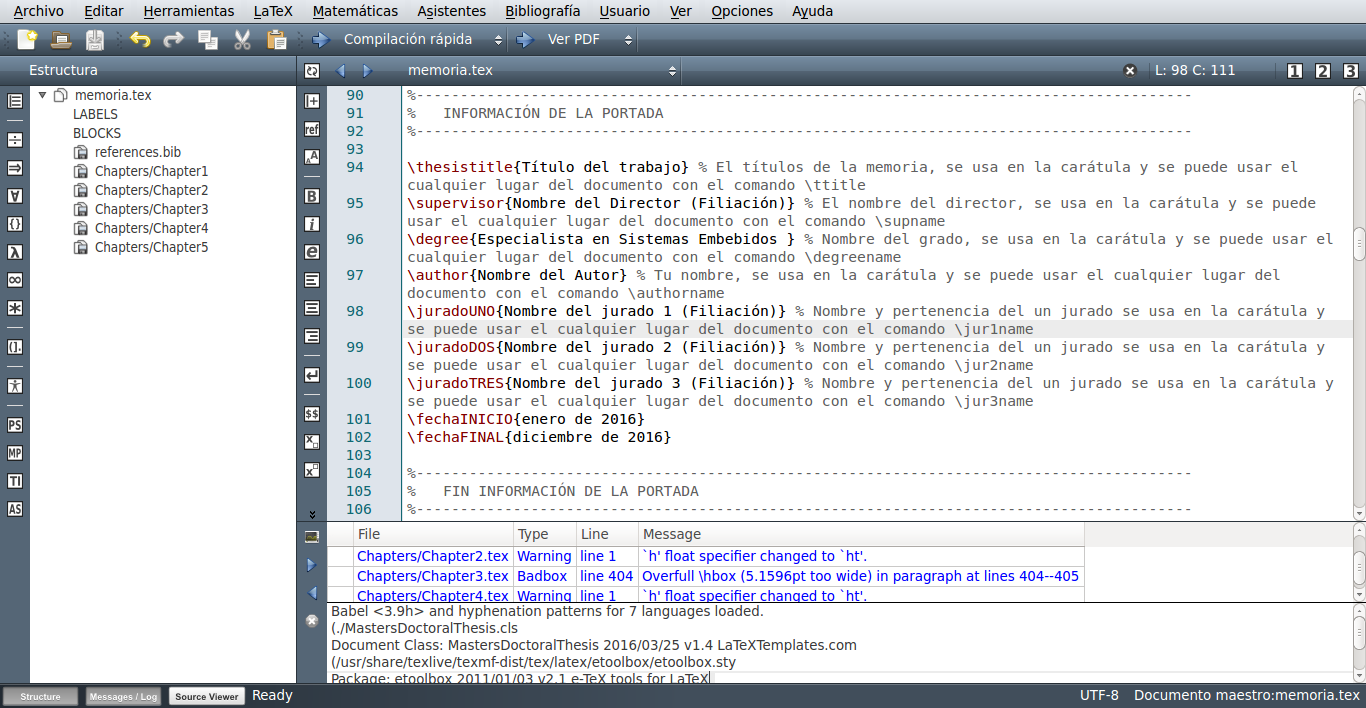
\includegraphics[width=.5\textwidth]{./Figures/texmaker.png}
	\caption{Entorno de trabajo de texMaker.}
	\label{fig:texmaker}
\end{figure}

\vspace{1cm}

Notar que existe una vista llamada Estructura a la izquierda de la interfaz que nos permite abrir desde dentro del programa los archivos individuales de los capítulos.  A la derecha se encuentra una vista con el archivo propiamente dicho para su edición. Hacia la parte inferior se encuentra una vista del log con información de los resultados de la compilación.  En esta última vista pueden aparecen advertencias o \textit{warning}, que normalmente pueden ser ignorados, y los errores que se indican en color rojo y deben resolverse para que se genere el PDF de salida.

Recordar que el archivo que se debe compilar con PDFLaTeX es \file{memoria.tex}, si se tratara de compilar alguno de los capítulos saldría un error.  Para salvar la molestia de tener que cambiar de archivo para compilar cada vez que se realice una modificación en un capítulo, se puede definir el archivo \file{memoria.tex} como ``documento maestro'' yendo al menú opciones -> ``definir documento actual como documento maestro'', lo que permite compilar con PDFLaTeX memoria.tex directamente desde cualquier archivo que se esté modificando . Se muestra esta opción en la figura \ref{fig:docMaestro}.

\begin{figure}[h]
	\centering
	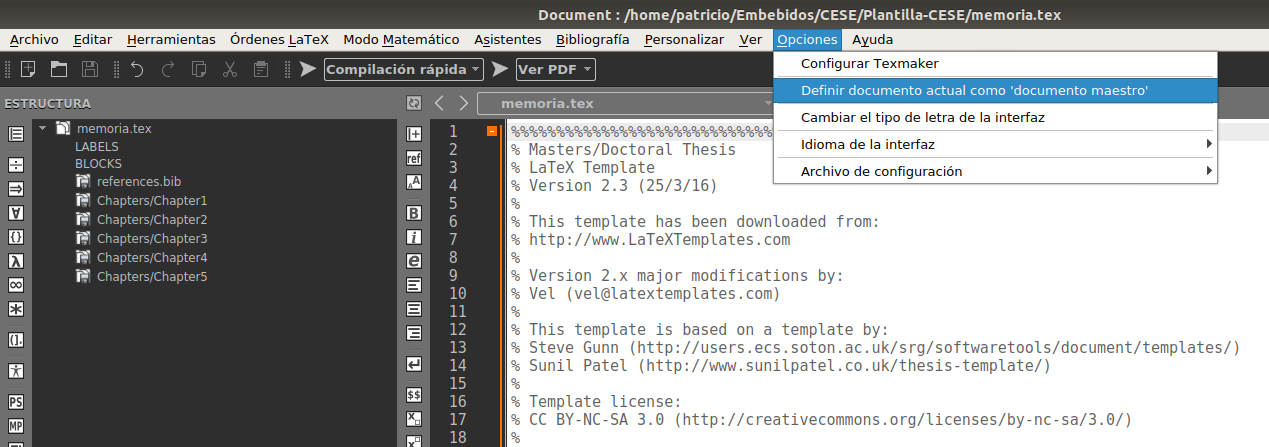
\includegraphics[width=\textwidth]{./Figures/docMaestro.png}
	\caption{Definir memoria.tex como documento maestro.}
	\label{fig:docMaestro}
\end{figure}

En el menú herramientas se encuentran las opciones de compilación.  Para producir un archivo PDF a partir de un archivo .tex se debe ejecutar PDFLaTeX (el shortcut es F6). Para incorporar nueva bibliografía se debe utilizar la opción BibTeX del mismo menú herramientas (el shortcut es F11).

Notar que para actualizar las tablas de contenidos se debe ejecutar PDFLaTeX dos veces.  Esto se debe a que es necesario actualizar algunos archivos auxiliares antes de obtener el resultado final.  En forma similar, para actualizar las referencias se debe ejecutar primero PDFLaTeX, después BibTeX y finalmente PDFLaTeX dos veces por idénticos motivos.

\section{Personalizando la plantilla, el archivo \file{memoria.tex}}
\label{sec:FillingFile}

Para personalizar la plantilla se debe incorporar la información propia en los distintos archivos \file{.tex}. 

Primero abrir \file{memoria.tex} con TexMaker (o el editor de su preferencia). Se debe ubicar dentro del archivo el bloque de código titulado \emph{INFORMACIÓN DE LA PORTADA} donde se deben incorporar los primeros datos personales con los que se construirá automáticamente la portada.


%----------------------------------------------------------------------------------------

\section{El código del archivo \file{memoria.tex} explicado}

El archivo \file{memoria.tex} contiene la estructura del documento y es el archivo de mayor jerarquía de la memoria.  Podría ser equiparable a la función \emph{main()} de un programa en C, o mejor dicho al archivo fuente .c donde se encuentra definida la función main().

La estructura básica de cualquier documento de \LaTeX{} comienza con la definición de clase del documento, es seguida por un preámbulo donde se pueden agregar funcionalidades con el uso de \texttt{paquetes} (equiparables a bibliotecas de C), y finalmente, termina con el cuerpo del documento, donde irá el contenido de la memoria.

\lstset{%
  basicstyle=\small\ttfamily,
  language=[LaTeX]{TeX}
}

\begin{lstlisting}
\documentclass{article}  <- Definicion de clase
\usepackage{listings}	 <- Preambulo

\begin{document}	 <- Comienzo del contenido propio 
	Hello world!
\end{document}
\end{lstlisting}


El archivo \file{memoria.tex} se encuentra densamente comentado para explicar qué páginas, secciones y elementos de formato está creando el código \LaTeX{} en cada línea. El código está dividido en bloques con nombres en mayúsculas para que resulte evidente qué es lo que hace esa porción de código en particular. Inicialmente puede parecer que hay mucho código \LaTeX{}, pero es principalmente código para dar formato a la memoria por lo que no requiere intervención del usuario de la plantilla.  Sí se deben personalizar con su información los bloques indicados como:

\begin{itemize}
	\item Informacion de la memoria
	\item Resumen
	\item Agradecimientos
	\item Dedicatoria
\end{itemize}

El índice de contenidos, las listas de figura de tablas se generan en forma automática y no requieren intervención ni edición manual por parte del usuario de la plantilla. 

En la parte final del documento se encuentran los capítulos y los apéndices.  Por defecto se incluyen los 5 capítulos propuestos que se encuentran en la carpeta /Chapters. Cada capítulo se debe escribir en un archivo .tex separado y se debe poner en la carpeta \emph{Chapters} con el nombre \file{Chapter1}, \file{Chapter2}, etc\ldots El código para incluir capítulos desde archivos externos se muestra a continuación.

\begin{verbatim}
	\include{Chapters/Chapter1}
	\include{Chapters/Chapter2} 
	\include{Chapters/Chapter3}
	\include{Chapters/Chapter4} 
	\include{Chapters/Chapter5} 
\end{verbatim}

Los apéndices también deben escribirse en archivos .tex separados, que se deben ubicar dentro de la carpeta \emph{Appendices}. Los apéndices vienen comentados por defecto con el caracter \code{\%} y para incluirlos simplemente se debe eliminar dicho caracter.

Finalmente, se encuentra el código para incluir la bibliografía en el documento final.  Este código tampoco debe modificarse. La metodología para trabajar las referencias bibliográficas se desarrolla en la sección \ref{sec:biblio}.
%----------------------------------------------------------------------------------------

\section{Bibliografía}
\label{sec:biblio}

Las opciones de formato de la bibliografía se controlan a través del paquete de latex \option{biblatex} que se incluye en la memoria en el archivo memoria.tex.  Estas opciones determinan cómo se generan las citas bibliográficas en el cuerpo del documento y cómo se genera la bibliografía al final de la memoria.

En el preámbulo se puede encontrar el código que incluye el paquete biblatex, que no requiere ninguna modificación del usuario de la plantilla, y que contiene las siguientes opciones:

\begin{lstlisting}
\usepackage[backend=bibtex,
	natbib=true, 
	style=numeric, 
	sorting=none]
{biblatex}
\end{lstlisting}

En el archivo \file{reference.bib} se encuentran las referencias bibliográficas que se pueden citar en el documento.  Para incorporar una nueva cita al documento lo primero es agregarla en este archivo con todos los campos necesario.  Todas las entradas bibliográficas comienzan con $@$ y una palabra que define el formato de la entrada.  Para cada formato existen campos obligatorios que deben completarse. No importa el orden en que las entradas estén definidas en el archivo .bib.  Tampoco es importante el orden en que estén definidos los campos de una entrada bibliográfica. A continuación se muestran algunos ejemplos:

\begin{lstlisting}
@ARTICLE{ARTICLE:1,
    AUTHOR="John Doe",
    TITLE="Title",
    JOURNAL="Journal",
    YEAR="2017",
}
\end{lstlisting}


\begin{lstlisting}
@BOOK{BOOK:1,
    AUTHOR="John Doe",
    TITLE="The Book without Title",
    PUBLISHER="Dummy Publisher",
    YEAR="2100",
}
\end{lstlisting}


\begin{lstlisting}
@INBOOK{BOOK:2,
    AUTHOR="John Doe",
    TITLE="The Book without Title",
    PUBLISHER="Dummy Publisher",
    YEAR="2100",
    PAGES="100-200",
}
\end{lstlisting}


\begin{lstlisting}
@MISC{WEBSITE:1,
    HOWPUBLISHED = "\url{http://example.com}",
    AUTHOR = "Intel",
    TITLE = "Example Website",
    MONTH = "12",
    YEAR = "1988",
    URLDATE = {2012-11-26}
}
\end{lstlisting}

Se debe notar que los nombres \emph{ARTICLE:1}, \emph{BOOK:1}, \emph{BOOK:2} y \emph{WEBSITE:1} son nombres de fantasía que le sirve al autor del documento para identificar la entrada. En este sentido, se podrían reemplazar por cualquier otro nombre.  Tampoco es necesario poner : seguido de un número, en los ejemplos sólo se incluye como un posible estilo para identificar las entradas.

La entradas se citan en el documento con el comando: 

\begin{verbatim}
\citep{nombre_de_la_entrada}
\end{verbatim}

Y cuando se usan, se muestran así: \citep{ARTICLE:1}, \citep{BOOK:1}, \citep{BOOK:2}, \citep{WEBSITE:1}.  Notar cómo se conforma la sección Bibliografía al final del documento. 

	\chapter{Introducción específica}

En este capítulo se presenta un resumen de los conceptos más relevantes acerca de la red TCN y su implementación en las formaciones de Trenes Argentinos, y se detallan las diferentes tecnologías utilizadas para el desarrollo del dispositivo de captura.

\section{La red TCN}

La red TCN es una combinación jerárquica de dos buses de datos en los que se transmite información dentro de una formación ferroviaria. El \textit{Multifunction Vehicle Bus} (MVB) interconecta los diferentes dispositivos presentes dentro de cada vehículo, y el \textit{Wire Train Bus} (WTB) interconecta los diferentes vehículos. Los componentes de la red TCN están estandarizados en la norma IEC 61375-1. En la figura~\ref{fig:tcn-mvb-wtb} se muestra un diagrama simplificado de la arquitectura TCN.

\begin{figure}[htbp]
	\centering
    {
        \fontfamily{phv}
        \fontsize{9pt}{9pt}\selectfont
        \input{./Figures/tcn-mvb-wtb.pdf_tex}
    }
	\caption[\textit{Wire Train Bus} y \textit{Multifunction Vehicle Bus}]{\textit{Wire Train Bus} y \textit{Multifunction Vehicle Bus}.\footnotemark}
    \label{fig:tcn-mvb-wtb}
\end{figure}
\footnotetext{Dibujo del tren por Freepik\\(\url{https://www.freepik.com/free-vector/collection-different-types-trains_1114167.htm})}

Dado que el dispositivo desarrollado se conecta al bus MVB, a continuación se exponen las características principales de este bus de comunicación.

\subsection{El bus MVB}

El bus MVB interconecta diferentes dispositivos ubicados en el mismo vehículo o en diferentes vehículos que no son separados con frecuencia. El MVB puede direccionar hasta 4095 dispositivos de distintos tipos, desde simples sensores y actuadores hasta equipos programables.

La estructura de MVB sigue el modelo OSI \cite{ISO7498-1}, que establece siete capas de abstracción en el proceso de transmisión de datos.
En las capas inferiores del protocolo MVB se establecen las características del medio físico y la estructura de las tramas y telegramas.
A continuación, se describen estos conceptos, que son los más relevantes para el desarrollo de este trabajo.

\subsection{Capa física}

El bus MVB ofrece tres opciones de medios físicos para la capa inferior:

\begin{itemize}
\item El medio \textit{Electrical Short Distance} (ESD), para distancias de hasta 20~m, que soporta hasta 32 dispositivos por segmento, con transceptores de tipo RS-485.
\item El medio \textit{Electrical Middle Distance} (EMD), para distancias de hasta 200~m, que soporta hasta  32 dispositivos por segmento, con transformadores y transceptores compatibles con la norma IEC 61158-2 \cite{iec61158_2}.
\item El medio \textit{Optical Glass Fibre} (OGF), para distancias de hasta 2000~m, y soporta conexiones punto a punto o subredes de topología tipo estrella.
\end{itemize}

Puede haber diferentes buses en un vehículo, interconectados mediante un \textit{gateway} al bus WTB.
También es posible que el bus MVB abarque más de un vehículo, y en este caso la norma recomienda el medio EMD.
Un ejemplo de esta configuración se ilustra en la figura~\ref{fig:emd-esd-wtb}.

\begin{figure}[htbp]
	\centering
    {
        \fontfamily{phv}
        \fontsize{9pt}{9pt}\selectfont
        \input{./Figures/medios.pdf_tex}
    }
	\caption[MVB abarcando tres vehículos]{MVB abarcando tres vehículos.}
    \label{fig:emd-esd-wtb}
\end{figure}

En la figura~\ref{fig:segmento} se ilustra un segmento EMD.
Cada dispositivo conectado a un segmento EMD tiene dos conectores D-sub de 9 pines (DE-9) que van, respectivamente, al dispositivo anterior y siguiente en el segmento. Los dispositivos en los extremos del segmento tienen un terminador.

\begin{figure}[htbp]
	\centering
    {
        \fontfamily{phv}
        \fontsize{9pt}{9pt}\selectfont
        \input{./Figures/segmento-emd.pdf_tex}
    }
	\caption[Un segmento EMD]{Un segmento EMD.}
    \label{fig:segmento}
\end{figure}

En la figura~\ref{fig:pines} se muestra la configuración de pines de los conectores.
La transmisión de la señal digital se realiza mediante la tensión diferencial entre los pares Data\_N y Data\_P. La norma permite que haya una única línea (A) o dos líneas (A y B) para proporcionar redundancia.

\begin{figure}[htbp]
	\centering
    {
        \fontfamily{phv}
        \fontsize{8pt}{8pt}\selectfont
        \input{./Figures/db9-emd.pdf_tex}
    }
	\caption[Configuración de pines del conector D-sub de 9 pines del medio EMD]{Configuración de pines del conector DE-9 del medio EMD. Se omite por simplicidad la interconexión de los pines 6 a 9, que se utilizan para los terminadores.}
    \label{fig:pines}
\end{figure}

\subsection{Tramas}
\label{sec:tramas}

Se denomina ``trama'' a un paquete de datos transmitido por un dispositivo.
En el bus MVB se transmiten dos tipos de tramas:

\begin{itemize}
\item La trama \textit{master}, que es transmitida únicamente por el dispositivo maestro del bus.
\item La trama \textit{slave}, que es transmitida por un dispositivo esclavo en respuesta a una trama \textit{master}.
\end{itemize}

Todos los medios MVB operan a una velocidad unificada de 1,5~Mbit/s.
La información se transmite utilizando una codificación Manchester, que combina en una única señal la información y el \textit{clock}.

La transmisión de una trama se compone de un delimitador inicial (SD) de 9 bits de duración, los datos de la trama, una secuencia de verificación (CS) de 8 bits y un delimitador final (ED) de 2 bits de duración.
En los datos de la trama y la secuencia de verificación, un ``1'' se transmite como una transición negativa en el medio de una celda de bit, y un ``0'' se transmite como una transición positiva.
Los delimitadores de inicio para las tramas \textit{master} y \textit{slave} son diferentes, y se denominan MSD y SSD.
En la figura~\ref{fig:manchester} se muestra a modo de ejemplo la transmisión de una trama \textit{master} en el medio EMD.

\begin{figure}[htbp]
	\centering
    {
        \fontfamily{phv}
        \fontsize{8pt}{8pt}\selectfont
        \input{./Figures/manchester.pdf_tex}
    }
	\caption[Transmisión de una trama master]{Transmisión de una trama \textit{master}.}
    \label{fig:manchester}
\end{figure}


\subsection{Telegramas}

Una secuencia de una trama \textit{master} seguida de una trama \textit{slave} conforman un telegrama, como se muestra en la figura~\ref{fig:telegrama}.

\begin{figure}[htbp]
	\centering
    {
        \fontfamily{phv}
        \fontsize{8pt}{8pt}\selectfont
        \input{./Figures/telegrama.pdf_tex}
    }
	\caption[Un telegrama MVB]{Un telegrama MVB.}
    \label{fig:telegrama}
\end{figure}

Las tramas \textit{master} tienen una longitud fija de 16 bits (sin contar los delimitadores), e incluyen:

\begin{itemize}
\item Un código de 4 bits llamado \texttt{F\_code}, que indica el tipo y tamaño de la trama \textit{slave} esperada a continuación.
\item Un campo de 12 bits, que puede contener una dirección de destino, o parámetros específicos al \texttt{F\_code}.
\end{itemize}

Todos los dispositivos conectados al bus decodifican la trama \textit{master}. El dispositivo encuestado luego responde con su trama \textit{slave}, que a su vez puede ser recibida por otros dispositivos.

\subsection{Variables}

Son de particular interés los telegramas con \texttt{F\_code} entre 0 y 4, que se denominan \texttt{Process\_Data}.
En este caso, el campo de 12 bits contiene una dirección lógica que hace referencia a un puerto.
Cada puerto está asociado unívocamente a una variable, que puede contener uno o más valores como la velocidad actual, la tensión de red, el estado de las puertas, etc.
Cada dispositivo \textit{slave} almacena uno o más puertos, y al ser encuestado responde con el valor actual de la variable correspondiente.

\section{Red TCN en las formaciones de Trenes Argentinos}

En la figura~\ref{fig:tms} se muestra un diagrama simplificado de la topología de la red TCN en una sección de 3 vehículos EMU de una formación de Trenes Argentinos. En el diagrama se observa que los buses MVB están implementados con el medio físico EMD.

\begin{figure}[htbp]
	\centering
    {
        \fontfamily{phv}
        \fontsize{8pt}{8pt}\selectfont
        \input{./Figures/tms.pdf_tex}
    }
	\caption[Topología de la red TCN en una formación de Trenes Argentinos]{Topología de la red TCN en una formación de Trenes Argentinos.}
    \label{fig:tms}
\end{figure}

\pagebreak

En la figura~\ref{fig:rcme} se muestra una fotografía de uno de los dispositivos presentes en la cabina del conductor de una formación de la línea Mitre. Se trata del módulo de comunicación RCMe, que controla las puertas, el sistema de aire acondicionado y el sistema de información al pasajero. En el panel frontal del módulo RCMe, los conectores DE-9 X1 y X2 (destacados en la figura) corresponden al bus MVB.

\begin{figure}[htbp]
	\centering
	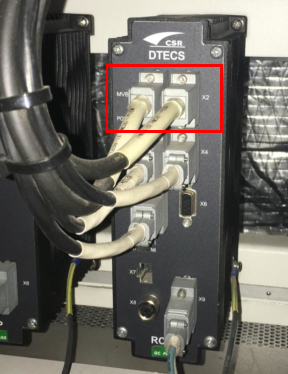
\includegraphics[width=0.5\textwidth]{./Figures/RCMe.pdf}
	\caption[El módulo de comunicación RCMe]{El módulo de comunicación RCMe presente en un EMU. Los dos conectores DE-9 destacados corresponden al bus MVB.}
    \label{fig:rcme}
\end{figure}

La pantalla HMI (\textit{Human Machine Interface}), también ubicada en la cabina del conductor, tiene un modo de operación que permite visualizar el valor de algunas variables que son transmitidas periódicamente en forma de \texttt{Process\_Data}. En la figura~\ref{fig:hmi} se puede observar que en el puerto 0 hay una variable de 16 bits cuyo valor binario actual es 1100 0001 0110 0101, o 33702 si se interpreta como un número decimal.

\begin{figure}[htbp]
	\centering
	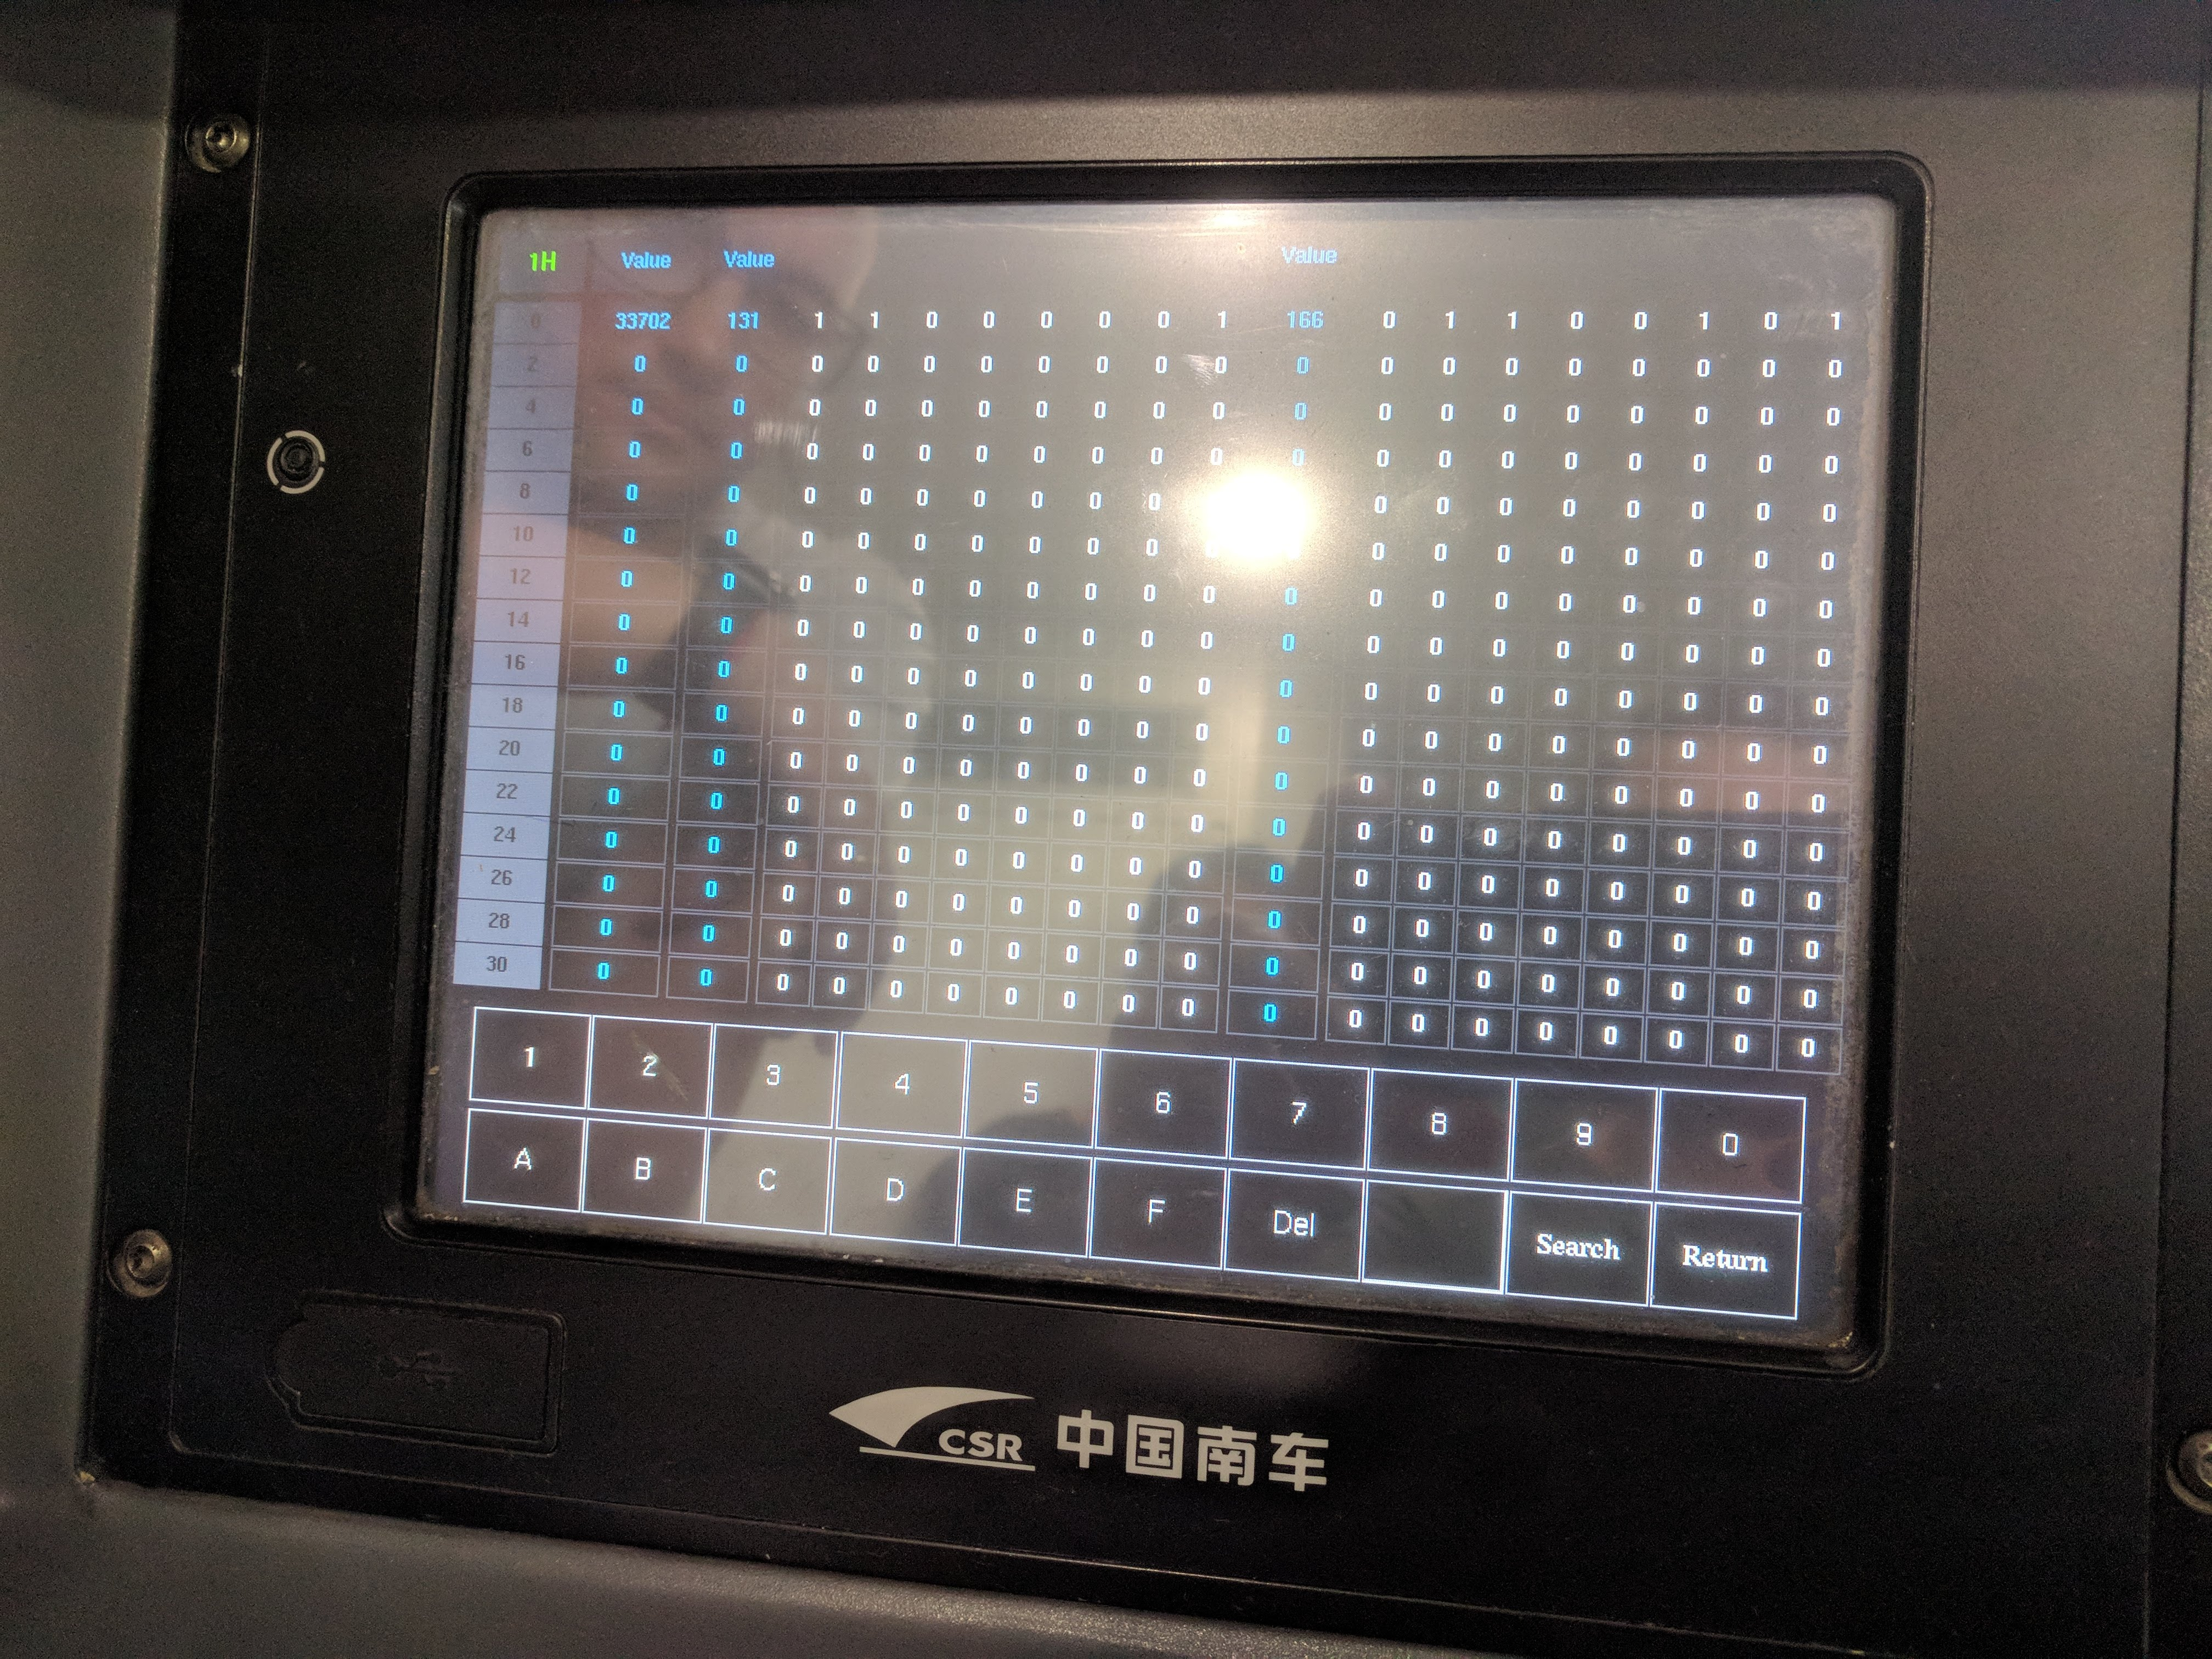
\includegraphics[width=1\textwidth]{./Figures/hmi.jpg}
	\caption[El HMI mostrando algunas variables]{El HMI mostrando algunas variables.}
    \label{fig:hmi}
\end{figure}

\section{Componentes del sistema}

A continuación, se describen las principales tecnologías utilizadas para el desarrollo del dispositivo de captura.

\subsection{EDU-CIAA}

La EDU-CIAA \cite{web:ciaa} es una plataforma de desarrollo de hardware libre basada en el microcontrolador NXP LPC4337 \cite{web:lpc4337} (dual core ARM Cortex-M4F y Cortex-M0), diseñada para la enseñanza de la programación y el desarrollo de sistemas embebidos en Argentina y otros países de habla hispana.
Esta placa cuenta con múltiples interfaces de entrada/salida, como puertos USB, Ethernet, CAN, UART, I²C, SPI, ADC y DAC.

La EDU-CIAA se utilizó para desarrollar un generador de señal MVB que permitió probar el funcionamiento del dispositivo de captura sin necesidad de conectarlo en una formación ferroviaria. El diseño del generador se describe en la sección \ref{sec:generador}.

\subsection{Raspberry Pi}

La Raspberry Pi \cite{web:rpi} es una computadora de placa única (SBC, por sus siglas en inglés) de bajo costo y tamaño reducido, diseñada por la \textit{Raspberry Pi Foundation} para promover la enseñanza de la informática básica en las escuelas y países en desarrollo.
Entre sus capacidades se encuentran el procesamiento de video en alta definición, conectividad inalámbrica y soporte para una gran cantidad de periféricos, lo que la convierte en una opción popular para una amplia gama de proyectos, desde la automatización del hogar hasta la robótica y la creación de servidores web.

El dispositivo de captura desarrollado en este trabajo está basado en la Raspberry Pi. Su diseño se describe en la sección \ref{sec:hardware}.

\subsection{Analizador lógico VKTECH y Sigrok}

El analizador lógico VKTECH \cite{vktech} es un dispositivo que permite capturar y analizar señales digitales en sistemas electrónicos. El dispositivo provee 8 canales que pueden capturar con una frecuencia de muestreo de hasta 24MHz, y cuenta con una interfaz USB 2.0 para conectar a una PC.

Sigrok \cite{sigrok} es un software libre y de código abierto que proporciona una plataforma para la adquisición y análisis de datos de múltiples tipos de instrumentos de medición, incluyendo analizadores lógicos, osciloscopios y multímetros. La herramienta es compatible con una amplia gama de dispositivos y marcas, lo que permite la integración de diferentes equipos y protocolos de comunicación en un solo entorno de software. Además, Sigrok ofrece una interfaz gráfica intuitiva y fácil de usar, así como una API para el desarrollo de aplicaciones personalizadas.

En este trabajo se utilizó el analizador lógico VKTECH y Sigrok en la fase de investigación, para realizar capturas del tráfico del bus MVB y analizarlas, como se menciona en las secciones \ref{sec:capturas} y \ref{sec:decodificacion}.

El dispositivo de captura desarrollado también utiliza el analizador lógico VKTECH y Sigrok para capturar el tráfico del bus en tiempo real, como se describe en las secciones \ref{sec:hardware} y  \ref{sec:software}.

\subsection{Python}

Python \cite{web:python} es un lenguaje de programación interpretado, de alto nivel y de propósito general. Está diseñado para ser fácil de aprender y cuenta con una sintaxis clara y legible.
Además tiene una amplia variedad de librerías y frameworks disponibles que permiten desarrollar aplicaciones en diferentes áreas, como ciencia de datos, inteligencia artificial, automatización y desarrollo web.

En este trabajo se utilizó el lenguaje Python en la fase de investigación, para decodificar las primeras capturas realizadas en la formación, como se describe en la sección \ref{sec:capturas}.

\subsection{Go}

Go \cite{web:go} es un lenguaje de programación de código abierto desarrollado por Google.
Se trata de un lenguaje de alto nivel, compilado, con tipos estáticos y recolector de basura.
Es sintácticamente similar al lenguaje C, pero se caracteriza por su enfoque en la concurrencia, la eficiencia y la simplicidad en la escritura de código.

Se utilizó el lenguaje Go para escribir el software del dispositivo de captura que corre en la Raspberry Pi, como se describe en la sección \ref{sec:software}.
 
	\chapter{Diseño e implementación}
\label{cap:DisenioImplementacion}

En este capítulo se presenta la arquitectura de hardware y software del dispositivo de captura, como así también del generador de señal MVB desarrollado para probar el dispositivo de captura sin necesidad de conectarlo en una formación ferroviaria.

\section{Arquitectura de hardware}
\label{sec:hardware}

Como se muestra en la figura~\ref{fig:conexion}, el dispositivo de captura tiene dos conectores DE-9 compatibles con el medio EMD. De esta manera se lo puede conectar a un segmento MVB entre dos dispositivos cualesquiera.

\begin{figure}[htbp]
	\centering
    {
        \fontfamily{phv}
        \fontsize{8pt}{8pt}\selectfont
        \input{./Figures/conexion.pdf_tex}
    }
	\caption{Conexión del dispositivo de captura en un segmento EMD.}
    \label{fig:conexion}
\end{figure}

En la figura~\ref{fig:bloques} se muestra un diagrama de la arquitectura del dispositivo de captura.
Se dejan en corto circuito las líneas de transmisión (ver figura~\ref{fig:pines}), de forma tal de que el dispositivo opere en forma pasiva. Salvando la impedancia que agrega a la línea, el dispositivo de captura es transparente para el resto de los dispositivos del segmento.
El dispositivo MAX485 \cite{max485} se utiliza para convertir la señal de entrada (par diferencial $-$5~V - +5~V) a una señal compatible para el analizador lógico VKTECH (0~V - +5~V). El analizador lógico se conecta a una Raspberry Pi mediante un puerto USB 2.0. La Raspberry Pi decodifica las tramas por software y almacena los datos capturados en una tarjeta de memoria. Mediante su interfaz Wi-Fi se puede conectar una PC (utilizando el protocolo SSH) para descargar las capturas, y también para visualizar el tráfico del bus MVB en tiempo real.

\begin{figure}[htbp]
	\centering
    {
        \fontfamily{phv}
        \fontsize{8pt}{8pt}\selectfont
        \input{./Figures/bloques.pdf_tex}
    }
	\caption{Arquitectura de hardware del dispositivo de captura.}
    \label{fig:bloques}
\end{figure}

En la figura~\ref{fig:esquematico} se muestra un diagrama esquemático con el detalle de las conexiones entre los diferentes componentes. En el diagrama se utiliza la etiqueta ``USB'' para representar la conexión a la Raspberry Pi, que no se muestra por simplicidad. Asimismo, la conexión ``VCC'' del MAX485 se conecta al pin número 2 del conector GPIO de la Raspberry Pi \cite{gpio}.

\begin{figure}[htbp]
	\centering
	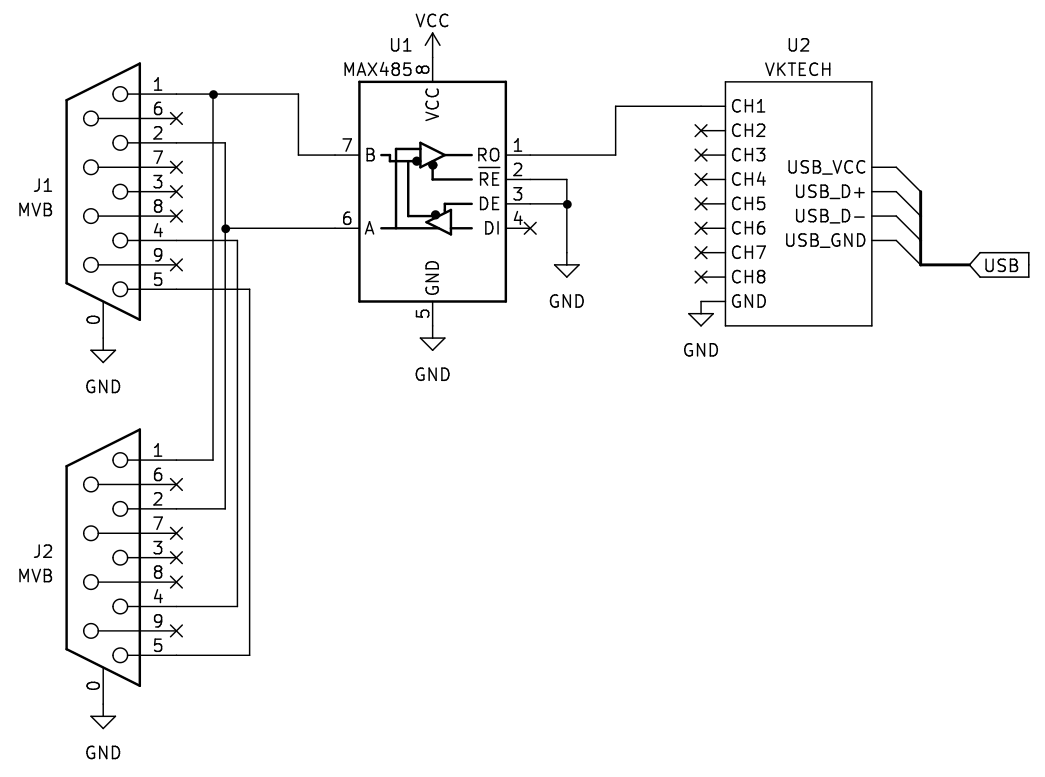
\includegraphics[width=1\textwidth]{./Figures/esquematico.png}
	\caption{Diagrama esquemático del dispositivo de captura.}
    \label{fig:esquematico}
\end{figure}

En la figura~\ref{fig:fotodispositivo} se muestra una foto del dispositivo de captura en construcción. Cabe aclarar que en el dispositivo hay cuatro MAX485 para permitir, en el futuro, capturar ambas líneas A y B del segmento EMD, o bien capturar dos o más segmentos diferentes. En esta primera versión del dispositivo se utiliza solo uno de los MAX485.

\begin{figure}[htbp]
	\centering
	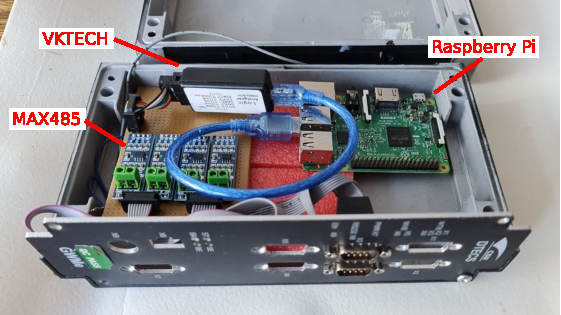
\includegraphics[width=1\textwidth]{./Figures/foto-dispositivo.pdf}
	\caption{Foto del dispositivo de captura en construcción.}
    \label{fig:fotodispositivo}
\end{figure}

\section{Arquitectura de software}
\label{sec:software}

Como se ve en la figura~\ref{fig:bloques}, a la Raspberry Pi entra la señal digital capturada por el analizador lógico en tiempo real, mediante la interfaz USB. Para recibir esta señal se utiliza Sigrok, invocándolo de la siguiente manera:

\begin{lstlisting}
sigrok-cli -d fx2lafw --continuous --config samplerate=12m
           --channels D0 -O binary
\end{lstlisting}

Este comando recibe la señal del VKTECH en la interfaz USB, muestrea la señal digital con una frecuencia de 12 MHz y produce como salida un flujo de datos que se puede redireccionar a un archivo o a un \textit{pipe} de Unix.
Por cada muestra capturada, se emite un byte en el que el bit menos significativo es 0 o 1 dependiendo de si la señal lógica capturada es baja o alta.
De esta forma, el flujo de datos tiene un ancho de banda de 12 MB/s, aunque solo se usa uno de los 8 bits de cada byte.
En la figura~\ref{fig:sigrok} se muestra un ejemplo del flujo de datos producido por Sigrok.

\begin{figure}[htbp]
	\centering
    {
        \fontfamily{phv}
        \fontsize{9pt}{9pt}\selectfont
        \input{./Figures/sigrok.pdf_tex}
    }
	\caption{Flujo de datos producido por Sigrok.}
    \label{fig:sigrok}
\end{figure}

Sería posible bajar la frecuencia de captura a 6 MHz, pero no menos ya que el protocolo MVB transmite la señal a 1,5 Mbit/s en codificación Manchester.
Para lograr una captura suficientemente confiable se necesita que la frecuencia de muestreo sea de al menos 6 MHz.
La frecuencia elegida de 12 MHz ofrece un buen balance entre confiabilidad y eficiencia en espacio.

\pagebreak

El flujo de datos producido por Sigrok se redirecciona mediante un \textit{pipe} de Unix a un software programado en lenguaje Go. Como se muestra en la figura~\ref{fig:capas-software}, la decodificación se realiza en tres capas de procesamiento:

\begin{enumerate}
\item La capa inferior (\texttt{MVBStream}) lee el flujo de datos byte por byte y ofrece funcionalidades tales como leer muestras individualmente, esperar hasta la siguiente transición de estado (alto-bajo o bajo-alto), esperar una cantidad de tiempo, etc.
\item La capa intermedia (\texttt{MVBDecoder}) identifica las tramas MVB y por cada telegrama produce un evento (\texttt{Event}).
\item La capa superior recibe los eventos y los procesa según el modo de operación del software. Se ofrecen dos modos de operación:
    \begin{itemize}
        \item En el modo interactivo, el software presenta una interfaz de usuario en la que se muestra el tráfico MVB en tiempo real. En la figura~\ref{fig:interactivo} se muestra una captura de pantalla del modo interactivo.
        \item En el modo de almacenamiento, el software permite almacenar la evolución histórica de una o más variables de importancia.
    \end{itemize}
\end{enumerate}

\begin{figure}[htbp]
	\centering
    {
        \fontfamily{phv}
        \fontsize{9pt}{9pt}\selectfont
        \input{./Figures/capas-software.pdf_tex}
    }
	\caption{Capas de procesamiento del software de captura.}
    \label{fig:capas-software}
\end{figure}

\begin{figure}[htbp]
	\centering
	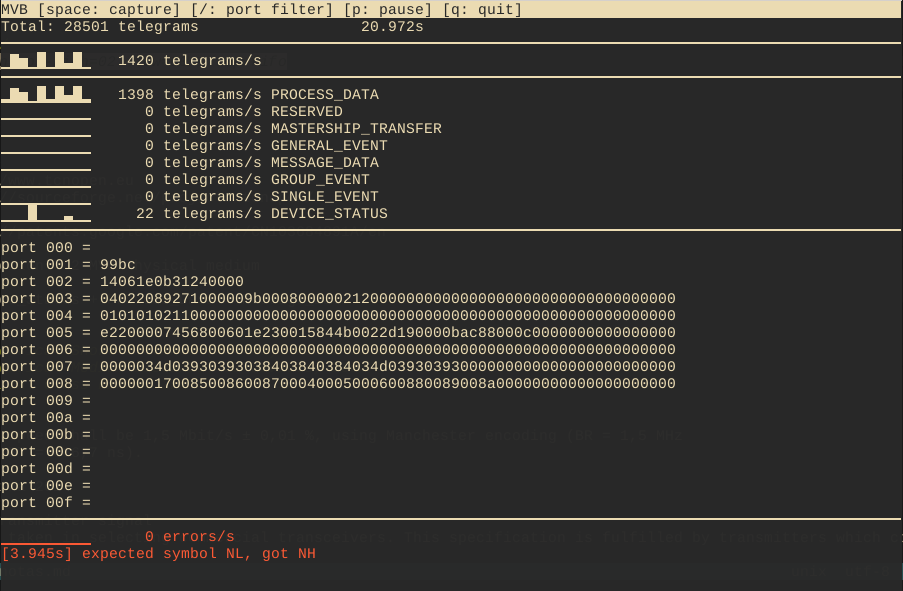
\includegraphics[width=1\textwidth]{./Figures/modo-interactivo.png}
	\caption{Modo interactivo del software de captura.}
    \label{fig:interactivo}
\end{figure}

El código fuente de este programa está disponible en la plataforma Github \cite{mvbparse-go}.
En el archivo \texttt{README.md} se muestran más detalles acerca de los diferentes modos de funcionamiento.

\section{Dispositivo generador de señal}
\label{sec:generador}

	\chapter{Ensayos y resultados}

\label{cap:EnsayosResultados}

En este capítulo se describe la fase de investigación previa al desarrollo del dispositivo de captura, junto con las pruebas realizadas para validar su correcto funcionamiento, tanto en un entorno de laboratorio como en una formación de Trenes Argentinos.

\section{Capturas del tráfico de la red en una formación}
\label{sec:capturas}

Como parte de la etapa de investigación, se realizaron visitas a los talleres de Trenes Argentinos en Victoria y Castelar, coordinadas respectivamente por Sergio Dieleke (Laboratorio Electrónico, Subgerencia de Material Rodante Línea Mitre) y Bruno Pilato (Laboratorio de Electrónica de Castelar, Línea Sarmiento).
El objetivo principal de estas visitas fue tomar capturas del tráfico del bus MVB, para ganar conocimiento acerca del estándar TCN y de la implementación particular en las EMU de Trenes Argentinos.

Para tomar las capturas se conectó un MAX485 y un analizador lógico VKTECH entre dos dispositivos MVB.
Se utilizó una PC para controlar el VKTECH y almacenar las diferentes capturas.
También se utilizó un osciloscopio para verificar que la señal capturada tuviera las características esperadas.
En la figura~\ref{fig:banco-capturas} se muestra un diagrama de bloques del banco de medición.
En las figuras~\ref{fig:foto-banco-capturas} y \ref{fig:osciloscopio} se muestra una fotografía del banco de medición y un detalle de la señal capturada en el osciloscopio.

% video con la secuencia https://drive.google.com/drive/folders/1I-V33ElLX13Iy0YliUeojRwYFQKuucAO
\begin{figure}[htbp]
	\centering
    {
        \fontfamily{phv}
        \fontsize{9pt}{9pt}\selectfont
        \input{./Figures/banco-captura.pdf_tex}
    }
	\caption{Banco de medición utilizado para tomar las capturas.}
    \label{fig:banco-capturas}
\end{figure}

\begin{figure}[htbp]
	\centering
	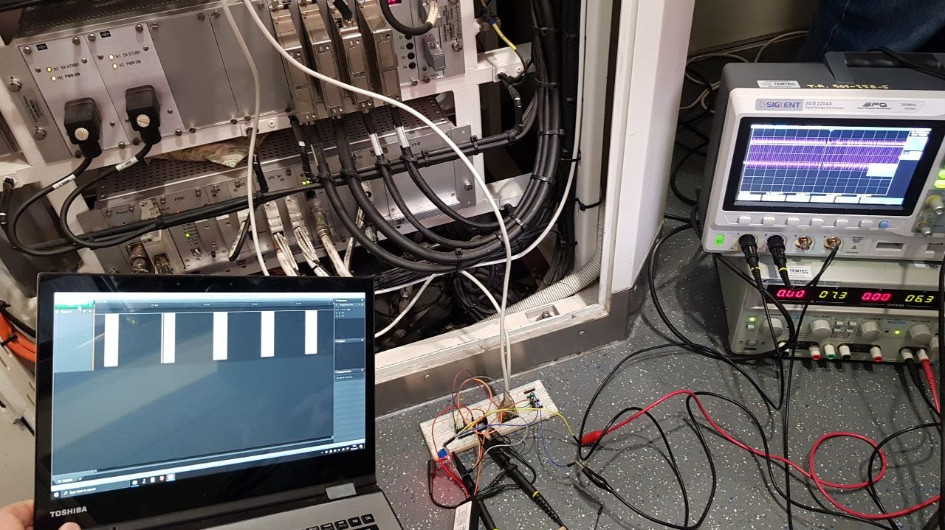
\includegraphics[width=\textwidth]{./Figures/foto-capturas.jpg}
	\caption{Fotografía del banco de medición utilizado para tomar las capturas.}
    \label{fig:foto-banco-capturas}
\end{figure}

\begin{figure}[htbp]
	\centering
	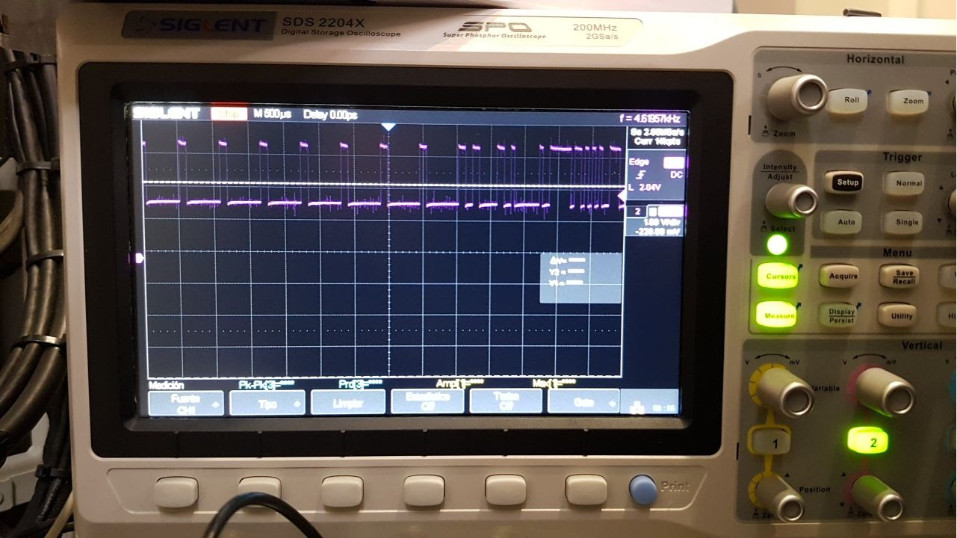
\includegraphics[width=\textwidth]{./Figures/osciloscopio.jpg}
	\caption{Señal MVB capturada en el osciloscopio.}
    \label{fig:osciloscopio}
\end{figure}

Se tomaron varias capturas de un minuto de duración del tráfico del bus MVB, con el banco de medición conectado en diferentes puntos del segmento.
Durante la toma de las capturas se efectuó el procedimiento de encendido de la red y una secuencia de pasos tales como tomar cabina, abrir y cerrar puertas, cambio de marcha, etc., de forma tal de generar tráfico en la red y así poder identificar las variables asociadas a estos eventos.

En la figura~\ref{fig:pulseview} se muestra una visualización de una de las capturas.
En la parte superior se observa que en los primeros 10 ms se transmitieron 10 telegramas, aunque el nivel de detalle no es suficiente para discernir el formato de las tramas.
En la parte inferior se amplía la visualización de uno de los telegramas, donde se puede apreciar en detalle las tramas \textit{master} y \textit{slave}, descriptas en la sección~\ref{sec:tramas}.
Estas visualizaciones se obtuvieron utilizando el software PulseView, que es parte del proyecto Sigrok.

\begin{figure}[htbp!]
	\centering
    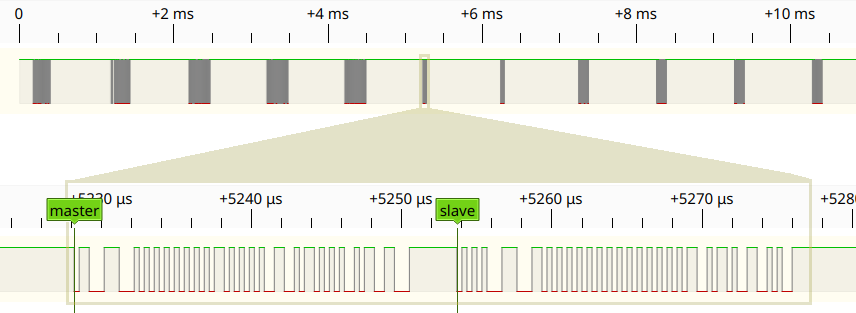
\includegraphics[width=\textwidth]{./Figures/pulseview.png}
    \caption{Visualización de una de las capturas realizadas.}
    \label{fig:pulseview}
\end{figure}

\section{Decodificación de las capturas}
\label{sec:decodificacion}

El siguiente objetivo en la etapa de investigación fue decodificar la información de las tramas capturadas. Para ello se desarrolló un programa en lenguaje Python que toma como entrada una captura en formato binario (un byte por muestra, como se describe en la sección \ref{sec:software}) y produce como salida un reporte de la información decodificada.

El software se compone de dos programas. El primero de ellos, \texttt{mvb\_signal.py}, toma como entrada una captura en formato binario, decodifica los datos codificados en Manchester, y produce como salida un archivo en formato CSV en el que cada línea representa un telegrama y tiene la forma \texttt{<tiempo>,\allowbreak <master>,\allowbreak <slave>}, donde \texttt{<tiempo>} es la marca de tiempo en segundos del telegrama, y \texttt{<master>} y \texttt{<slave>} es el contenido de las tramas en formato hexadecimal, sin incluir los delimitadores y las secuencias de verificación. En el código~\ref{cod:mvbsignal} se muestra un ejemplo de ejecución, en el que se procesa una captura que contiene 4 telegramas.

\begin{lstlisting}[label=cod:mvbsignal,caption=Ejemplo de ejecución de \texttt{mvb\_signal.py}.,float=htbp]
$ python3 mvb_signal.py < captura1.bin
0.0001,4390d6,971e0000008214
0.0011,431bf7,30000f
0.0021,000134,971e07
0.0022,4010c5,04004830580048
\end{lstlisting}

La salida de \texttt{mvb\_signal.py} se puede redireccionar mediante un \textit{pipe} al segundo programa, \texttt{mvbparse.py}, que interpreta la información de las tramas según el protocolo MVB y produce un reporte de la evolución de cada una de las variables identificadas. En el código~\ref{cod:mvbparse} se muestra un ejemplo de ejecución de \texttt{mvbparse.py}.

\begin{lstlisting}[label=cod:mvbparse,caption=Ejemplo de ejecución de \texttt{mvbparse.py}.,float=htbp,basicstyle=\footnotesize\ttfamily]
$ python3 mvb_signal.py < captura2.bin | python3 mvbparse.py
 [[port='0x31b'] [n=   12] [
                  t=  0.001s  0x30000f0c0110000000000000000011a8]],
 [[port='0x353'] [n=    3] [
                  t=  0.212s  0xe2036aa0000000000
                  t=  0.471s  0xe2036ba0000000000
                  t=  0.730s  0xe2036da0000000000]],
\end{lstlisting}

La salida de ejemplo de \texttt{mvbparse.py} indica que se identificaron dos variables, en los puertos \texttt{0x31b} y \texttt{0x353}.
La primera variable fue transmitida en total 12 veces, con un valor de 16 bytes. Se transmitió por primera vez en la marca temporal $0{,}001$ s, con un valor de 16 bytes, y luego se transmitió 11 veces más con el mismo valor.
La variable en el puerto \texttt{0x353} fue transmitida en total 3 veces con un valor de 8 bytes diferente cada vez.

Dado que durante la captura se realizaron diferentes acciones según se mencionó en la sección \ref{sec:capturas} (tomar cabina, abrir y cerrar puertas, etc.), fue posible, analizando la salida producida por el programa, detectar cuáles son las variables que cambian en función del momento en que estas acciones fueron efectuadas. En la figura~\ref{fig:analisis-captura} se muestra, por ejemplo, que la variable en el puerto \texttt{0x1b2} se modifica cada vez que se realizan las acciones de tomar cabina, y seleccionar, abrir y cerrar las puertas.

\begin{figure}[htbp]
	\centering
	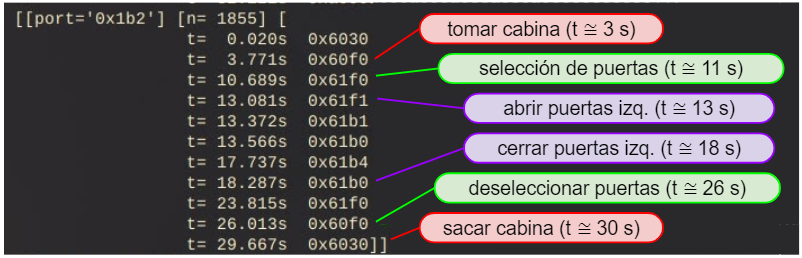
\includegraphics[width=\textwidth]{./Figures/analisis-captura.png}
	\caption[Resultado del análisis de una de las capturas.]{Resultado del análisis de una de las capturas.}
    \label{fig:analisis-captura}
\end{figure}

El software de decodificación está disponible en la plataforma Github \cite{mvbparse-py}. El desarrollo de este prototipo no solo sirvió para proporcionar información valiosa acerca del funcionamiento del bus MVB en las formaciones de Trenes Argentinos, sino también brindó la experiencia necesaria para el posterior desarrollo del software de captura descripto en la sección \ref{sec:software}.

\section{Pruebas del dispositivo de captura}

A continuación se describen los diferentes tipos de pruebas efectuadas para verificar el correcto funcionamiento del dispositivo de captura.

\subsection{Prueba del software de captura}

Para probar el correcto funcionamiento del software de captura (descripto en la sección \ref{sec:software}) se utilizaron las capturas tomadas en la formación ferroviaria (ver sección \ref{sec:capturas}).

Para ejecutar esta prueba se ejecuta el software pasándole como entrada el contenido de una de las capturas en lugar del flujo de datos en tiempo real. Para ello, en una consola se crea un FIFO y se lo alimenta con el contenido de la captura en un ciclo infinito. Se utiliza el comando \texttt{pv} \cite{pv} para limitar el ancho de banda a 12 MB/s:

\begin{lstlisting}
$ mkfifo /tmp/fifo
$ while cat captura.bin; do :; done | pv -L 12M > /tmp/fifo
\end{lstlisting}

En otra consola se ejecuta el software de captura tomando el FIFO como entrada.

\begin{lstlisting}
$ go run cmd/main.go </tmp/fifo
\end{lstlisting}

Esta técnica permite utilizar el software en una PC, como si estuviera conectado al bus MVB.
De esta manera se pudo probar todas sus funcionalidades, tanto en el modo interactivo como en el modo de captura.

\subsection{Prueba de integración de hardware}

% 28 oct 2021?
% 24 nov 2021?

El siguiente paso fue efectuar una prueba de integración del software de captura recibiendo el flujo de datos del VKTECH en tiempo real.
Para ello se utilizó el generador de señal MVB descripto en la sección \ref{sec:generador}, en una configuración como se muestra en la figura~\ref{fig:generador}.
En la figura~\ref{fig:educiaa+vktech} se muestra el banco de medición utilizado en esta prueba.

Esta prueba permitió verificar que es posible utilizar el VKTECH para recibir el flujo de datos en tiempo real.
La prueba se realizó con el software de captura corriendo tanto en una PC como en una Raspberry Pi.

\begin{figure}[htbp]
	\centering
	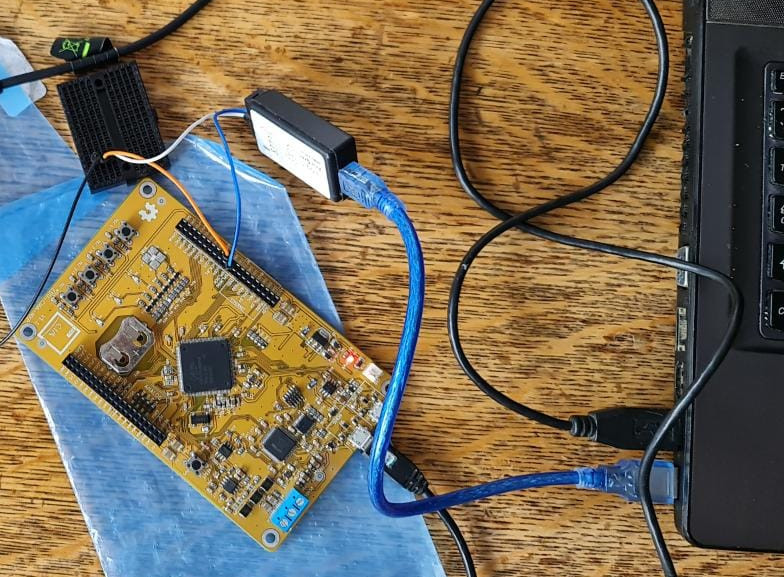
\includegraphics[width=\textwidth]{./Figures/educiaa+vktech.jpg}
	\caption{Banco de medición de la prueba utilizando el generador de señal MVB.}
    \label{fig:educiaa+vktech}
\end{figure}


\subsection{Prueba en una formación ferroviaria}

% 3 dic 2021 (PC)

% 6 ene 2022? (RPI)

La última prueba que se efectuó fue con el dispositivo de captura conectado en el bus MVB en una formación de Trenes Argentinos, como se muestra en la figura~\ref{fig:conexion}.
Se verificó que la conexión del dispositivo de captura no afectó al correcto funcionamiento del resto de los dispositivos conectados en el bus MVB. Cabe destacar que esta prueba se realizó en una formación detenida.

En la figura~\ref{fig:disp-captura-ssh} se muestra una fotografía de la pantalla de la PC utilizada durante la sesión de prueba. En la pantalla se observan dos consolas conectadas a la Raspberry Pi mediante el protocolo SSH. En la consola de la izquierda se ejecuta el comando \texttt{sigrok-cli} para recibir el flujo de datos del VKTECH en tiempo real. En la consola de la derecha se ejecuta el software de captura en modo interactivo.

\begin{figure}[htbp]
	\centering
	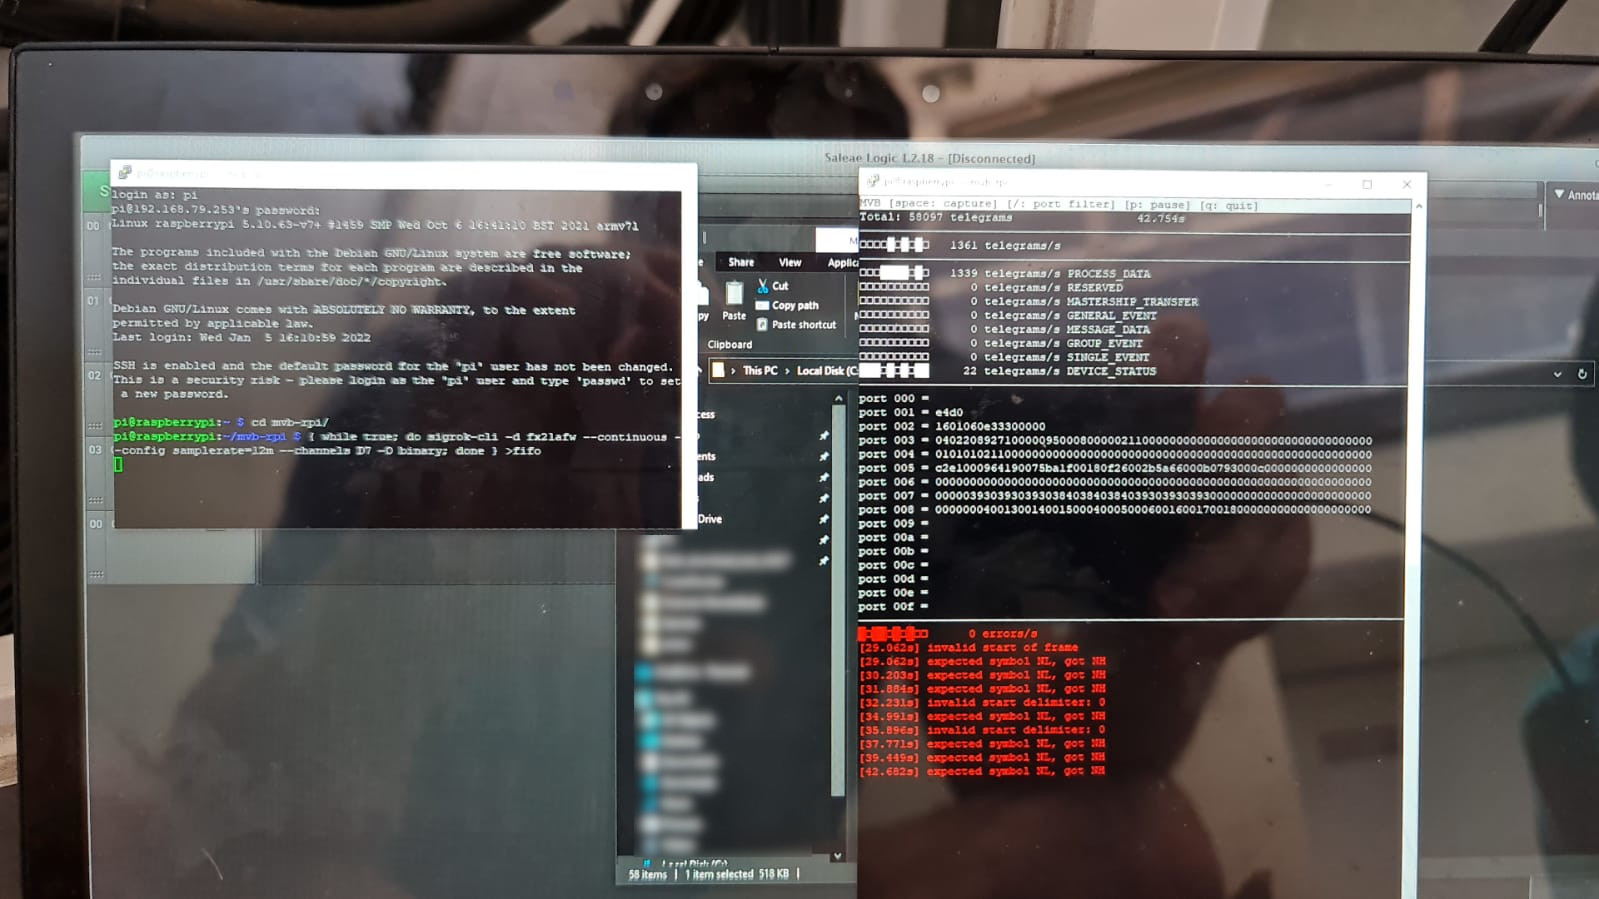
\includegraphics[width=\textwidth]{./Figures/disp-captura-ssh.jpg}
	\caption{Sesión de prueba del dispositivo de captura.}
    \label{fig:disp-captura-ssh}
\end{figure}
 
	% Chapter Template

\chapter{Conclusiones} % Main chapter title

\label{Chapter5} % Change X to a consecutive number; for referencing this chapter elsewhere, use \ref{ChapterX}


%----------------------------------------------------------------------------------------

%----------------------------------------------------------------------------------------
%	SECTION 1
%----------------------------------------------------------------------------------------

\section{Conclusiones generales }

La idea de esta sección es resaltar cuáles son los principales aportes del trabajo realizado y cómo se podría continuar. Debe ser especialmente breve y concisa. Es buena idea usar un listado para enumerar los logros obtenidos.

Algunas preguntas que pueden servir para completar este capítulo:

\begin{itemize}
\item ¿Cuál es el grado de cumplimiento de los requerimientos?
\item ¿Cuán fielmente se puedo seguir la planificación original (cronograma incluido)?
\item ¿Se manifestó algunos de los riesgos identificados en la planificación? ¿Fue efectivo el plan de mitigación? ¿Se debió aplicar alguna otra acción no contemplada previamente?
\item Si se debieron hacer modificaciones a lo planificado ¿Cuáles fueron las causas y los efectos?
\item ¿Qué técnicas resultaron útiles para el desarrollo del proyecto y cuáles no tanto?
\end{itemize}


%----------------------------------------------------------------------------------------
%	SECTION 2
%----------------------------------------------------------------------------------------
\section{Próximos pasos}

Acá se indica cómo se podría continuar el trabajo más adelante.
 
\end{verbatim}

Los apéndices también deben escribirse en archivos .tex separados, que se deben ubicar dentro de la carpeta \emph{Appendices}. Los apéndices vienen comentados por defecto con el caracter \code{\%} y para incluirlos simplemente se debe eliminar dicho caracter.

Finalmente, se encuentra el código para incluir la bibliografía en el documento final.  Este código tampoco debe modificarse. La metodología para trabajar las referencias bibliográficas se desarrolla en la sección \ref{sec:biblio}.
%----------------------------------------------------------------------------------------

\section{Bibliografía}
\label{sec:biblio}

Las opciones de formato de la bibliografía se controlan a través del paquete de latex \option{biblatex} que se incluye en la memoria en el archivo memoria.tex.  Estas opciones determinan cómo se generan las citas bibliográficas en el cuerpo del documento y cómo se genera la bibliografía al final de la memoria.

En el preámbulo se puede encontrar el código que incluye el paquete biblatex, que no requiere ninguna modificación del usuario de la plantilla, y que contiene las siguientes opciones:

\begin{lstlisting}
\usepackage[backend=bibtex,
	natbib=true, 
	style=numeric, 
	sorting=none]
{biblatex}
\end{lstlisting}

En el archivo \file{reference.bib} se encuentran las referencias bibliográficas que se pueden citar en el documento.  Para incorporar una nueva cita al documento lo primero es agregarla en este archivo con todos los campos necesario.  Todas las entradas bibliográficas comienzan con $@$ y una palabra que define el formato de la entrada.  Para cada formato existen campos obligatorios que deben completarse. No importa el orden en que las entradas estén definidas en el archivo .bib.  Tampoco es importante el orden en que estén definidos los campos de una entrada bibliográfica. A continuación se muestran algunos ejemplos:

\begin{lstlisting}
@ARTICLE{ARTICLE:1,
    AUTHOR="John Doe",
    TITLE="Title",
    JOURNAL="Journal",
    YEAR="2017",
}
\end{lstlisting}


\begin{lstlisting}
@BOOK{BOOK:1,
    AUTHOR="John Doe",
    TITLE="The Book without Title",
    PUBLISHER="Dummy Publisher",
    YEAR="2100",
}
\end{lstlisting}


\begin{lstlisting}
@INBOOK{BOOK:2,
    AUTHOR="John Doe",
    TITLE="The Book without Title",
    PUBLISHER="Dummy Publisher",
    YEAR="2100",
    PAGES="100-200",
}
\end{lstlisting}


\begin{lstlisting}
@MISC{WEBSITE:1,
    HOWPUBLISHED = "\url{http://example.com}",
    AUTHOR = "Intel",
    TITLE = "Example Website",
    MONTH = "12",
    YEAR = "1988",
    URLDATE = {2012-11-26}
}
\end{lstlisting}

Se debe notar que los nombres \emph{ARTICLE:1}, \emph{BOOK:1}, \emph{BOOK:2} y \emph{WEBSITE:1} son nombres de fantasía que le sirve al autor del documento para identificar la entrada. En este sentido, se podrían reemplazar por cualquier otro nombre.  Tampoco es necesario poner : seguido de un número, en los ejemplos sólo se incluye como un posible estilo para identificar las entradas.

La entradas se citan en el documento con el comando: 

\begin{verbatim}
\citep{nombre_de_la_entrada}
\end{verbatim}

Y cuando se usan, se muestran así: \citep{ARTICLE:1}, \citep{BOOK:1}, \citep{BOOK:2}, \citep{WEBSITE:1}.  Notar cómo se conforma la sección Bibliografía al final del documento. 

	\chapter{Introducción específica}

En este capítulo se presenta un resumen de los conceptos más relevantes acerca de la red TCN y su implementación en las formaciones de Trenes Argentinos, y se detallan las diferentes tecnologías utilizadas para el desarrollo del dispositivo de captura.

\section{La red TCN}

La red TCN es una combinación jerárquica de dos buses de datos en los que se transmite información dentro de una formación ferroviaria. El \textit{Multifunction Vehicle Bus} (MVB) interconecta los diferentes dispositivos presentes dentro de cada vehículo, y el \textit{Wire Train Bus} (WTB) interconecta los diferentes vehículos. Los componentes de la red TCN están estandarizados en la norma IEC 61375-1. En la figura~\ref{fig:tcn-mvb-wtb} se muestra un diagrama simplificado de la arquitectura TCN.

\begin{figure}[htbp]
	\centering
    {
        \fontfamily{phv}
        \fontsize{9pt}{9pt}\selectfont
        \input{./Figures/tcn-mvb-wtb.pdf_tex}
    }
	\caption[\textit{Wire Train Bus} y \textit{Multifunction Vehicle Bus}]{\textit{Wire Train Bus} y \textit{Multifunction Vehicle Bus}.\footnotemark}
    \label{fig:tcn-mvb-wtb}
\end{figure}
\footnotetext{Dibujo del tren por Freepik\\(\url{https://www.freepik.com/free-vector/collection-different-types-trains_1114167.htm})}

Dado que el dispositivo desarrollado se conecta al bus MVB, a continuación se exponen las características principales de este bus de comunicación.

\subsection{El bus MVB}

El bus MVB interconecta diferentes dispositivos ubicados en el mismo vehículo o en diferentes vehículos que no son separados con frecuencia. El MVB puede direccionar hasta 4095 dispositivos de distintos tipos, desde simples sensores y actuadores hasta equipos programables.

La estructura de MVB sigue el modelo OSI \cite{ISO7498-1}, que establece siete capas de abstracción en el proceso de transmisión de datos.
En las capas inferiores del protocolo MVB se establecen las características del medio físico y la estructura de las tramas y telegramas.
A continuación, se describen estos conceptos, que son los más relevantes para el desarrollo de este trabajo.

\subsection{Capa física}

El bus MVB ofrece tres opciones de medios físicos para la capa inferior:

\begin{itemize}
\item El medio \textit{Electrical Short Distance} (ESD), para distancias de hasta 20~m, que soporta hasta 32 dispositivos por segmento, con transceptores de tipo RS-485.
\item El medio \textit{Electrical Middle Distance} (EMD), para distancias de hasta 200~m, que soporta hasta  32 dispositivos por segmento, con transformadores y transceptores compatibles con la norma IEC 61158-2 \cite{iec61158_2}.
\item El medio \textit{Optical Glass Fibre} (OGF), para distancias de hasta 2000~m, y soporta conexiones punto a punto o subredes de topología tipo estrella.
\end{itemize}

Puede haber diferentes buses en un vehículo, interconectados mediante un \textit{gateway} al bus WTB.
También es posible que el bus MVB abarque más de un vehículo, y en este caso la norma recomienda el medio EMD.
Un ejemplo de esta configuración se ilustra en la figura~\ref{fig:emd-esd-wtb}.

\begin{figure}[htbp]
	\centering
    {
        \fontfamily{phv}
        \fontsize{9pt}{9pt}\selectfont
        \input{./Figures/medios.pdf_tex}
    }
	\caption[MVB abarcando tres vehículos]{MVB abarcando tres vehículos.}
    \label{fig:emd-esd-wtb}
\end{figure}

En la figura~\ref{fig:segmento} se ilustra un segmento EMD.
Cada dispositivo conectado a un segmento EMD tiene dos conectores D-sub de 9 pines (DE-9) que van, respectivamente, al dispositivo anterior y siguiente en el segmento. Los dispositivos en los extremos del segmento tienen un terminador.

\begin{figure}[htbp]
	\centering
    {
        \fontfamily{phv}
        \fontsize{9pt}{9pt}\selectfont
        \input{./Figures/segmento-emd.pdf_tex}
    }
	\caption[Un segmento EMD]{Un segmento EMD.}
    \label{fig:segmento}
\end{figure}

En la figura~\ref{fig:pines} se muestra la configuración de pines de los conectores.
La transmisión de la señal digital se realiza mediante la tensión diferencial entre los pares Data\_N y Data\_P. La norma permite que haya una única línea (A) o dos líneas (A y B) para proporcionar redundancia.

\begin{figure}[htbp]
	\centering
    {
        \fontfamily{phv}
        \fontsize{8pt}{8pt}\selectfont
        \input{./Figures/db9-emd.pdf_tex}
    }
	\caption[Configuración de pines del conector D-sub de 9 pines del medio EMD]{Configuración de pines del conector DE-9 del medio EMD. Se omite por simplicidad la interconexión de los pines 6 a 9, que se utilizan para los terminadores.}
    \label{fig:pines}
\end{figure}

\subsection{Tramas}
\label{sec:tramas}

Se denomina ``trama'' a un paquete de datos transmitido por un dispositivo.
En el bus MVB se transmiten dos tipos de tramas:

\begin{itemize}
\item La trama \textit{master}, que es transmitida únicamente por el dispositivo maestro del bus.
\item La trama \textit{slave}, que es transmitida por un dispositivo esclavo en respuesta a una trama \textit{master}.
\end{itemize}

Todos los medios MVB operan a una velocidad unificada de 1,5~Mbit/s.
La información se transmite utilizando una codificación Manchester, que combina en una única señal la información y el \textit{clock}.

La transmisión de una trama se compone de un delimitador inicial (SD) de 9 bits de duración, los datos de la trama, una secuencia de verificación (CS) de 8 bits y un delimitador final (ED) de 2 bits de duración.
En los datos de la trama y la secuencia de verificación, un ``1'' se transmite como una transición negativa en el medio de una celda de bit, y un ``0'' se transmite como una transición positiva.
Los delimitadores de inicio para las tramas \textit{master} y \textit{slave} son diferentes, y se denominan MSD y SSD.
En la figura~\ref{fig:manchester} se muestra a modo de ejemplo la transmisión de una trama \textit{master} en el medio EMD.

\begin{figure}[htbp]
	\centering
    {
        \fontfamily{phv}
        \fontsize{8pt}{8pt}\selectfont
        \input{./Figures/manchester.pdf_tex}
    }
	\caption[Transmisión de una trama master]{Transmisión de una trama \textit{master}.}
    \label{fig:manchester}
\end{figure}


\subsection{Telegramas}

Una secuencia de una trama \textit{master} seguida de una trama \textit{slave} conforman un telegrama, como se muestra en la figura~\ref{fig:telegrama}.

\begin{figure}[htbp]
	\centering
    {
        \fontfamily{phv}
        \fontsize{8pt}{8pt}\selectfont
        \input{./Figures/telegrama.pdf_tex}
    }
	\caption[Un telegrama MVB]{Un telegrama MVB.}
    \label{fig:telegrama}
\end{figure}

Las tramas \textit{master} tienen una longitud fija de 16 bits (sin contar los delimitadores), e incluyen:

\begin{itemize}
\item Un código de 4 bits llamado \texttt{F\_code}, que indica el tipo y tamaño de la trama \textit{slave} esperada a continuación.
\item Un campo de 12 bits, que puede contener una dirección de destino, o parámetros específicos al \texttt{F\_code}.
\end{itemize}

Todos los dispositivos conectados al bus decodifican la trama \textit{master}. El dispositivo encuestado luego responde con su trama \textit{slave}, que a su vez puede ser recibida por otros dispositivos.

\subsection{Variables}

Son de particular interés los telegramas con \texttt{F\_code} entre 0 y 4, que se denominan \texttt{Process\_Data}.
En este caso, el campo de 12 bits contiene una dirección lógica que hace referencia a un puerto.
Cada puerto está asociado unívocamente a una variable, que puede contener uno o más valores como la velocidad actual, la tensión de red, el estado de las puertas, etc.
Cada dispositivo \textit{slave} almacena uno o más puertos, y al ser encuestado responde con el valor actual de la variable correspondiente.

\section{Red TCN en las formaciones de Trenes Argentinos}

En la figura~\ref{fig:tms} se muestra un diagrama simplificado de la topología de la red TCN en una sección de 3 vehículos EMU de una formación de Trenes Argentinos. En el diagrama se observa que los buses MVB están implementados con el medio físico EMD.

\begin{figure}[htbp]
	\centering
    {
        \fontfamily{phv}
        \fontsize{8pt}{8pt}\selectfont
        \input{./Figures/tms.pdf_tex}
    }
	\caption[Topología de la red TCN en una formación de Trenes Argentinos]{Topología de la red TCN en una formación de Trenes Argentinos.}
    \label{fig:tms}
\end{figure}

\pagebreak

En la figura~\ref{fig:rcme} se muestra una fotografía de uno de los dispositivos presentes en la cabina del conductor de una formación de la línea Mitre. Se trata del módulo de comunicación RCMe, que controla las puertas, el sistema de aire acondicionado y el sistema de información al pasajero. En el panel frontal del módulo RCMe, los conectores DE-9 X1 y X2 (destacados en la figura) corresponden al bus MVB.

\begin{figure}[htbp]
	\centering
	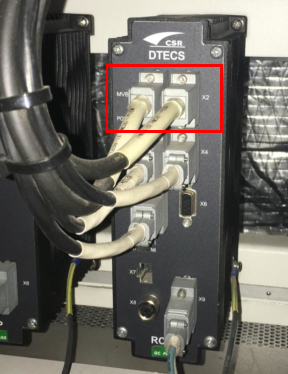
\includegraphics[width=0.5\textwidth]{./Figures/RCMe.pdf}
	\caption[El módulo de comunicación RCMe]{El módulo de comunicación RCMe presente en un EMU. Los dos conectores DE-9 destacados corresponden al bus MVB.}
    \label{fig:rcme}
\end{figure}

La pantalla HMI (\textit{Human Machine Interface}), también ubicada en la cabina del conductor, tiene un modo de operación que permite visualizar el valor de algunas variables que son transmitidas periódicamente en forma de \texttt{Process\_Data}. En la figura~\ref{fig:hmi} se puede observar que en el puerto 0 hay una variable de 16 bits cuyo valor binario actual es 1100 0001 0110 0101, o 33702 si se interpreta como un número decimal.

\begin{figure}[htbp]
	\centering
	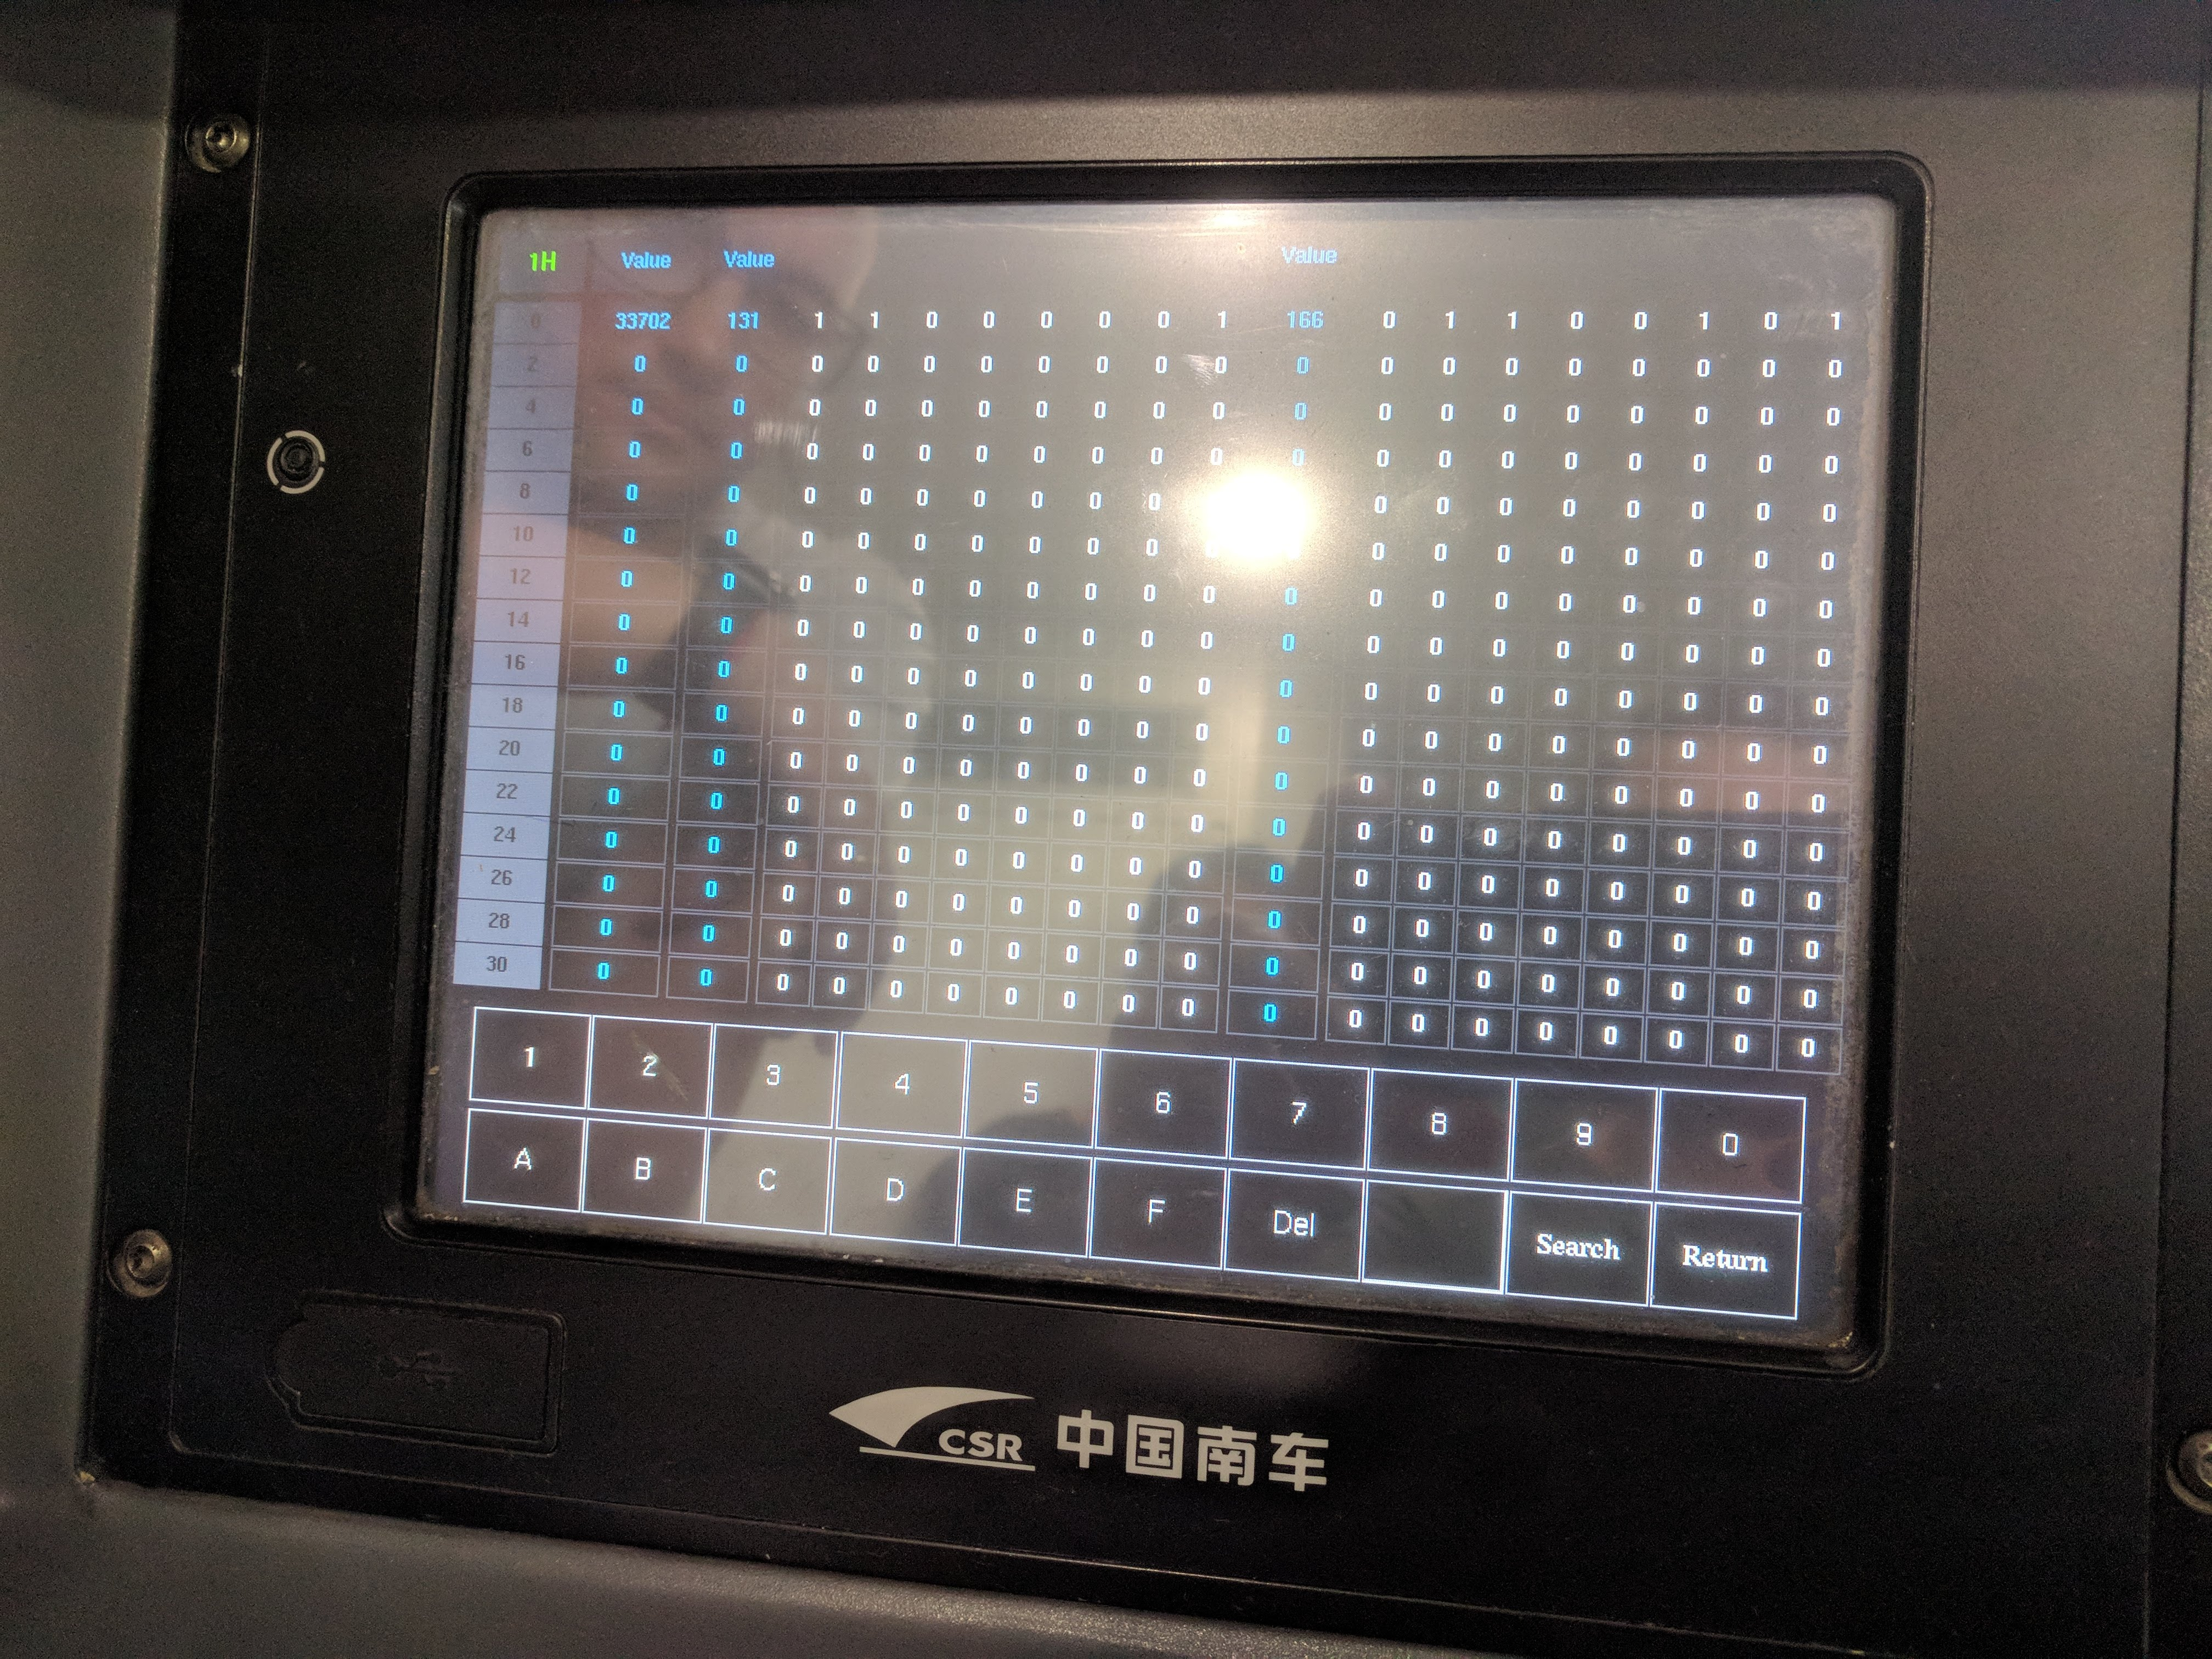
\includegraphics[width=1\textwidth]{./Figures/hmi.jpg}
	\caption[El HMI mostrando algunas variables]{El HMI mostrando algunas variables.}
    \label{fig:hmi}
\end{figure}

\section{Componentes del sistema}

A continuación, se describen las principales tecnologías utilizadas para el desarrollo del dispositivo de captura.

\subsection{EDU-CIAA}

La EDU-CIAA \cite{web:ciaa} es una plataforma de desarrollo de hardware libre basada en el microcontrolador NXP LPC4337 \cite{web:lpc4337} (dual core ARM Cortex-M4F y Cortex-M0), diseñada para la enseñanza de la programación y el desarrollo de sistemas embebidos en Argentina y otros países de habla hispana.
Esta placa cuenta con múltiples interfaces de entrada/salida, como puertos USB, Ethernet, CAN, UART, I²C, SPI, ADC y DAC.

La EDU-CIAA se utilizó para desarrollar un generador de señal MVB que permitió probar el funcionamiento del dispositivo de captura sin necesidad de conectarlo en una formación ferroviaria. El diseño del generador se describe en la sección \ref{sec:generador}.

\subsection{Raspberry Pi}

La Raspberry Pi \cite{web:rpi} es una computadora de placa única (SBC, por sus siglas en inglés) de bajo costo y tamaño reducido, diseñada por la \textit{Raspberry Pi Foundation} para promover la enseñanza de la informática básica en las escuelas y países en desarrollo.
Entre sus capacidades se encuentran el procesamiento de video en alta definición, conectividad inalámbrica y soporte para una gran cantidad de periféricos, lo que la convierte en una opción popular para una amplia gama de proyectos, desde la automatización del hogar hasta la robótica y la creación de servidores web.

El dispositivo de captura desarrollado en este trabajo está basado en la Raspberry Pi. Su diseño se describe en la sección \ref{sec:hardware}.

\subsection{Analizador lógico VKTECH y Sigrok}

El analizador lógico VKTECH \cite{vktech} es un dispositivo que permite capturar y analizar señales digitales en sistemas electrónicos. El dispositivo provee 8 canales que pueden capturar con una frecuencia de muestreo de hasta 24MHz, y cuenta con una interfaz USB 2.0 para conectar a una PC.

Sigrok \cite{sigrok} es un software libre y de código abierto que proporciona una plataforma para la adquisición y análisis de datos de múltiples tipos de instrumentos de medición, incluyendo analizadores lógicos, osciloscopios y multímetros. La herramienta es compatible con una amplia gama de dispositivos y marcas, lo que permite la integración de diferentes equipos y protocolos de comunicación en un solo entorno de software. Además, Sigrok ofrece una interfaz gráfica intuitiva y fácil de usar, así como una API para el desarrollo de aplicaciones personalizadas.

En este trabajo se utilizó el analizador lógico VKTECH y Sigrok en la fase de investigación, para realizar capturas del tráfico del bus MVB y analizarlas, como se menciona en las secciones \ref{sec:capturas} y \ref{sec:decodificacion}.

El dispositivo de captura desarrollado también utiliza el analizador lógico VKTECH y Sigrok para capturar el tráfico del bus en tiempo real, como se describe en las secciones \ref{sec:hardware} y  \ref{sec:software}.

\subsection{Python}

Python \cite{web:python} es un lenguaje de programación interpretado, de alto nivel y de propósito general. Está diseñado para ser fácil de aprender y cuenta con una sintaxis clara y legible.
Además tiene una amplia variedad de librerías y frameworks disponibles que permiten desarrollar aplicaciones en diferentes áreas, como ciencia de datos, inteligencia artificial, automatización y desarrollo web.

En este trabajo se utilizó el lenguaje Python en la fase de investigación, para decodificar las primeras capturas realizadas en la formación, como se describe en la sección \ref{sec:capturas}.

\subsection{Go}

Go \cite{web:go} es un lenguaje de programación de código abierto desarrollado por Google.
Se trata de un lenguaje de alto nivel, compilado, con tipos estáticos y recolector de basura.
Es sintácticamente similar al lenguaje C, pero se caracteriza por su enfoque en la concurrencia, la eficiencia y la simplicidad en la escritura de código.

Se utilizó el lenguaje Go para escribir el software del dispositivo de captura que corre en la Raspberry Pi, como se describe en la sección \ref{sec:software}.
 
	\chapter{Diseño e implementación}
\label{cap:DisenioImplementacion}

En este capítulo se presenta la arquitectura de hardware y software del dispositivo de captura, como así también del generador de señal MVB desarrollado para probar el dispositivo de captura sin necesidad de conectarlo en una formación ferroviaria.

\section{Arquitectura de hardware}
\label{sec:hardware}

Como se muestra en la figura~\ref{fig:conexion}, el dispositivo de captura tiene dos conectores DE-9 compatibles con el medio EMD. De esta manera se lo puede conectar a un segmento MVB entre dos dispositivos cualesquiera.

\begin{figure}[htbp]
	\centering
    {
        \fontfamily{phv}
        \fontsize{8pt}{8pt}\selectfont
        \input{./Figures/conexion.pdf_tex}
    }
	\caption{Conexión del dispositivo de captura en un segmento EMD.}
    \label{fig:conexion}
\end{figure}

En la figura~\ref{fig:bloques} se muestra un diagrama de la arquitectura del dispositivo de captura.
Se dejan en corto circuito las líneas de transmisión (ver figura~\ref{fig:pines}), de forma tal de que el dispositivo opere en forma pasiva. Salvando la impedancia que agrega a la línea, el dispositivo de captura es transparente para el resto de los dispositivos del segmento.
El dispositivo MAX485 \cite{max485} se utiliza para convertir la señal de entrada (par diferencial $-$5~V - +5~V) a una señal compatible para el analizador lógico VKTECH (0~V - +5~V). El analizador lógico se conecta a una Raspberry Pi mediante un puerto USB 2.0. La Raspberry Pi decodifica las tramas por software y almacena los datos capturados en una tarjeta de memoria. Mediante su interfaz Wi-Fi se puede conectar una PC (utilizando el protocolo SSH) para descargar las capturas, y también para visualizar el tráfico del bus MVB en tiempo real.

\begin{figure}[htbp]
	\centering
    {
        \fontfamily{phv}
        \fontsize{8pt}{8pt}\selectfont
        \input{./Figures/bloques.pdf_tex}
    }
	\caption{Arquitectura de hardware del dispositivo de captura.}
    \label{fig:bloques}
\end{figure}

En la figura~\ref{fig:esquematico} se muestra un diagrama esquemático con el detalle de las conexiones entre los diferentes componentes. En el diagrama se utiliza la etiqueta ``USB'' para representar la conexión a la Raspberry Pi, que no se muestra por simplicidad. Asimismo, la conexión ``VCC'' del MAX485 se conecta al pin número 2 del conector GPIO de la Raspberry Pi \cite{gpio}.

\begin{figure}[htbp]
	\centering
	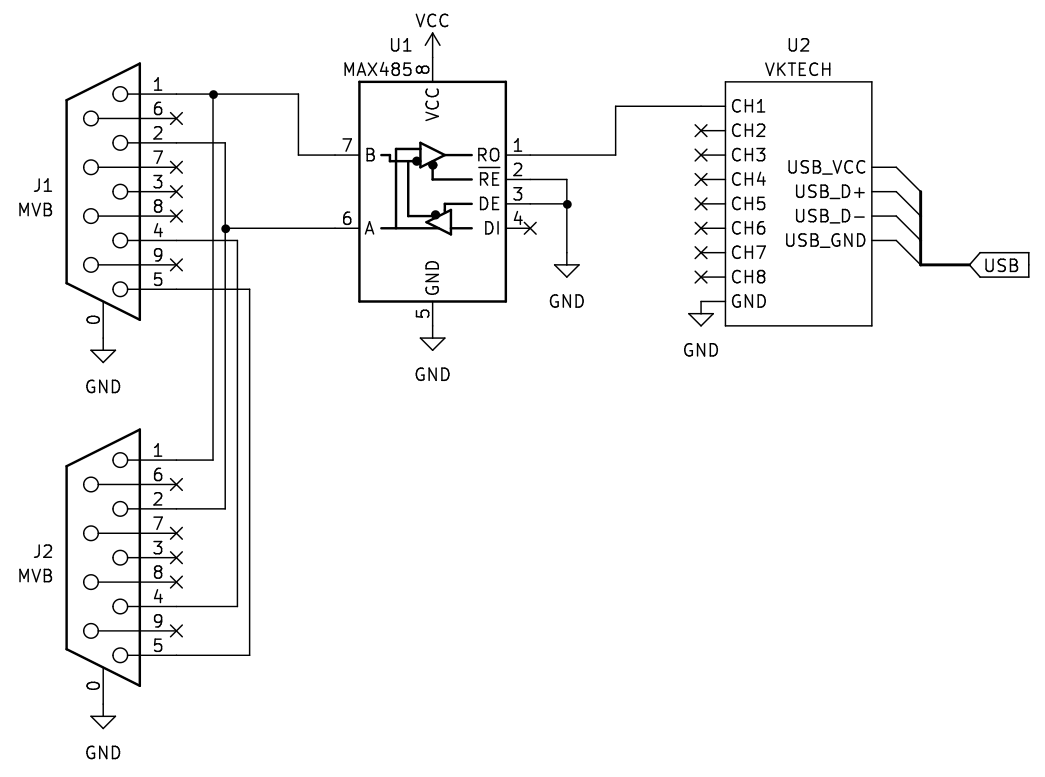
\includegraphics[width=1\textwidth]{./Figures/esquematico.png}
	\caption{Diagrama esquemático del dispositivo de captura.}
    \label{fig:esquematico}
\end{figure}

En la figura~\ref{fig:fotodispositivo} se muestra una foto del dispositivo de captura en construcción. Cabe aclarar que en el dispositivo hay cuatro MAX485 para permitir, en el futuro, capturar ambas líneas A y B del segmento EMD, o bien capturar dos o más segmentos diferentes. En esta primera versión del dispositivo se utiliza solo uno de los MAX485.

\begin{figure}[htbp]
	\centering
	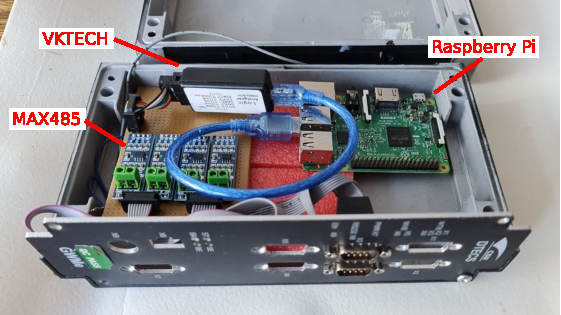
\includegraphics[width=1\textwidth]{./Figures/foto-dispositivo.pdf}
	\caption{Foto del dispositivo de captura en construcción.}
    \label{fig:fotodispositivo}
\end{figure}

\section{Arquitectura de software}
\label{sec:software}

Como se ve en la figura~\ref{fig:bloques}, a la Raspberry Pi entra la señal digital capturada por el analizador lógico en tiempo real, mediante la interfaz USB. Para recibir esta señal se utiliza Sigrok, invocándolo de la siguiente manera:

\begin{lstlisting}
sigrok-cli -d fx2lafw --continuous --config samplerate=12m
           --channels D0 -O binary
\end{lstlisting}

Este comando recibe la señal del VKTECH en la interfaz USB, muestrea la señal digital con una frecuencia de 12 MHz y produce como salida un flujo de datos que se puede redireccionar a un archivo o a un \textit{pipe} de Unix.
Por cada muestra capturada, se emite un byte en el que el bit menos significativo es 0 o 1 dependiendo de si la señal lógica capturada es baja o alta.
De esta forma, el flujo de datos tiene un ancho de banda de 12 MB/s, aunque solo se usa uno de los 8 bits de cada byte.
En la figura~\ref{fig:sigrok} se muestra un ejemplo del flujo de datos producido por Sigrok.

\begin{figure}[htbp]
	\centering
    {
        \fontfamily{phv}
        \fontsize{9pt}{9pt}\selectfont
        \input{./Figures/sigrok.pdf_tex}
    }
	\caption{Flujo de datos producido por Sigrok.}
    \label{fig:sigrok}
\end{figure}

Sería posible bajar la frecuencia de captura a 6 MHz, pero no menos ya que el protocolo MVB transmite la señal a 1,5 Mbit/s en codificación Manchester.
Para lograr una captura suficientemente confiable se necesita que la frecuencia de muestreo sea de al menos 6 MHz.
La frecuencia elegida de 12 MHz ofrece un buen balance entre confiabilidad y eficiencia en espacio.

\pagebreak

El flujo de datos producido por Sigrok se redirecciona mediante un \textit{pipe} de Unix a un software programado en lenguaje Go. Como se muestra en la figura~\ref{fig:capas-software}, la decodificación se realiza en tres capas de procesamiento:

\begin{enumerate}
\item La capa inferior (\texttt{MVBStream}) lee el flujo de datos byte por byte y ofrece funcionalidades tales como leer muestras individualmente, esperar hasta la siguiente transición de estado (alto-bajo o bajo-alto), esperar una cantidad de tiempo, etc.
\item La capa intermedia (\texttt{MVBDecoder}) identifica las tramas MVB y por cada telegrama produce un evento (\texttt{Event}).
\item La capa superior recibe los eventos y los procesa según el modo de operación del software. Se ofrecen dos modos de operación:
    \begin{itemize}
        \item En el modo interactivo, el software presenta una interfaz de usuario en la que se muestra el tráfico MVB en tiempo real. En la figura~\ref{fig:interactivo} se muestra una captura de pantalla del modo interactivo.
        \item En el modo de almacenamiento, el software permite almacenar la evolución histórica de una o más variables de importancia.
    \end{itemize}
\end{enumerate}

\begin{figure}[htbp]
	\centering
    {
        \fontfamily{phv}
        \fontsize{9pt}{9pt}\selectfont
        \input{./Figures/capas-software.pdf_tex}
    }
	\caption{Capas de procesamiento del software de captura.}
    \label{fig:capas-software}
\end{figure}

\begin{figure}[htbp]
	\centering
	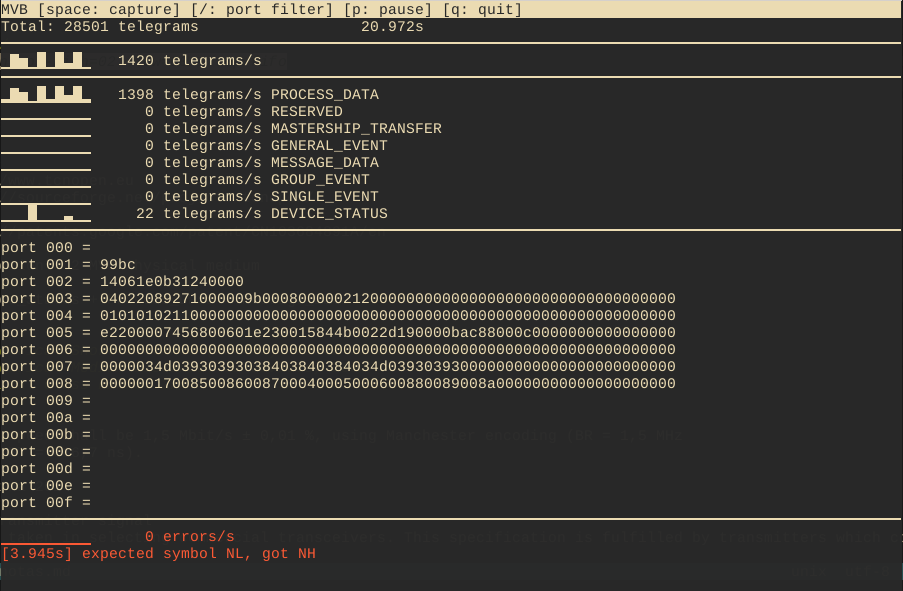
\includegraphics[width=1\textwidth]{./Figures/modo-interactivo.png}
	\caption{Modo interactivo del software de captura.}
    \label{fig:interactivo}
\end{figure}

El código fuente de este programa está disponible en la plataforma Github \cite{mvbparse-go}.
En el archivo \texttt{README.md} se muestran más detalles acerca de los diferentes modos de funcionamiento.

\section{Dispositivo generador de señal}
\label{sec:generador}

	\chapter{Ensayos y resultados}

\label{cap:EnsayosResultados}

En este capítulo se describe la fase de investigación previa al desarrollo del dispositivo de captura, junto con las pruebas realizadas para validar su correcto funcionamiento, tanto en un entorno de laboratorio como en una formación de Trenes Argentinos.

\section{Capturas del tráfico de la red en una formación}
\label{sec:capturas}

Como parte de la etapa de investigación, se realizaron visitas a los talleres de Trenes Argentinos en Victoria y Castelar, coordinadas respectivamente por Sergio Dieleke (Laboratorio Electrónico, Subgerencia de Material Rodante Línea Mitre) y Bruno Pilato (Laboratorio de Electrónica de Castelar, Línea Sarmiento).
El objetivo principal de estas visitas fue tomar capturas del tráfico del bus MVB, para ganar conocimiento acerca del estándar TCN y de la implementación particular en las EMU de Trenes Argentinos.

Para tomar las capturas se conectó un MAX485 y un analizador lógico VKTECH entre dos dispositivos MVB.
Se utilizó una PC para controlar el VKTECH y almacenar las diferentes capturas.
También se utilizó un osciloscopio para verificar que la señal capturada tuviera las características esperadas.
En la figura~\ref{fig:banco-capturas} se muestra un diagrama de bloques del banco de medición.
En las figuras~\ref{fig:foto-banco-capturas} y \ref{fig:osciloscopio} se muestra una fotografía del banco de medición y un detalle de la señal capturada en el osciloscopio.

% video con la secuencia https://drive.google.com/drive/folders/1I-V33ElLX13Iy0YliUeojRwYFQKuucAO
\begin{figure}[htbp]
	\centering
    {
        \fontfamily{phv}
        \fontsize{9pt}{9pt}\selectfont
        \input{./Figures/banco-captura.pdf_tex}
    }
	\caption{Banco de medición utilizado para tomar las capturas.}
    \label{fig:banco-capturas}
\end{figure}

\begin{figure}[htbp]
	\centering
	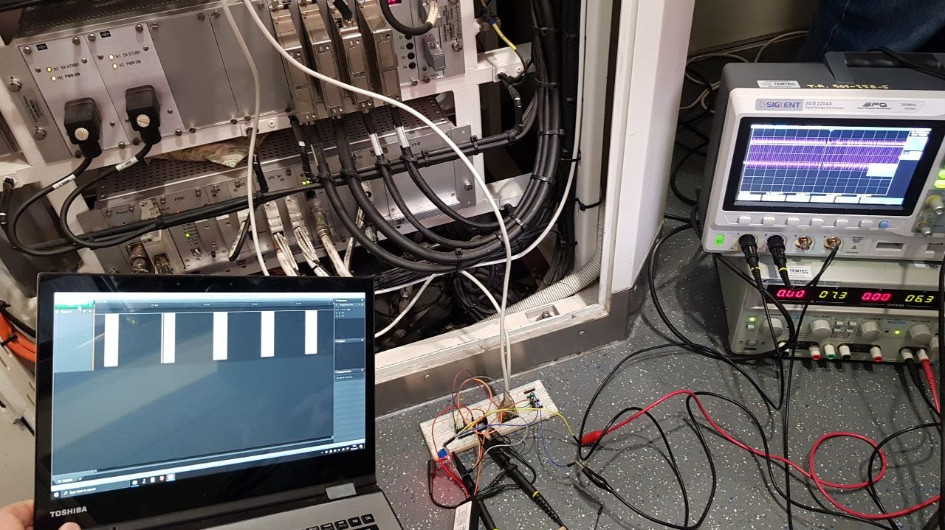
\includegraphics[width=\textwidth]{./Figures/foto-capturas.jpg}
	\caption{Fotografía del banco de medición utilizado para tomar las capturas.}
    \label{fig:foto-banco-capturas}
\end{figure}

\begin{figure}[htbp]
	\centering
	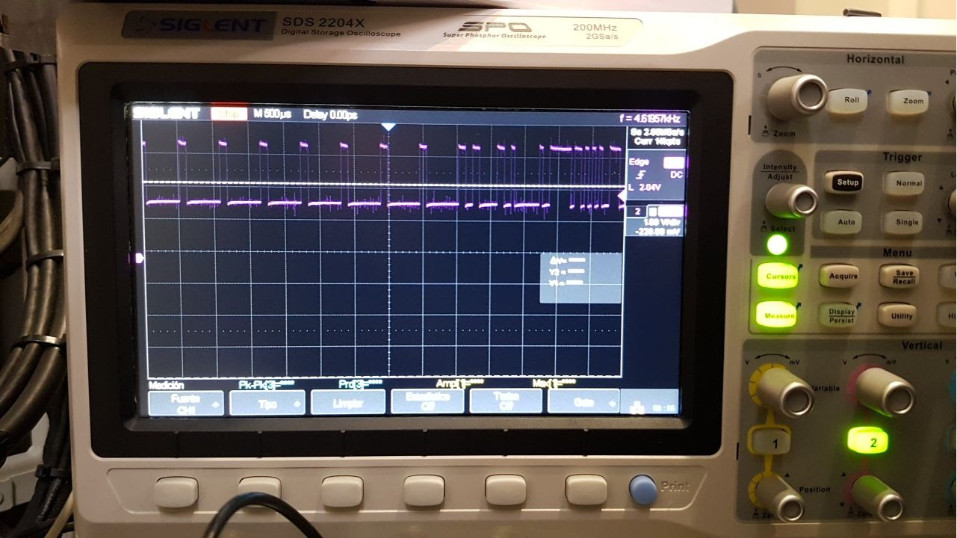
\includegraphics[width=\textwidth]{./Figures/osciloscopio.jpg}
	\caption{Señal MVB capturada en el osciloscopio.}
    \label{fig:osciloscopio}
\end{figure}

Se tomaron varias capturas de un minuto de duración del tráfico del bus MVB, con el banco de medición conectado en diferentes puntos del segmento.
Durante la toma de las capturas se efectuó el procedimiento de encendido de la red y una secuencia de pasos tales como tomar cabina, abrir y cerrar puertas, cambio de marcha, etc., de forma tal de generar tráfico en la red y así poder identificar las variables asociadas a estos eventos.

En la figura~\ref{fig:pulseview} se muestra una visualización de una de las capturas.
En la parte superior se observa que en los primeros 10 ms se transmitieron 10 telegramas, aunque el nivel de detalle no es suficiente para discernir el formato de las tramas.
En la parte inferior se amplía la visualización de uno de los telegramas, donde se puede apreciar en detalle las tramas \textit{master} y \textit{slave}, descriptas en la sección~\ref{sec:tramas}.
Estas visualizaciones se obtuvieron utilizando el software PulseView, que es parte del proyecto Sigrok.

\begin{figure}[htbp!]
	\centering
    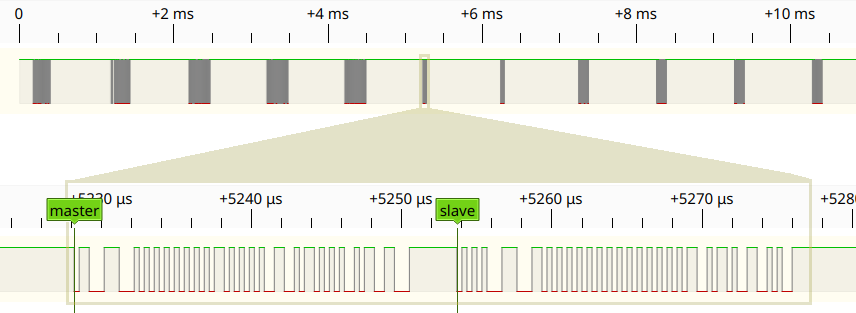
\includegraphics[width=\textwidth]{./Figures/pulseview.png}
    \caption{Visualización de una de las capturas realizadas.}
    \label{fig:pulseview}
\end{figure}

\section{Decodificación de las capturas}
\label{sec:decodificacion}

El siguiente objetivo en la etapa de investigación fue decodificar la información de las tramas capturadas. Para ello se desarrolló un programa en lenguaje Python que toma como entrada una captura en formato binario (un byte por muestra, como se describe en la sección \ref{sec:software}) y produce como salida un reporte de la información decodificada.

El software se compone de dos programas. El primero de ellos, \texttt{mvb\_signal.py}, toma como entrada una captura en formato binario, decodifica los datos codificados en Manchester, y produce como salida un archivo en formato CSV en el que cada línea representa un telegrama y tiene la forma \texttt{<tiempo>,\allowbreak <master>,\allowbreak <slave>}, donde \texttt{<tiempo>} es la marca de tiempo en segundos del telegrama, y \texttt{<master>} y \texttt{<slave>} es el contenido de las tramas en formato hexadecimal, sin incluir los delimitadores y las secuencias de verificación. En el código~\ref{cod:mvbsignal} se muestra un ejemplo de ejecución, en el que se procesa una captura que contiene 4 telegramas.

\begin{lstlisting}[label=cod:mvbsignal,caption=Ejemplo de ejecución de \texttt{mvb\_signal.py}.,float=htbp]
$ python3 mvb_signal.py < captura1.bin
0.0001,4390d6,971e0000008214
0.0011,431bf7,30000f
0.0021,000134,971e07
0.0022,4010c5,04004830580048
\end{lstlisting}

La salida de \texttt{mvb\_signal.py} se puede redireccionar mediante un \textit{pipe} al segundo programa, \texttt{mvbparse.py}, que interpreta la información de las tramas según el protocolo MVB y produce un reporte de la evolución de cada una de las variables identificadas. En el código~\ref{cod:mvbparse} se muestra un ejemplo de ejecución de \texttt{mvbparse.py}.

\begin{lstlisting}[label=cod:mvbparse,caption=Ejemplo de ejecución de \texttt{mvbparse.py}.,float=htbp,basicstyle=\footnotesize\ttfamily]
$ python3 mvb_signal.py < captura2.bin | python3 mvbparse.py
 [[port='0x31b'] [n=   12] [
                  t=  0.001s  0x30000f0c0110000000000000000011a8]],
 [[port='0x353'] [n=    3] [
                  t=  0.212s  0xe2036aa0000000000
                  t=  0.471s  0xe2036ba0000000000
                  t=  0.730s  0xe2036da0000000000]],
\end{lstlisting}

La salida de ejemplo de \texttt{mvbparse.py} indica que se identificaron dos variables, en los puertos \texttt{0x31b} y \texttt{0x353}.
La primera variable fue transmitida en total 12 veces, con un valor de 16 bytes. Se transmitió por primera vez en la marca temporal $0{,}001$ s, con un valor de 16 bytes, y luego se transmitió 11 veces más con el mismo valor.
La variable en el puerto \texttt{0x353} fue transmitida en total 3 veces con un valor de 8 bytes diferente cada vez.

Dado que durante la captura se realizaron diferentes acciones según se mencionó en la sección \ref{sec:capturas} (tomar cabina, abrir y cerrar puertas, etc.), fue posible, analizando la salida producida por el programa, detectar cuáles son las variables que cambian en función del momento en que estas acciones fueron efectuadas. En la figura~\ref{fig:analisis-captura} se muestra, por ejemplo, que la variable en el puerto \texttt{0x1b2} se modifica cada vez que se realizan las acciones de tomar cabina, y seleccionar, abrir y cerrar las puertas.

\begin{figure}[htbp]
	\centering
	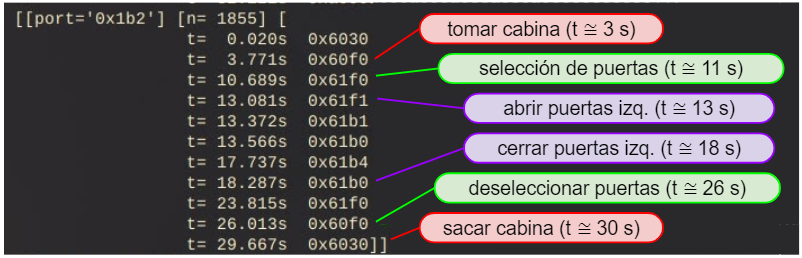
\includegraphics[width=\textwidth]{./Figures/analisis-captura.png}
	\caption[Resultado del análisis de una de las capturas.]{Resultado del análisis de una de las capturas.}
    \label{fig:analisis-captura}
\end{figure}

El software de decodificación está disponible en la plataforma Github \cite{mvbparse-py}. El desarrollo de este prototipo no solo sirvió para proporcionar información valiosa acerca del funcionamiento del bus MVB en las formaciones de Trenes Argentinos, sino también brindó la experiencia necesaria para el posterior desarrollo del software de captura descripto en la sección \ref{sec:software}.

\section{Pruebas del dispositivo de captura}

A continuación se describen los diferentes tipos de pruebas efectuadas para verificar el correcto funcionamiento del dispositivo de captura.

\subsection{Prueba del software de captura}

Para probar el correcto funcionamiento del software de captura (descripto en la sección \ref{sec:software}) se utilizaron las capturas tomadas en la formación ferroviaria (ver sección \ref{sec:capturas}).

Para ejecutar esta prueba se ejecuta el software pasándole como entrada el contenido de una de las capturas en lugar del flujo de datos en tiempo real. Para ello, en una consola se crea un FIFO y se lo alimenta con el contenido de la captura en un ciclo infinito. Se utiliza el comando \texttt{pv} \cite{pv} para limitar el ancho de banda a 12 MB/s:

\begin{lstlisting}
$ mkfifo /tmp/fifo
$ while cat captura.bin; do :; done | pv -L 12M > /tmp/fifo
\end{lstlisting}

En otra consola se ejecuta el software de captura tomando el FIFO como entrada.

\begin{lstlisting}
$ go run cmd/main.go </tmp/fifo
\end{lstlisting}

Esta técnica permite utilizar el software en una PC, como si estuviera conectado al bus MVB.
De esta manera se pudo probar todas sus funcionalidades, tanto en el modo interactivo como en el modo de captura.

\subsection{Prueba de integración de hardware}

% 28 oct 2021?
% 24 nov 2021?

El siguiente paso fue efectuar una prueba de integración del software de captura recibiendo el flujo de datos del VKTECH en tiempo real.
Para ello se utilizó el generador de señal MVB descripto en la sección \ref{sec:generador}, en una configuración como se muestra en la figura~\ref{fig:generador}.
En la figura~\ref{fig:educiaa+vktech} se muestra el banco de medición utilizado en esta prueba.

Esta prueba permitió verificar que es posible utilizar el VKTECH para recibir el flujo de datos en tiempo real.
La prueba se realizó con el software de captura corriendo tanto en una PC como en una Raspberry Pi.

\begin{figure}[htbp]
	\centering
	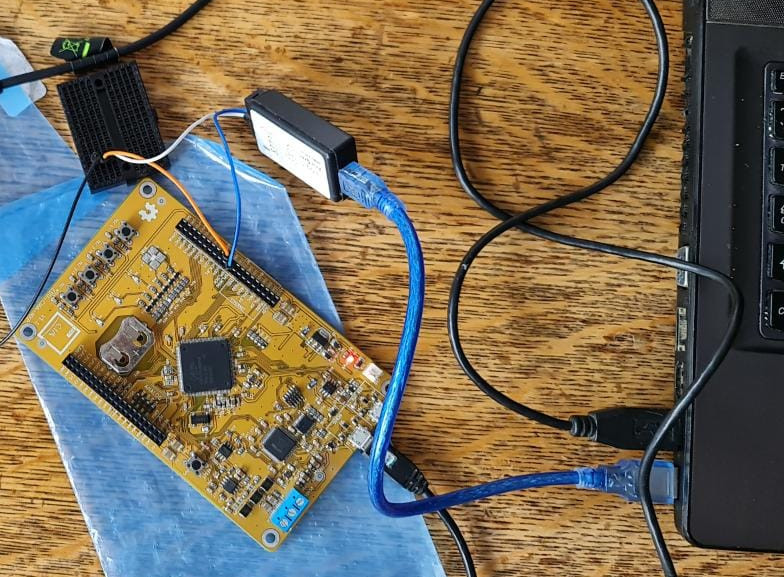
\includegraphics[width=\textwidth]{./Figures/educiaa+vktech.jpg}
	\caption{Banco de medición de la prueba utilizando el generador de señal MVB.}
    \label{fig:educiaa+vktech}
\end{figure}


\subsection{Prueba en una formación ferroviaria}

% 3 dic 2021 (PC)

% 6 ene 2022? (RPI)

La última prueba que se efectuó fue con el dispositivo de captura conectado en el bus MVB en una formación de Trenes Argentinos, como se muestra en la figura~\ref{fig:conexion}.
Se verificó que la conexión del dispositivo de captura no afectó al correcto funcionamiento del resto de los dispositivos conectados en el bus MVB. Cabe destacar que esta prueba se realizó en una formación detenida.

En la figura~\ref{fig:disp-captura-ssh} se muestra una fotografía de la pantalla de la PC utilizada durante la sesión de prueba. En la pantalla se observan dos consolas conectadas a la Raspberry Pi mediante el protocolo SSH. En la consola de la izquierda se ejecuta el comando \texttt{sigrok-cli} para recibir el flujo de datos del VKTECH en tiempo real. En la consola de la derecha se ejecuta el software de captura en modo interactivo.

\begin{figure}[htbp]
	\centering
	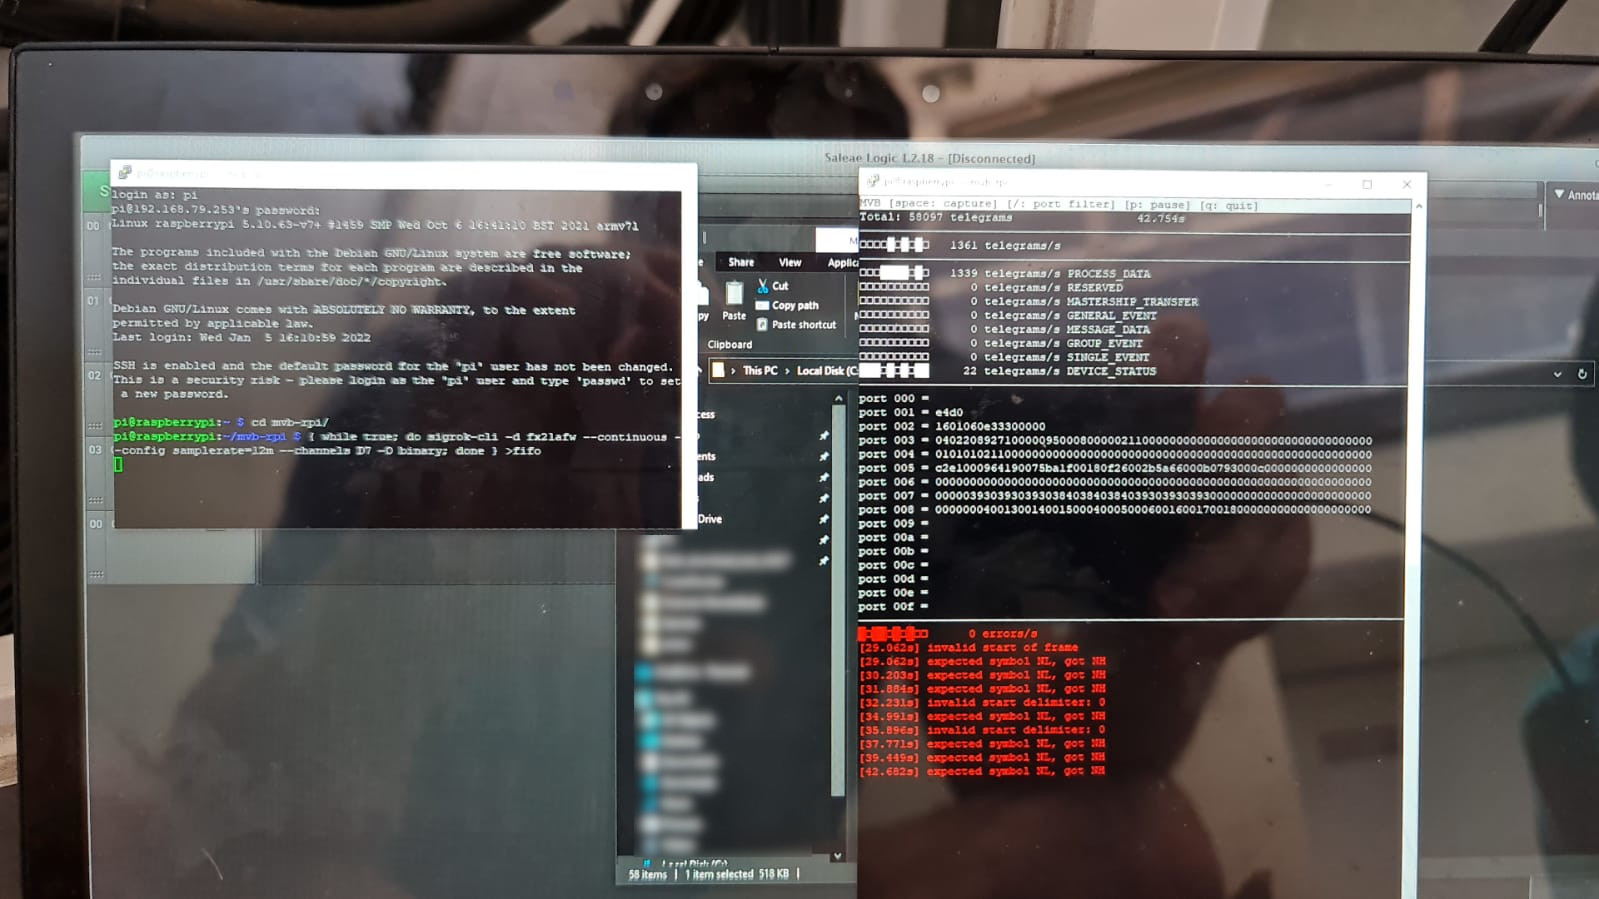
\includegraphics[width=\textwidth]{./Figures/disp-captura-ssh.jpg}
	\caption{Sesión de prueba del dispositivo de captura.}
    \label{fig:disp-captura-ssh}
\end{figure}
 
	% Chapter Template

\chapter{Conclusiones} % Main chapter title

\label{Chapter5} % Change X to a consecutive number; for referencing this chapter elsewhere, use \ref{ChapterX}


%----------------------------------------------------------------------------------------

%----------------------------------------------------------------------------------------
%	SECTION 1
%----------------------------------------------------------------------------------------

\section{Conclusiones generales }

La idea de esta sección es resaltar cuáles son los principales aportes del trabajo realizado y cómo se podría continuar. Debe ser especialmente breve y concisa. Es buena idea usar un listado para enumerar los logros obtenidos.

Algunas preguntas que pueden servir para completar este capítulo:

\begin{itemize}
\item ¿Cuál es el grado de cumplimiento de los requerimientos?
\item ¿Cuán fielmente se puedo seguir la planificación original (cronograma incluido)?
\item ¿Se manifestó algunos de los riesgos identificados en la planificación? ¿Fue efectivo el plan de mitigación? ¿Se debió aplicar alguna otra acción no contemplada previamente?
\item Si se debieron hacer modificaciones a lo planificado ¿Cuáles fueron las causas y los efectos?
\item ¿Qué técnicas resultaron útiles para el desarrollo del proyecto y cuáles no tanto?
\end{itemize}


%----------------------------------------------------------------------------------------
%	SECTION 2
%----------------------------------------------------------------------------------------
\section{Próximos pasos}

Acá se indica cómo se podría continuar el trabajo más adelante.
 
\end{verbatim}

Los apéndices también deben escribirse en archivos .tex separados, que se deben ubicar dentro de la carpeta \emph{Appendices}. Los apéndices vienen comentados por defecto con el caracter \code{\%} y para incluirlos simplemente se debe eliminar dicho caracter.

Finalmente, se encuentra el código para incluir la bibliografía en el documento final.  Este código tampoco debe modificarse. La metodología para trabajar las referencias bibliográficas se desarrolla en la sección \ref{sec:biblio}.
%----------------------------------------------------------------------------------------

\section{Bibliografía}
\label{sec:biblio}

Las opciones de formato de la bibliografía se controlan a través del paquete de latex \option{biblatex} que se incluye en la memoria en el archivo memoria.tex.  Estas opciones determinan cómo se generan las citas bibliográficas en el cuerpo del documento y cómo se genera la bibliografía al final de la memoria.

En el preámbulo se puede encontrar el código que incluye el paquete biblatex, que no requiere ninguna modificación del usuario de la plantilla, y que contiene las siguientes opciones:

\begin{lstlisting}
\usepackage[backend=bibtex,
	natbib=true, 
	style=numeric, 
	sorting=none]
{biblatex}
\end{lstlisting}

En el archivo \file{reference.bib} se encuentran las referencias bibliográficas que se pueden citar en el documento.  Para incorporar una nueva cita al documento lo primero es agregarla en este archivo con todos los campos necesario.  Todas las entradas bibliográficas comienzan con $@$ y una palabra que define el formato de la entrada.  Para cada formato existen campos obligatorios que deben completarse. No importa el orden en que las entradas estén definidas en el archivo .bib.  Tampoco es importante el orden en que estén definidos los campos de una entrada bibliográfica. A continuación se muestran algunos ejemplos:

\begin{lstlisting}
@ARTICLE{ARTICLE:1,
    AUTHOR="John Doe",
    TITLE="Title",
    JOURNAL="Journal",
    YEAR="2017",
}
\end{lstlisting}


\begin{lstlisting}
@BOOK{BOOK:1,
    AUTHOR="John Doe",
    TITLE="The Book without Title",
    PUBLISHER="Dummy Publisher",
    YEAR="2100",
}
\end{lstlisting}


\begin{lstlisting}
@INBOOK{BOOK:2,
    AUTHOR="John Doe",
    TITLE="The Book without Title",
    PUBLISHER="Dummy Publisher",
    YEAR="2100",
    PAGES="100-200",
}
\end{lstlisting}


\begin{lstlisting}
@MISC{WEBSITE:1,
    HOWPUBLISHED = "\url{http://example.com}",
    AUTHOR = "Intel",
    TITLE = "Example Website",
    MONTH = "12",
    YEAR = "1988",
    URLDATE = {2012-11-26}
}
\end{lstlisting}

Se debe notar que los nombres \emph{ARTICLE:1}, \emph{BOOK:1}, \emph{BOOK:2} y \emph{WEBSITE:1} son nombres de fantasía que le sirve al autor del documento para identificar la entrada. En este sentido, se podrían reemplazar por cualquier otro nombre.  Tampoco es necesario poner : seguido de un número, en los ejemplos sólo se incluye como un posible estilo para identificar las entradas.

La entradas se citan en el documento con el comando: 

\begin{verbatim}
\citep{nombre_de_la_entrada}
\end{verbatim}

Y cuando se usan, se muestran así: \citep{ARTICLE:1}, \citep{BOOK:1}, \citep{BOOK:2}, \citep{WEBSITE:1}.  Notar cómo se conforma la sección Bibliografía al final del documento. 

\chapter{Introducción específica}

En este capítulo se presenta un resumen de los conceptos más relevantes acerca de la red TCN y su implementación en las formaciones de Trenes Argentinos, y se detallan las diferentes tecnologías utilizadas para el desarrollo del dispositivo de captura.

\section{La red TCN}

La red TCN es una combinación jerárquica de dos buses de datos en los que se transmite información dentro de una formación ferroviaria. El \textit{Multifunction Vehicle Bus} (MVB) interconecta los diferentes dispositivos presentes dentro de cada vehículo, y el \textit{Wire Train Bus} (WTB) interconecta los diferentes vehículos. Los componentes de la red TCN están estandarizados en la norma IEC 61375-1. En la figura~\ref{fig:tcn-mvb-wtb} se muestra un diagrama simplificado de la arquitectura TCN.

\begin{figure}[htbp]
	\centering
    {
        \fontfamily{phv}
        \fontsize{9pt}{9pt}\selectfont
        \input{./Figures/tcn-mvb-wtb.pdf_tex}
    }
	\caption[\textit{Wire Train Bus} y \textit{Multifunction Vehicle Bus}]{\textit{Wire Train Bus} y \textit{Multifunction Vehicle Bus}.\footnotemark}
    \label{fig:tcn-mvb-wtb}
\end{figure}
\footnotetext{Dibujo del tren por Freepik\\(\url{https://www.freepik.com/free-vector/collection-different-types-trains_1114167.htm})}

Dado que el dispositivo desarrollado se conecta al bus MVB, a continuación se exponen las características principales de este bus de comunicación.

\subsection{El bus MVB}

El bus MVB interconecta diferentes dispositivos ubicados en el mismo vehículo o en diferentes vehículos que no son separados con frecuencia. El MVB puede direccionar hasta 4095 dispositivos de distintos tipos, desde simples sensores y actuadores hasta equipos programables.

La estructura de MVB sigue el modelo OSI \cite{ISO7498-1}, que establece siete capas de abstracción en el proceso de transmisión de datos.
En las capas inferiores del protocolo MVB se establecen las características del medio físico y la estructura de las tramas y telegramas.
A continuación, se describen estos conceptos, que son los más relevantes para el desarrollo de este trabajo.

\subsection{Capa física}

El bus MVB ofrece tres opciones de medios físicos para la capa inferior:

\begin{itemize}
\item El medio \textit{Electrical Short Distance} (ESD), para distancias de hasta 20~m, que soporta hasta 32 dispositivos por segmento, con transceptores de tipo RS-485.
\item El medio \textit{Electrical Middle Distance} (EMD), para distancias de hasta 200~m, que soporta hasta  32 dispositivos por segmento, con transformadores y transceptores compatibles con la norma IEC 61158-2 \cite{iec61158_2}.
\item El medio \textit{Optical Glass Fibre} (OGF), para distancias de hasta 2000~m, y soporta conexiones punto a punto o subredes de topología tipo estrella.
\end{itemize}

Puede haber diferentes buses en un vehículo, interconectados mediante un \textit{gateway} al bus WTB.
También es posible que el bus MVB abarque más de un vehículo, y en este caso la norma recomienda el medio EMD.
Un ejemplo de esta configuración se ilustra en la figura~\ref{fig:emd-esd-wtb}.

\begin{figure}[htbp]
	\centering
    {
        \fontfamily{phv}
        \fontsize{9pt}{9pt}\selectfont
        \input{./Figures/medios.pdf_tex}
    }
	\caption[MVB abarcando tres vehículos]{MVB abarcando tres vehículos.}
    \label{fig:emd-esd-wtb}
\end{figure}

En la figura~\ref{fig:segmento} se ilustra un segmento EMD.
Cada dispositivo conectado a un segmento EMD tiene dos conectores D-sub de 9 pines (DE-9) que van, respectivamente, al dispositivo anterior y siguiente en el segmento. Los dispositivos en los extremos del segmento tienen un terminador.

\begin{figure}[htbp]
	\centering
    {
        \fontfamily{phv}
        \fontsize{9pt}{9pt}\selectfont
        \input{./Figures/segmento-emd.pdf_tex}
    }
	\caption[Un segmento EMD]{Un segmento EMD.}
    \label{fig:segmento}
\end{figure}

En la figura~\ref{fig:pines} se muestra la configuración de pines de los conectores.
La transmisión de la señal digital se realiza mediante la tensión diferencial entre los pares Data\_N y Data\_P. La norma permite que haya una única línea (A) o dos líneas (A y B) para proporcionar redundancia.

\begin{figure}[htbp]
	\centering
    {
        \fontfamily{phv}
        \fontsize{8pt}{8pt}\selectfont
        \input{./Figures/db9-emd.pdf_tex}
    }
	\caption[Configuración de pines del conector D-sub de 9 pines del medio EMD]{Configuración de pines del conector DE-9 del medio EMD. Se omite por simplicidad la interconexión de los pines 6 a 9, que se utilizan para los terminadores.}
    \label{fig:pines}
\end{figure}

\subsection{Tramas}
\label{sec:tramas}

Se denomina ``trama'' a un paquete de datos transmitido por un dispositivo.
En el bus MVB se transmiten dos tipos de tramas:

\begin{itemize}
\item La trama \textit{master}, que es transmitida únicamente por el dispositivo maestro del bus.
\item La trama \textit{slave}, que es transmitida por un dispositivo esclavo en respuesta a una trama \textit{master}.
\end{itemize}

Todos los medios MVB operan a una velocidad unificada de 1,5~Mbit/s.
La información se transmite utilizando una codificación Manchester, que combina en una única señal la información y el \textit{clock}.

La transmisión de una trama se compone de un delimitador inicial (SD) de 9 bits de duración, los datos de la trama, una secuencia de verificación (CS) de 8 bits y un delimitador final (ED) de 2 bits de duración.
En los datos de la trama y la secuencia de verificación, un ``1'' se transmite como una transición negativa en el medio de una celda de bit, y un ``0'' se transmite como una transición positiva.
Los delimitadores de inicio para las tramas \textit{master} y \textit{slave} son diferentes, y se denominan MSD y SSD.
En la figura~\ref{fig:manchester} se muestra a modo de ejemplo la transmisión de una trama \textit{master} en el medio EMD.

\begin{figure}[htbp]
	\centering
    {
        \fontfamily{phv}
        \fontsize{8pt}{8pt}\selectfont
        \input{./Figures/manchester.pdf_tex}
    }
	\caption[Transmisión de una trama master]{Transmisión de una trama \textit{master}.}
    \label{fig:manchester}
\end{figure}


\subsection{Telegramas}

Una secuencia de una trama \textit{master} seguida de una trama \textit{slave} conforman un telegrama, como se muestra en la figura~\ref{fig:telegrama}.

\begin{figure}[htbp]
	\centering
    {
        \fontfamily{phv}
        \fontsize{8pt}{8pt}\selectfont
        \input{./Figures/telegrama.pdf_tex}
    }
	\caption[Un telegrama MVB]{Un telegrama MVB.}
    \label{fig:telegrama}
\end{figure}

Las tramas \textit{master} tienen una longitud fija de 16 bits (sin contar los delimitadores), e incluyen:

\begin{itemize}
\item Un código de 4 bits llamado \texttt{F\_code}, que indica el tipo y tamaño de la trama \textit{slave} esperada a continuación.
\item Un campo de 12 bits, que puede contener una dirección de destino, o parámetros específicos al \texttt{F\_code}.
\end{itemize}

Todos los dispositivos conectados al bus decodifican la trama \textit{master}. El dispositivo encuestado luego responde con su trama \textit{slave}, que a su vez puede ser recibida por otros dispositivos.

\subsection{Variables}

Son de particular interés los telegramas con \texttt{F\_code} entre 0 y 4, que se denominan \texttt{Process\_Data}.
En este caso, el campo de 12 bits contiene una dirección lógica que hace referencia a un puerto.
Cada puerto está asociado unívocamente a una variable, que puede contener uno o más valores como la velocidad actual, la tensión de red, el estado de las puertas, etc.
Cada dispositivo \textit{slave} almacena uno o más puertos, y al ser encuestado responde con el valor actual de la variable correspondiente.

\section{Red TCN en las formaciones de Trenes Argentinos}

En la figura~\ref{fig:tms} se muestra un diagrama simplificado de la topología de la red TCN en una sección de 3 vehículos EMU de una formación de Trenes Argentinos. En el diagrama se observa que los buses MVB están implementados con el medio físico EMD.

\begin{figure}[htbp]
	\centering
    {
        \fontfamily{phv}
        \fontsize{8pt}{8pt}\selectfont
        \input{./Figures/tms.pdf_tex}
    }
	\caption[Topología de la red TCN en una formación de Trenes Argentinos]{Topología de la red TCN en una formación de Trenes Argentinos.}
    \label{fig:tms}
\end{figure}

\pagebreak

En la figura~\ref{fig:rcme} se muestra una fotografía de uno de los dispositivos presentes en la cabina del conductor de una formación de la línea Mitre. Se trata del módulo de comunicación RCMe, que controla las puertas, el sistema de aire acondicionado y el sistema de información al pasajero. En el panel frontal del módulo RCMe, los conectores DE-9 X1 y X2 (destacados en la figura) corresponden al bus MVB.

\begin{figure}[htbp]
	\centering
	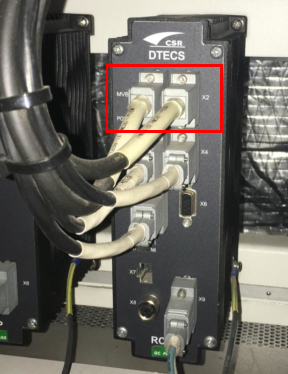
\includegraphics[width=0.5\textwidth]{./Figures/RCMe.pdf}
	\caption[El módulo de comunicación RCMe]{El módulo de comunicación RCMe presente en un EMU. Los dos conectores DE-9 destacados corresponden al bus MVB.}
    \label{fig:rcme}
\end{figure}

La pantalla HMI (\textit{Human Machine Interface}), también ubicada en la cabina del conductor, tiene un modo de operación que permite visualizar el valor de algunas variables que son transmitidas periódicamente en forma de \texttt{Process\_Data}. En la figura~\ref{fig:hmi} se puede observar que en el puerto 0 hay una variable de 16 bits cuyo valor binario actual es 1100 0001 0110 0101, o 33702 si se interpreta como un número decimal.

\begin{figure}[htbp]
	\centering
	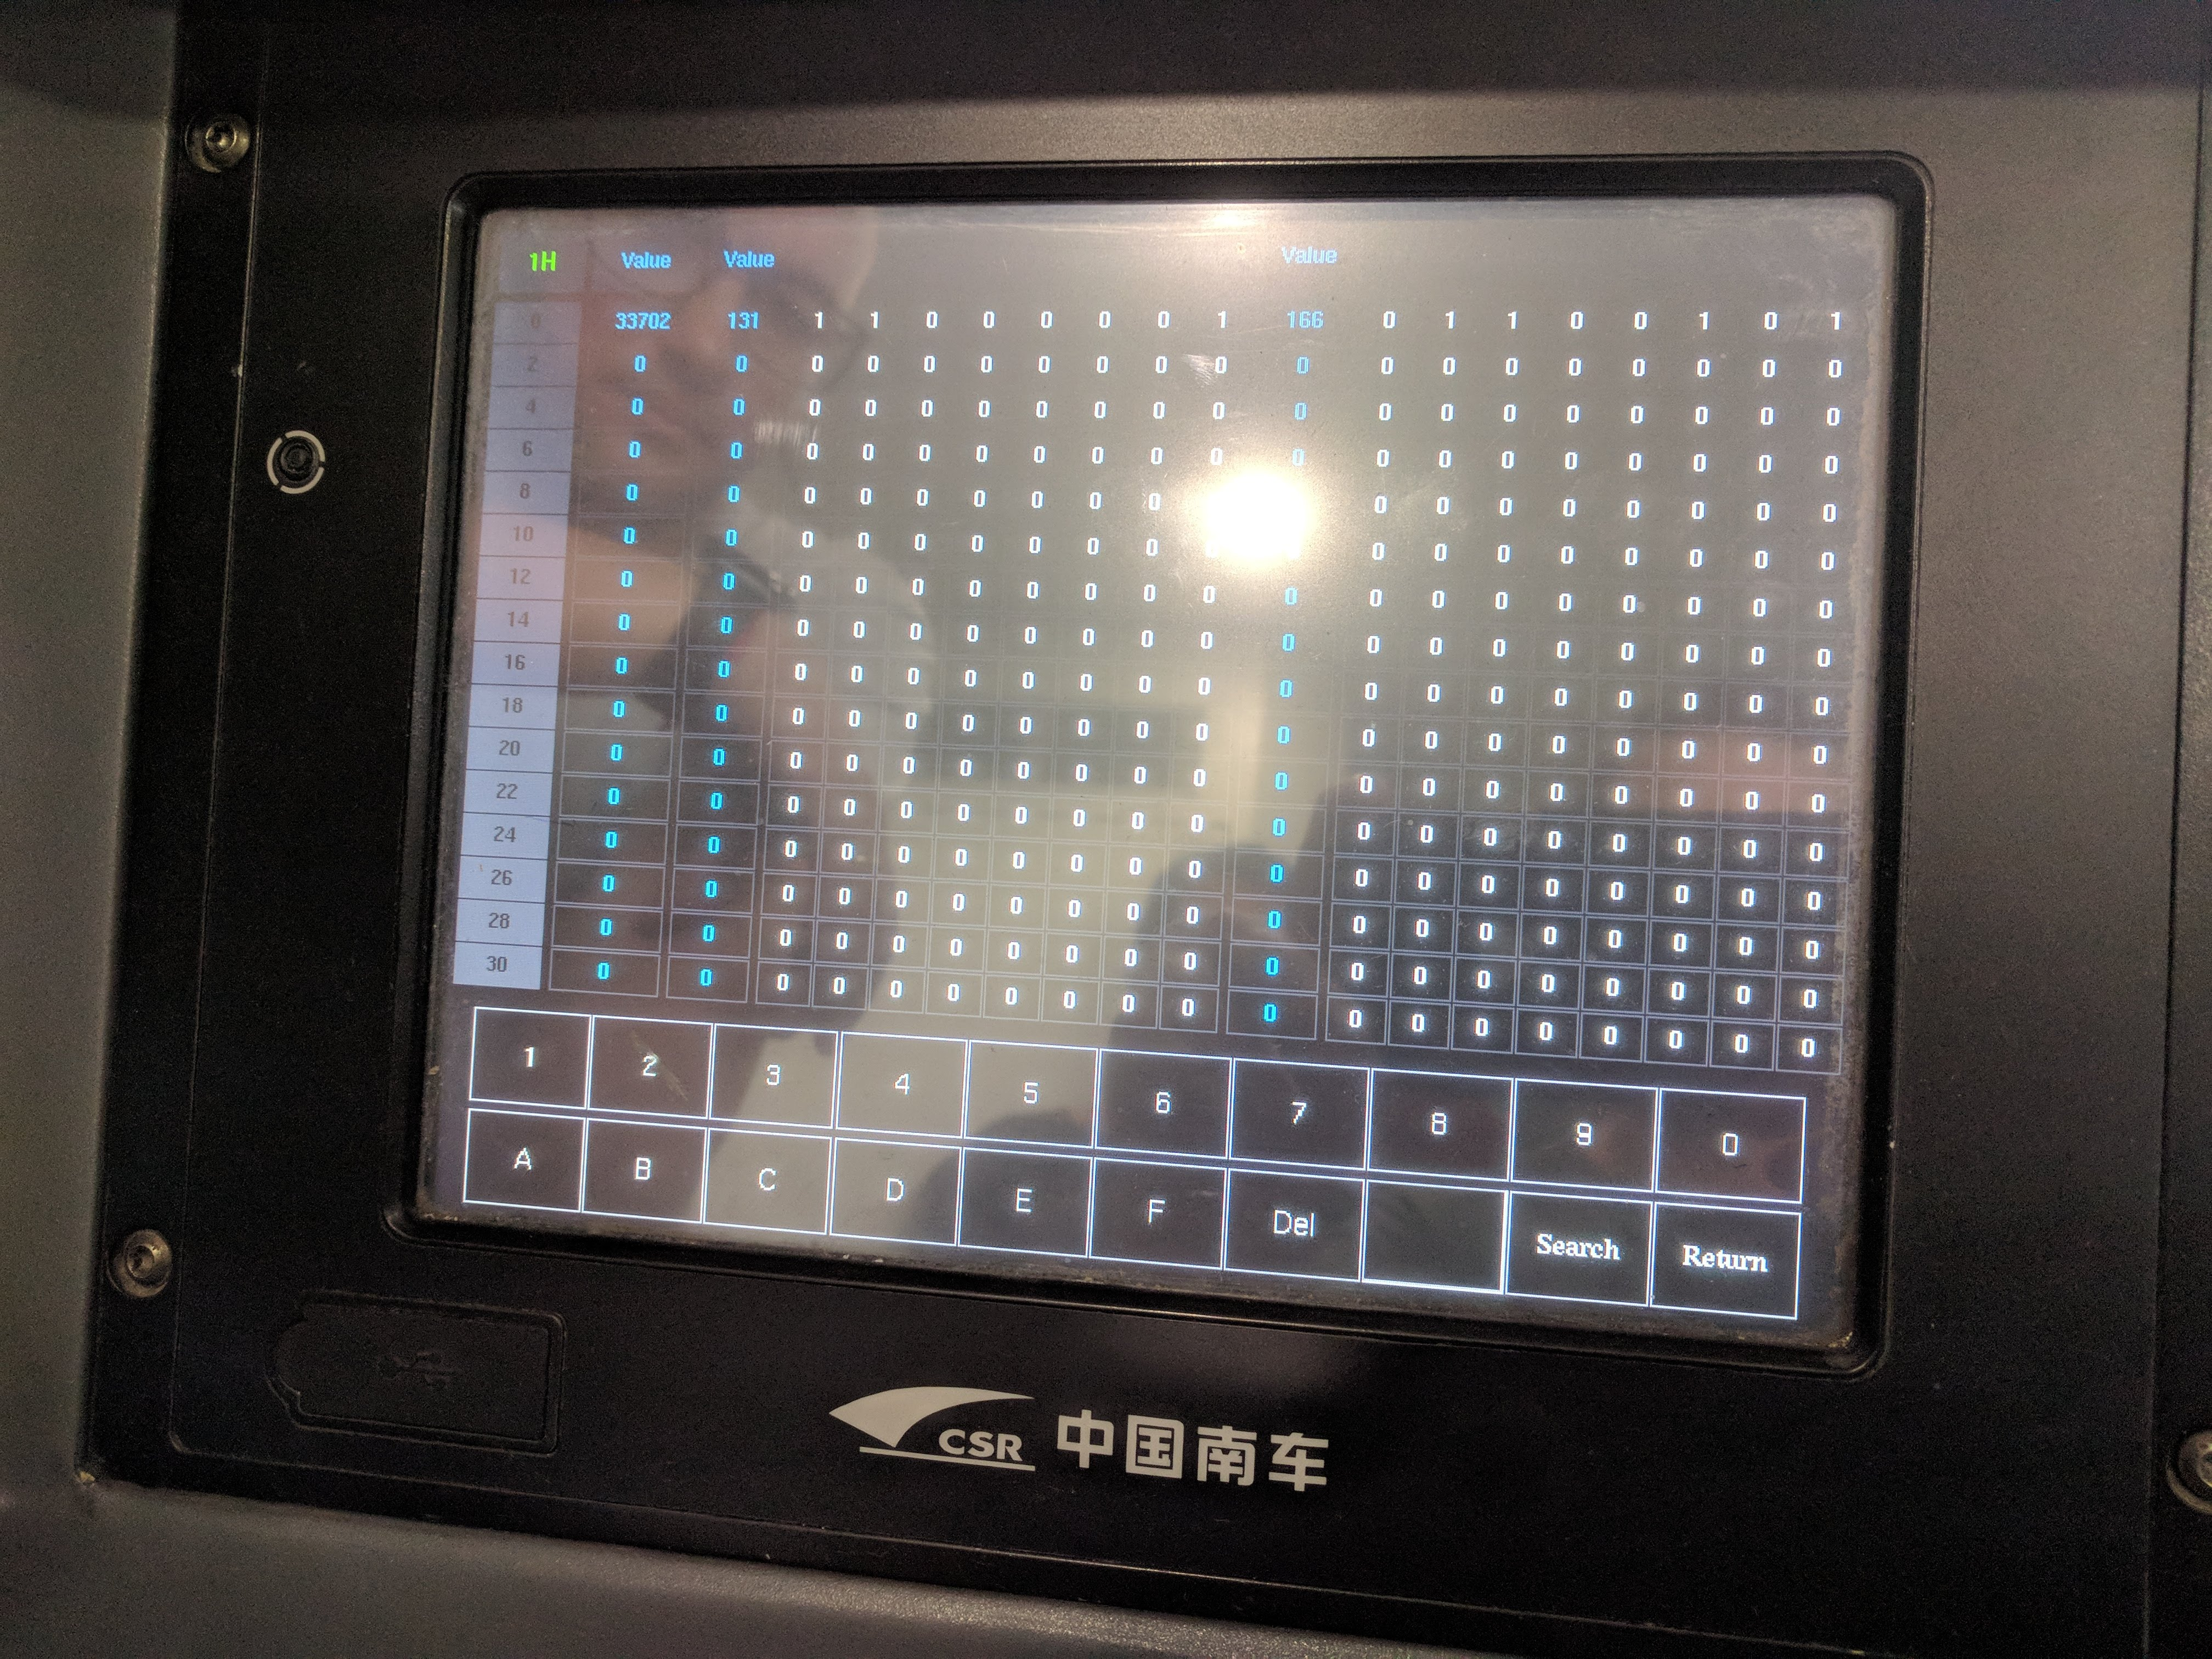
\includegraphics[width=1\textwidth]{./Figures/hmi.jpg}
	\caption[El HMI mostrando algunas variables]{El HMI mostrando algunas variables.}
    \label{fig:hmi}
\end{figure}

\section{Componentes del sistema}

A continuación, se describen las principales tecnologías utilizadas para el desarrollo del dispositivo de captura.

\subsection{EDU-CIAA}

La EDU-CIAA \cite{web:ciaa} es una plataforma de desarrollo de hardware libre basada en el microcontrolador NXP LPC4337 \cite{web:lpc4337} (dual core ARM Cortex-M4F y Cortex-M0), diseñada para la enseñanza de la programación y el desarrollo de sistemas embebidos en Argentina y otros países de habla hispana.
Esta placa cuenta con múltiples interfaces de entrada/salida, como puertos USB, Ethernet, CAN, UART, I²C, SPI, ADC y DAC.

La EDU-CIAA se utilizó para desarrollar un generador de señal MVB que permitió probar el funcionamiento del dispositivo de captura sin necesidad de conectarlo en una formación ferroviaria. El diseño del generador se describe en la sección \ref{sec:generador}.

\subsection{Raspberry Pi}

La Raspberry Pi \cite{web:rpi} es una computadora de placa única (SBC, por sus siglas en inglés) de bajo costo y tamaño reducido, diseñada por la \textit{Raspberry Pi Foundation} para promover la enseñanza de la informática básica en las escuelas y países en desarrollo.
Entre sus capacidades se encuentran el procesamiento de video en alta definición, conectividad inalámbrica y soporte para una gran cantidad de periféricos, lo que la convierte en una opción popular para una amplia gama de proyectos, desde la automatización del hogar hasta la robótica y la creación de servidores web.

El dispositivo de captura desarrollado en este trabajo está basado en la Raspberry Pi. Su diseño se describe en la sección \ref{sec:hardware}.

\subsection{Analizador lógico VKTECH y Sigrok}

El analizador lógico VKTECH \cite{vktech} es un dispositivo que permite capturar y analizar señales digitales en sistemas electrónicos. El dispositivo provee 8 canales que pueden capturar con una frecuencia de muestreo de hasta 24MHz, y cuenta con una interfaz USB 2.0 para conectar a una PC.

Sigrok \cite{sigrok} es un software libre y de código abierto que proporciona una plataforma para la adquisición y análisis de datos de múltiples tipos de instrumentos de medición, incluyendo analizadores lógicos, osciloscopios y multímetros. La herramienta es compatible con una amplia gama de dispositivos y marcas, lo que permite la integración de diferentes equipos y protocolos de comunicación en un solo entorno de software. Además, Sigrok ofrece una interfaz gráfica intuitiva y fácil de usar, así como una API para el desarrollo de aplicaciones personalizadas.

En este trabajo se utilizó el analizador lógico VKTECH y Sigrok en la fase de investigación, para realizar capturas del tráfico del bus MVB y analizarlas, como se menciona en las secciones \ref{sec:capturas} y \ref{sec:decodificacion}.

El dispositivo de captura desarrollado también utiliza el analizador lógico VKTECH y Sigrok para capturar el tráfico del bus en tiempo real, como se describe en las secciones \ref{sec:hardware} y  \ref{sec:software}.

\subsection{Python}

Python \cite{web:python} es un lenguaje de programación interpretado, de alto nivel y de propósito general. Está diseñado para ser fácil de aprender y cuenta con una sintaxis clara y legible.
Además tiene una amplia variedad de librerías y frameworks disponibles que permiten desarrollar aplicaciones en diferentes áreas, como ciencia de datos, inteligencia artificial, automatización y desarrollo web.

En este trabajo se utilizó el lenguaje Python en la fase de investigación, para decodificar las primeras capturas realizadas en la formación, como se describe en la sección \ref{sec:capturas}.

\subsection{Go}

Go \cite{web:go} es un lenguaje de programación de código abierto desarrollado por Google.
Se trata de un lenguaje de alto nivel, compilado, con tipos estáticos y recolector de basura.
Es sintácticamente similar al lenguaje C, pero se caracteriza por su enfoque en la concurrencia, la eficiencia y la simplicidad en la escritura de código.

Se utilizó el lenguaje Go para escribir el software del dispositivo de captura que corre en la Raspberry Pi, como se describe en la sección \ref{sec:software}.
 
\chapter{Diseño e implementación}
\label{cap:DisenioImplementacion}

En este capítulo se presenta la arquitectura de hardware y software del dispositivo de captura, como así también del generador de señal MVB desarrollado para probar el dispositivo de captura sin necesidad de conectarlo en una formación ferroviaria.

\section{Arquitectura de hardware}
\label{sec:hardware}

Como se muestra en la figura~\ref{fig:conexion}, el dispositivo de captura tiene dos conectores DE-9 compatibles con el medio EMD. De esta manera se lo puede conectar a un segmento MVB entre dos dispositivos cualesquiera.

\begin{figure}[htbp]
	\centering
    {
        \fontfamily{phv}
        \fontsize{8pt}{8pt}\selectfont
        \input{./Figures/conexion.pdf_tex}
    }
	\caption{Conexión del dispositivo de captura en un segmento EMD.}
    \label{fig:conexion}
\end{figure}

En la figura~\ref{fig:bloques} se muestra un diagrama de la arquitectura del dispositivo de captura.
Se dejan en corto circuito las líneas de transmisión (ver figura~\ref{fig:pines}), de forma tal de que el dispositivo opere en forma pasiva. Salvando la impedancia que agrega a la línea, el dispositivo de captura es transparente para el resto de los dispositivos del segmento.
El dispositivo MAX485 \cite{max485} se utiliza para convertir la señal de entrada (par diferencial $-$5~V - +5~V) a una señal compatible para el analizador lógico VKTECH (0~V - +5~V). El analizador lógico se conecta a una Raspberry Pi mediante un puerto USB 2.0. La Raspberry Pi decodifica las tramas por software y almacena los datos capturados en una tarjeta de memoria. Mediante su interfaz Wi-Fi se puede conectar una PC (utilizando el protocolo SSH) para descargar las capturas, y también para visualizar el tráfico del bus MVB en tiempo real.

\begin{figure}[htbp]
	\centering
    {
        \fontfamily{phv}
        \fontsize{8pt}{8pt}\selectfont
        \input{./Figures/bloques.pdf_tex}
    }
	\caption{Arquitectura de hardware del dispositivo de captura.}
    \label{fig:bloques}
\end{figure}

En la figura~\ref{fig:esquematico} se muestra un diagrama esquemático con el detalle de las conexiones entre los diferentes componentes. En el diagrama se utiliza la etiqueta ``USB'' para representar la conexión a la Raspberry Pi, que no se muestra por simplicidad. Asimismo, la conexión ``VCC'' del MAX485 se conecta al pin número 2 del conector GPIO de la Raspberry Pi \cite{gpio}.

\begin{figure}[htbp]
	\centering
	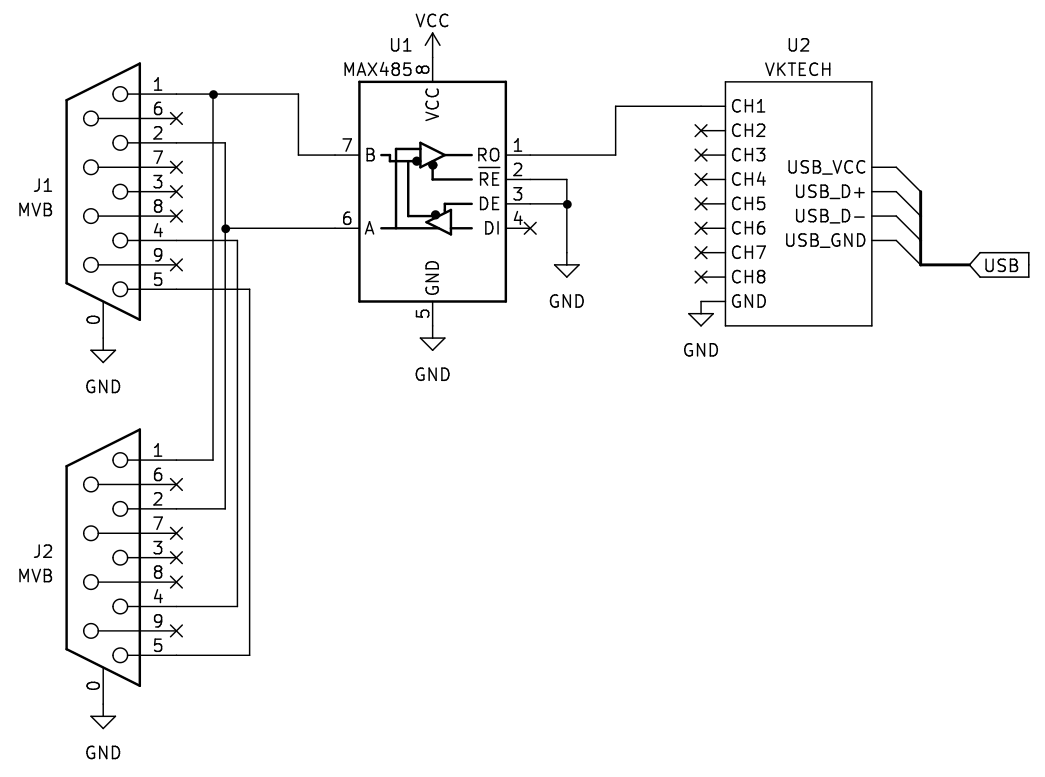
\includegraphics[width=1\textwidth]{./Figures/esquematico.png}
	\caption{Diagrama esquemático del dispositivo de captura.}
    \label{fig:esquematico}
\end{figure}

En la figura~\ref{fig:fotodispositivo} se muestra una foto del dispositivo de captura en construcción. Cabe aclarar que en el dispositivo hay cuatro MAX485 para permitir, en el futuro, capturar ambas líneas A y B del segmento EMD, o bien capturar dos o más segmentos diferentes. En esta primera versión del dispositivo se utiliza solo uno de los MAX485.

\begin{figure}[htbp]
	\centering
	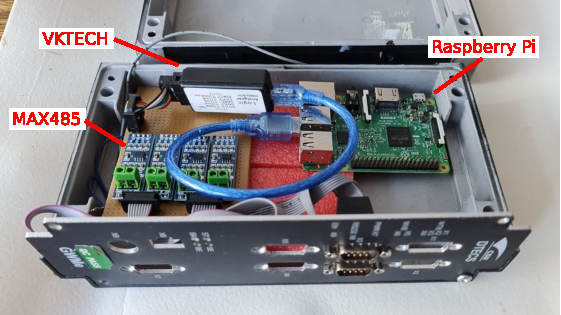
\includegraphics[width=1\textwidth]{./Figures/foto-dispositivo.pdf}
	\caption{Foto del dispositivo de captura en construcción.}
    \label{fig:fotodispositivo}
\end{figure}

\section{Arquitectura de software}
\label{sec:software}

Como se ve en la figura~\ref{fig:bloques}, a la Raspberry Pi entra la señal digital capturada por el analizador lógico en tiempo real, mediante la interfaz USB. Para recibir esta señal se utiliza Sigrok, invocándolo de la siguiente manera:

\begin{lstlisting}
sigrok-cli -d fx2lafw --continuous --config samplerate=12m
           --channels D0 -O binary
\end{lstlisting}

Este comando recibe la señal del VKTECH en la interfaz USB, muestrea la señal digital con una frecuencia de 12 MHz y produce como salida un flujo de datos que se puede redireccionar a un archivo o a un \textit{pipe} de Unix.
Por cada muestra capturada, se emite un byte en el que el bit menos significativo es 0 o 1 dependiendo de si la señal lógica capturada es baja o alta.
De esta forma, el flujo de datos tiene un ancho de banda de 12 MB/s, aunque solo se usa uno de los 8 bits de cada byte.
En la figura~\ref{fig:sigrok} se muestra un ejemplo del flujo de datos producido por Sigrok.

\begin{figure}[htbp]
	\centering
    {
        \fontfamily{phv}
        \fontsize{9pt}{9pt}\selectfont
        \input{./Figures/sigrok.pdf_tex}
    }
	\caption{Flujo de datos producido por Sigrok.}
    \label{fig:sigrok}
\end{figure}

Sería posible bajar la frecuencia de captura a 6 MHz, pero no menos ya que el protocolo MVB transmite la señal a 1,5 Mbit/s en codificación Manchester.
Para lograr una captura suficientemente confiable se necesita que la frecuencia de muestreo sea de al menos 6 MHz.
La frecuencia elegida de 12 MHz ofrece un buen balance entre confiabilidad y eficiencia en espacio.

\pagebreak

El flujo de datos producido por Sigrok se redirecciona mediante un \textit{pipe} de Unix a un software programado en lenguaje Go. Como se muestra en la figura~\ref{fig:capas-software}, la decodificación se realiza en tres capas de procesamiento:

\begin{enumerate}
\item La capa inferior (\texttt{MVBStream}) lee el flujo de datos byte por byte y ofrece funcionalidades tales como leer muestras individualmente, esperar hasta la siguiente transición de estado (alto-bajo o bajo-alto), esperar una cantidad de tiempo, etc.
\item La capa intermedia (\texttt{MVBDecoder}) identifica las tramas MVB y por cada telegrama produce un evento (\texttt{Event}).
\item La capa superior recibe los eventos y los procesa según el modo de operación del software. Se ofrecen dos modos de operación:
    \begin{itemize}
        \item En el modo interactivo, el software presenta una interfaz de usuario en la que se muestra el tráfico MVB en tiempo real. En la figura~\ref{fig:interactivo} se muestra una captura de pantalla del modo interactivo.
        \item En el modo de almacenamiento, el software permite almacenar la evolución histórica de una o más variables de importancia.
    \end{itemize}
\end{enumerate}

\begin{figure}[htbp]
	\centering
    {
        \fontfamily{phv}
        \fontsize{9pt}{9pt}\selectfont
        \input{./Figures/capas-software.pdf_tex}
    }
	\caption{Capas de procesamiento del software de captura.}
    \label{fig:capas-software}
\end{figure}

\begin{figure}[htbp]
	\centering
	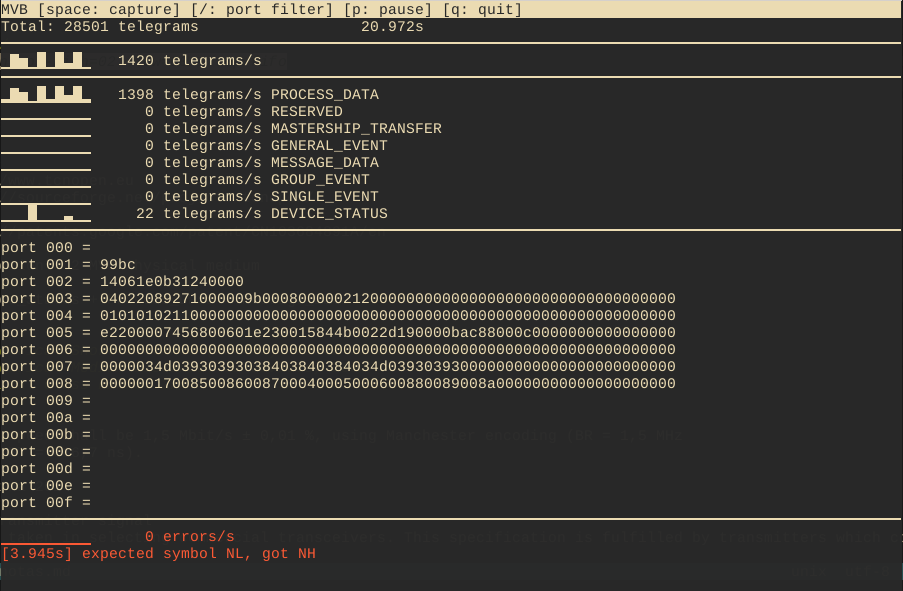
\includegraphics[width=1\textwidth]{./Figures/modo-interactivo.png}
	\caption{Modo interactivo del software de captura.}
    \label{fig:interactivo}
\end{figure}

El código fuente de este programa está disponible en la plataforma Github \cite{mvbparse-go}.
En el archivo \texttt{README.md} se muestran más detalles acerca de los diferentes modos de funcionamiento.

\section{Dispositivo generador de señal}
\label{sec:generador}

\chapter{Ensayos y resultados}

\label{cap:EnsayosResultados}

En este capítulo se describe la fase de investigación previa al desarrollo del dispositivo de captura, junto con las pruebas realizadas para validar su correcto funcionamiento, tanto en un entorno de laboratorio como en una formación de Trenes Argentinos.

\section{Capturas del tráfico de la red en una formación}
\label{sec:capturas}

Como parte de la etapa de investigación, se realizaron visitas a los talleres de Trenes Argentinos en Victoria y Castelar, coordinadas respectivamente por Sergio Dieleke (Laboratorio Electrónico, Subgerencia de Material Rodante Línea Mitre) y Bruno Pilato (Laboratorio de Electrónica de Castelar, Línea Sarmiento).
El objetivo principal de estas visitas fue tomar capturas del tráfico del bus MVB, para ganar conocimiento acerca del estándar TCN y de la implementación particular en las EMU de Trenes Argentinos.

Para tomar las capturas se conectó un MAX485 y un analizador lógico VKTECH entre dos dispositivos MVB.
Se utilizó una PC para controlar el VKTECH y almacenar las diferentes capturas.
También se utilizó un osciloscopio para verificar que la señal capturada tuviera las características esperadas.
En la figura~\ref{fig:banco-capturas} se muestra un diagrama de bloques del banco de medición.
En las figuras~\ref{fig:foto-banco-capturas} y \ref{fig:osciloscopio} se muestra una fotografía del banco de medición y un detalle de la señal capturada en el osciloscopio.

% video con la secuencia https://drive.google.com/drive/folders/1I-V33ElLX13Iy0YliUeojRwYFQKuucAO
\begin{figure}[htbp]
	\centering
    {
        \fontfamily{phv}
        \fontsize{9pt}{9pt}\selectfont
        \input{./Figures/banco-captura.pdf_tex}
    }
	\caption{Banco de medición utilizado para tomar las capturas.}
    \label{fig:banco-capturas}
\end{figure}

\begin{figure}[htbp]
	\centering
	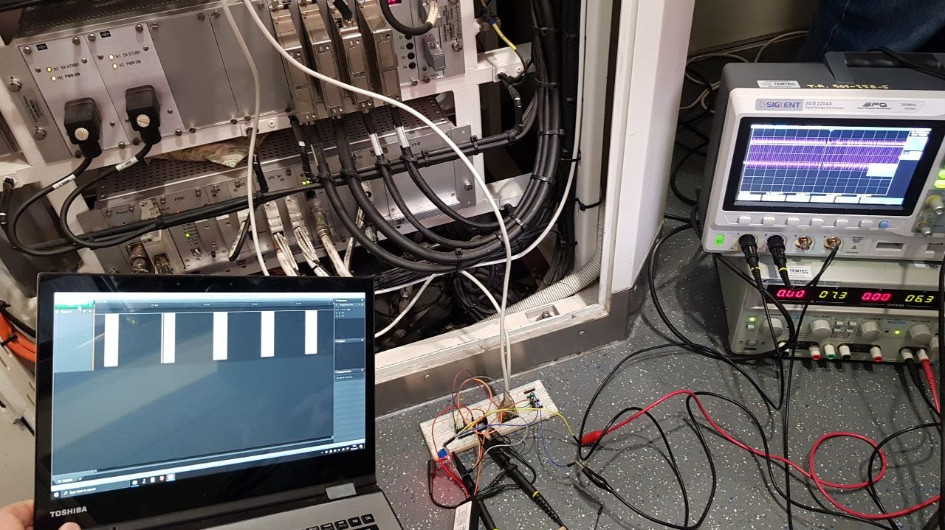
\includegraphics[width=\textwidth]{./Figures/foto-capturas.jpg}
	\caption{Fotografía del banco de medición utilizado para tomar las capturas.}
    \label{fig:foto-banco-capturas}
\end{figure}

\begin{figure}[htbp]
	\centering
	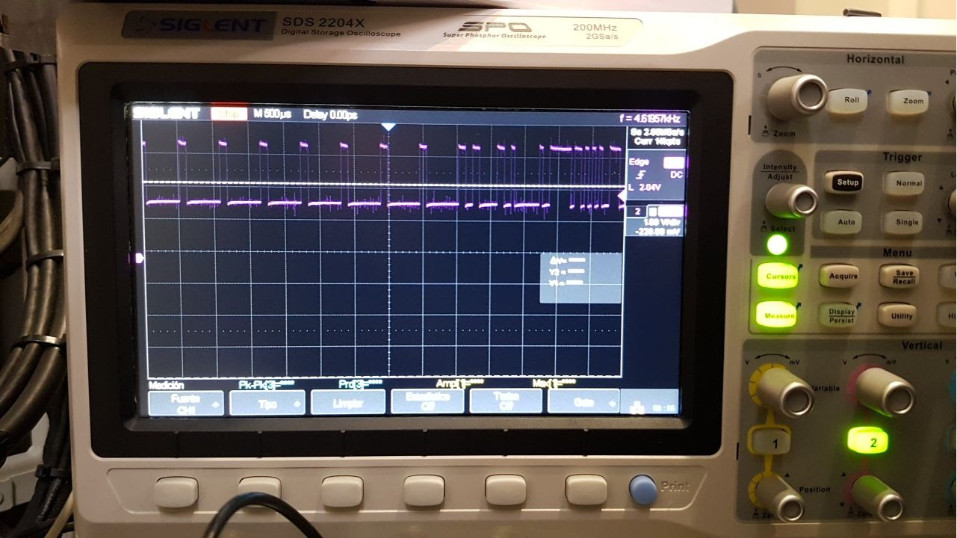
\includegraphics[width=\textwidth]{./Figures/osciloscopio.jpg}
	\caption{Señal MVB capturada en el osciloscopio.}
    \label{fig:osciloscopio}
\end{figure}

Se tomaron varias capturas de un minuto de duración del tráfico del bus MVB, con el banco de medición conectado en diferentes puntos del segmento.
Durante la toma de las capturas se efectuó el procedimiento de encendido de la red y una secuencia de pasos tales como tomar cabina, abrir y cerrar puertas, cambio de marcha, etc., de forma tal de generar tráfico en la red y así poder identificar las variables asociadas a estos eventos.

En la figura~\ref{fig:pulseview} se muestra una visualización de una de las capturas.
En la parte superior se observa que en los primeros 10 ms se transmitieron 10 telegramas, aunque el nivel de detalle no es suficiente para discernir el formato de las tramas.
En la parte inferior se amplía la visualización de uno de los telegramas, donde se puede apreciar en detalle las tramas \textit{master} y \textit{slave}, descriptas en la sección~\ref{sec:tramas}.
Estas visualizaciones se obtuvieron utilizando el software PulseView, que es parte del proyecto Sigrok.

\begin{figure}[htbp!]
	\centering
    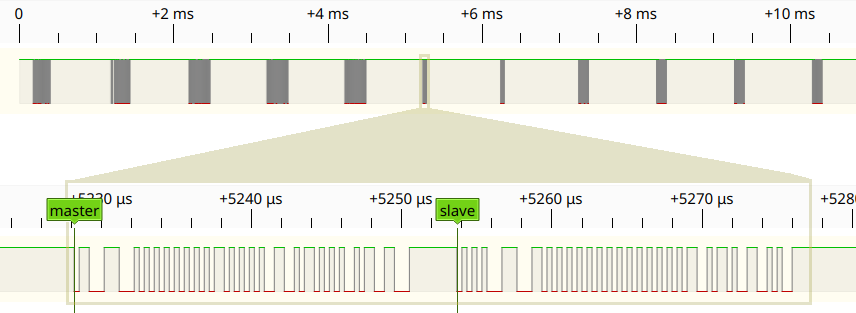
\includegraphics[width=\textwidth]{./Figures/pulseview.png}
    \caption{Visualización de una de las capturas realizadas.}
    \label{fig:pulseview}
\end{figure}

\section{Decodificación de las capturas}
\label{sec:decodificacion}

El siguiente objetivo en la etapa de investigación fue decodificar la información de las tramas capturadas. Para ello se desarrolló un programa en lenguaje Python que toma como entrada una captura en formato binario (un byte por muestra, como se describe en la sección \ref{sec:software}) y produce como salida un reporte de la información decodificada.

El software se compone de dos programas. El primero de ellos, \texttt{mvb\_signal.py}, toma como entrada una captura en formato binario, decodifica los datos codificados en Manchester, y produce como salida un archivo en formato CSV en el que cada línea representa un telegrama y tiene la forma \texttt{<tiempo>,\allowbreak <master>,\allowbreak <slave>}, donde \texttt{<tiempo>} es la marca de tiempo en segundos del telegrama, y \texttt{<master>} y \texttt{<slave>} es el contenido de las tramas en formato hexadecimal, sin incluir los delimitadores y las secuencias de verificación. En el código~\ref{cod:mvbsignal} se muestra un ejemplo de ejecución, en el que se procesa una captura que contiene 4 telegramas.

\begin{lstlisting}[label=cod:mvbsignal,caption=Ejemplo de ejecución de \texttt{mvb\_signal.py}.,float=htbp]
$ python3 mvb_signal.py < captura1.bin
0.0001,4390d6,971e0000008214
0.0011,431bf7,30000f
0.0021,000134,971e07
0.0022,4010c5,04004830580048
\end{lstlisting}

La salida de \texttt{mvb\_signal.py} se puede redireccionar mediante un \textit{pipe} al segundo programa, \texttt{mvbparse.py}, que interpreta la información de las tramas según el protocolo MVB y produce un reporte de la evolución de cada una de las variables identificadas. En el código~\ref{cod:mvbparse} se muestra un ejemplo de ejecución de \texttt{mvbparse.py}.

\begin{lstlisting}[label=cod:mvbparse,caption=Ejemplo de ejecución de \texttt{mvbparse.py}.,float=htbp,basicstyle=\footnotesize\ttfamily]
$ python3 mvb_signal.py < captura2.bin | python3 mvbparse.py
 [[port='0x31b'] [n=   12] [
                  t=  0.001s  0x30000f0c0110000000000000000011a8]],
 [[port='0x353'] [n=    3] [
                  t=  0.212s  0xe2036aa0000000000
                  t=  0.471s  0xe2036ba0000000000
                  t=  0.730s  0xe2036da0000000000]],
\end{lstlisting}

La salida de ejemplo de \texttt{mvbparse.py} indica que se identificaron dos variables, en los puertos \texttt{0x31b} y \texttt{0x353}.
La primera variable fue transmitida en total 12 veces, con un valor de 16 bytes. Se transmitió por primera vez en la marca temporal $0{,}001$ s, con un valor de 16 bytes, y luego se transmitió 11 veces más con el mismo valor.
La variable en el puerto \texttt{0x353} fue transmitida en total 3 veces con un valor de 8 bytes diferente cada vez.

Dado que durante la captura se realizaron diferentes acciones según se mencionó en la sección \ref{sec:capturas} (tomar cabina, abrir y cerrar puertas, etc.), fue posible, analizando la salida producida por el programa, detectar cuáles son las variables que cambian en función del momento en que estas acciones fueron efectuadas. En la figura~\ref{fig:analisis-captura} se muestra, por ejemplo, que la variable en el puerto \texttt{0x1b2} se modifica cada vez que se realizan las acciones de tomar cabina, y seleccionar, abrir y cerrar las puertas.

\begin{figure}[htbp]
	\centering
	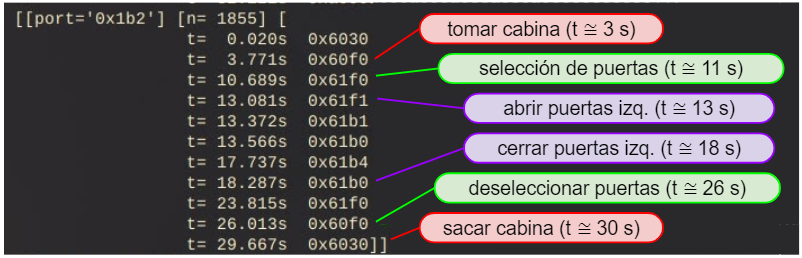
\includegraphics[width=\textwidth]{./Figures/analisis-captura.png}
	\caption[Resultado del análisis de una de las capturas.]{Resultado del análisis de una de las capturas.}
    \label{fig:analisis-captura}
\end{figure}

El software de decodificación está disponible en la plataforma Github \cite{mvbparse-py}. El desarrollo de este prototipo no solo sirvió para proporcionar información valiosa acerca del funcionamiento del bus MVB en las formaciones de Trenes Argentinos, sino también brindó la experiencia necesaria para el posterior desarrollo del software de captura descripto en la sección \ref{sec:software}.

\section{Pruebas del dispositivo de captura}

A continuación se describen los diferentes tipos de pruebas efectuadas para verificar el correcto funcionamiento del dispositivo de captura.

\subsection{Prueba del software de captura}

Para probar el correcto funcionamiento del software de captura (descripto en la sección \ref{sec:software}) se utilizaron las capturas tomadas en la formación ferroviaria (ver sección \ref{sec:capturas}).

Para ejecutar esta prueba se ejecuta el software pasándole como entrada el contenido de una de las capturas en lugar del flujo de datos en tiempo real. Para ello, en una consola se crea un FIFO y se lo alimenta con el contenido de la captura en un ciclo infinito. Se utiliza el comando \texttt{pv} \cite{pv} para limitar el ancho de banda a 12 MB/s:

\begin{lstlisting}
$ mkfifo /tmp/fifo
$ while cat captura.bin; do :; done | pv -L 12M > /tmp/fifo
\end{lstlisting}

En otra consola se ejecuta el software de captura tomando el FIFO como entrada.

\begin{lstlisting}
$ go run cmd/main.go </tmp/fifo
\end{lstlisting}

Esta técnica permite utilizar el software en una PC, como si estuviera conectado al bus MVB.
De esta manera se pudo probar todas sus funcionalidades, tanto en el modo interactivo como en el modo de captura.

\subsection{Prueba de integración de hardware}

% 28 oct 2021?
% 24 nov 2021?

El siguiente paso fue efectuar una prueba de integración del software de captura recibiendo el flujo de datos del VKTECH en tiempo real.
Para ello se utilizó el generador de señal MVB descripto en la sección \ref{sec:generador}, en una configuración como se muestra en la figura~\ref{fig:generador}.
En la figura~\ref{fig:educiaa+vktech} se muestra el banco de medición utilizado en esta prueba.

Esta prueba permitió verificar que es posible utilizar el VKTECH para recibir el flujo de datos en tiempo real.
La prueba se realizó con el software de captura corriendo tanto en una PC como en una Raspberry Pi.

\begin{figure}[htbp]
	\centering
	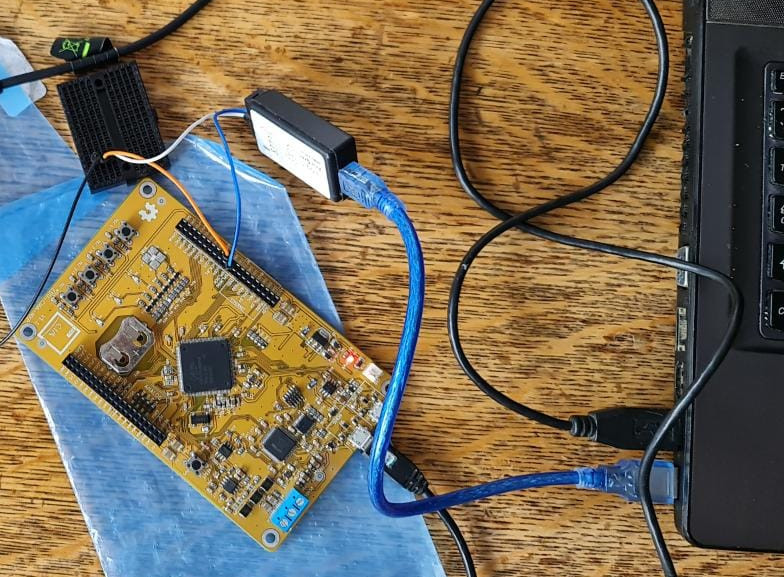
\includegraphics[width=\textwidth]{./Figures/educiaa+vktech.jpg}
	\caption{Banco de medición de la prueba utilizando el generador de señal MVB.}
    \label{fig:educiaa+vktech}
\end{figure}


\subsection{Prueba en una formación ferroviaria}

% 3 dic 2021 (PC)

% 6 ene 2022? (RPI)

La última prueba que se efectuó fue con el dispositivo de captura conectado en el bus MVB en una formación de Trenes Argentinos, como se muestra en la figura~\ref{fig:conexion}.
Se verificó que la conexión del dispositivo de captura no afectó al correcto funcionamiento del resto de los dispositivos conectados en el bus MVB. Cabe destacar que esta prueba se realizó en una formación detenida.

En la figura~\ref{fig:disp-captura-ssh} se muestra una fotografía de la pantalla de la PC utilizada durante la sesión de prueba. En la pantalla se observan dos consolas conectadas a la Raspberry Pi mediante el protocolo SSH. En la consola de la izquierda se ejecuta el comando \texttt{sigrok-cli} para recibir el flujo de datos del VKTECH en tiempo real. En la consola de la derecha se ejecuta el software de captura en modo interactivo.

\begin{figure}[htbp]
	\centering
	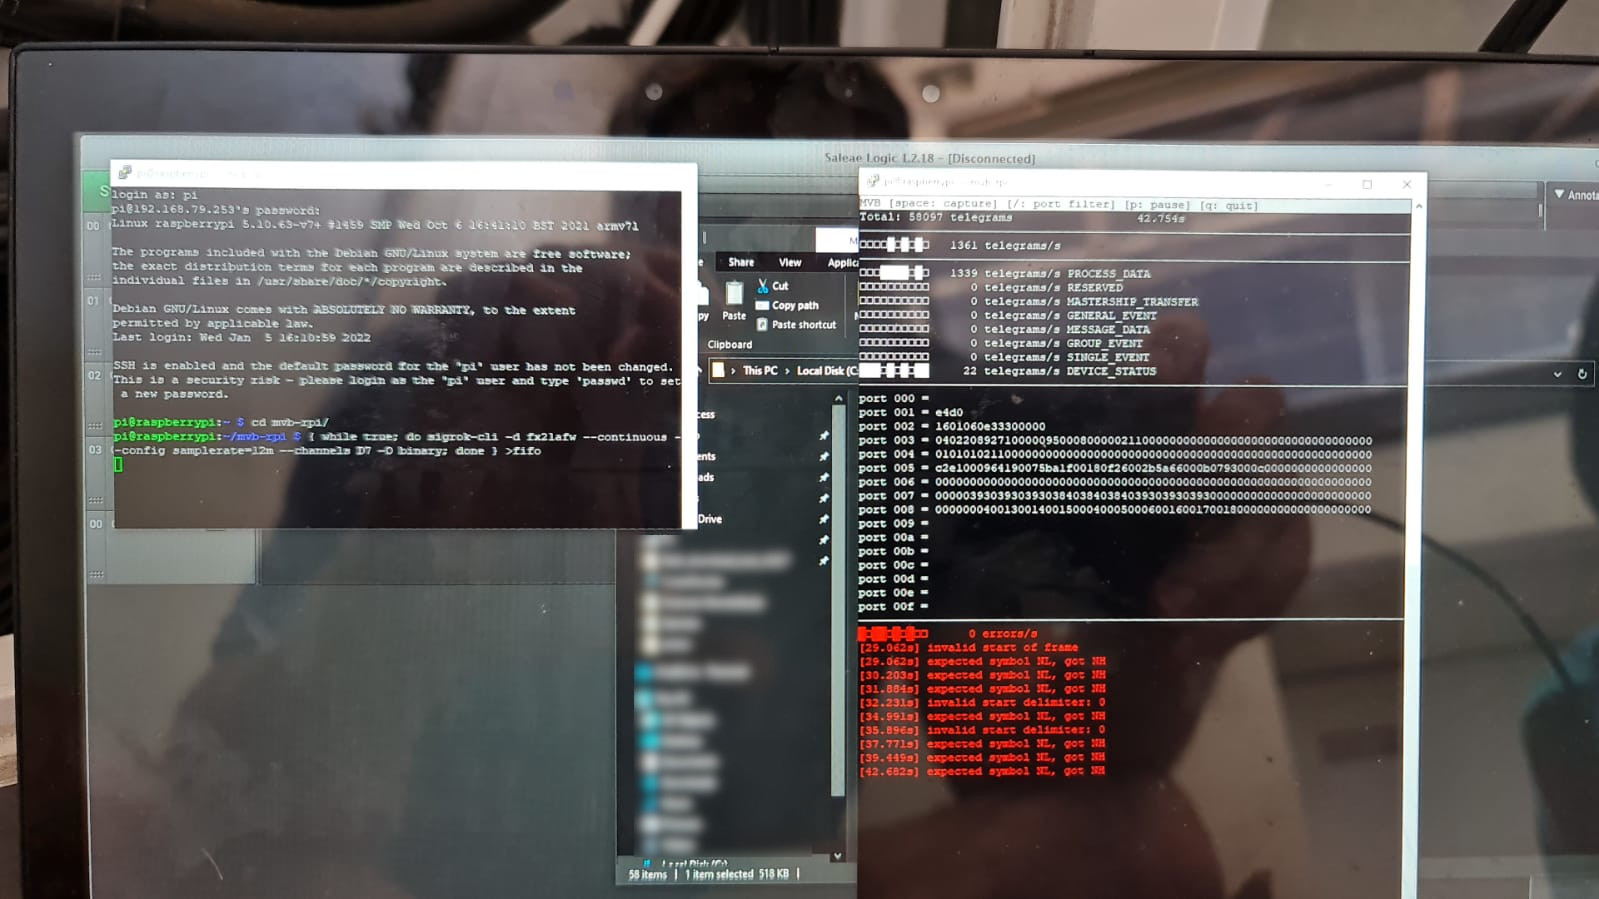
\includegraphics[width=\textwidth]{./Figures/disp-captura-ssh.jpg}
	\caption{Sesión de prueba del dispositivo de captura.}
    \label{fig:disp-captura-ssh}
\end{figure}
 
% Chapter Template

\chapter{Conclusiones} % Main chapter title

\label{Chapter5} % Change X to a consecutive number; for referencing this chapter elsewhere, use \ref{ChapterX}


%----------------------------------------------------------------------------------------

%----------------------------------------------------------------------------------------
%	SECTION 1
%----------------------------------------------------------------------------------------

\section{Conclusiones generales }

La idea de esta sección es resaltar cuáles son los principales aportes del trabajo realizado y cómo se podría continuar. Debe ser especialmente breve y concisa. Es buena idea usar un listado para enumerar los logros obtenidos.

Algunas preguntas que pueden servir para completar este capítulo:

\begin{itemize}
\item ¿Cuál es el grado de cumplimiento de los requerimientos?
\item ¿Cuán fielmente se puedo seguir la planificación original (cronograma incluido)?
\item ¿Se manifestó algunos de los riesgos identificados en la planificación? ¿Fue efectivo el plan de mitigación? ¿Se debió aplicar alguna otra acción no contemplada previamente?
\item Si se debieron hacer modificaciones a lo planificado ¿Cuáles fueron las causas y los efectos?
\item ¿Qué técnicas resultaron útiles para el desarrollo del proyecto y cuáles no tanto?
\end{itemize}


%----------------------------------------------------------------------------------------
%	SECTION 2
%----------------------------------------------------------------------------------------
\section{Próximos pasos}

Acá se indica cómo se podría continuar el trabajo más adelante.
 

%----------------------------------------------------------------------------------------
%	CONTENIDO DE LA MEMORIA  - APÉNDICES
%----------------------------------------------------------------------------------------

\appendix % indicativo para indicarle a LaTeX los siguientes "capítulos" son apéndices

% Incluir los apéndices de la memoria como archivos separadas desde la carpeta Appendices
% Descomentar las líneas a medida que se escriben los apéndices

%% Appendix A

\chapter{Appendix Title Here} % Main appendix title

\label{AppendixA} % For referencing this appendix elsewhere, use \ref{AppendixA}

Write your Appendix content here.
%\include{Appendices/AppendixB}
%\include{Appendices/AppendixC}

%----------------------------------------------------------------------------------------
%	BIBLIOGRAPHY
%----------------------------------------------------------------------------------------

\Urlmuskip=0mu plus 1mu\relax
\raggedright
\printbibliography[heading=bibintoc]

%----------------------------------------------------------------------------------------

\end{document}  
